\section{5. Omics data analysis}

\begin{framed}
\textbf{Learning outcomes}\\
\begin{itemize}
\item 1
\item 2
\item 3
\end{itemize}
\end{framed}

\subsection{Omics data analysis}

\begin{figure}[!htbp]
\centering
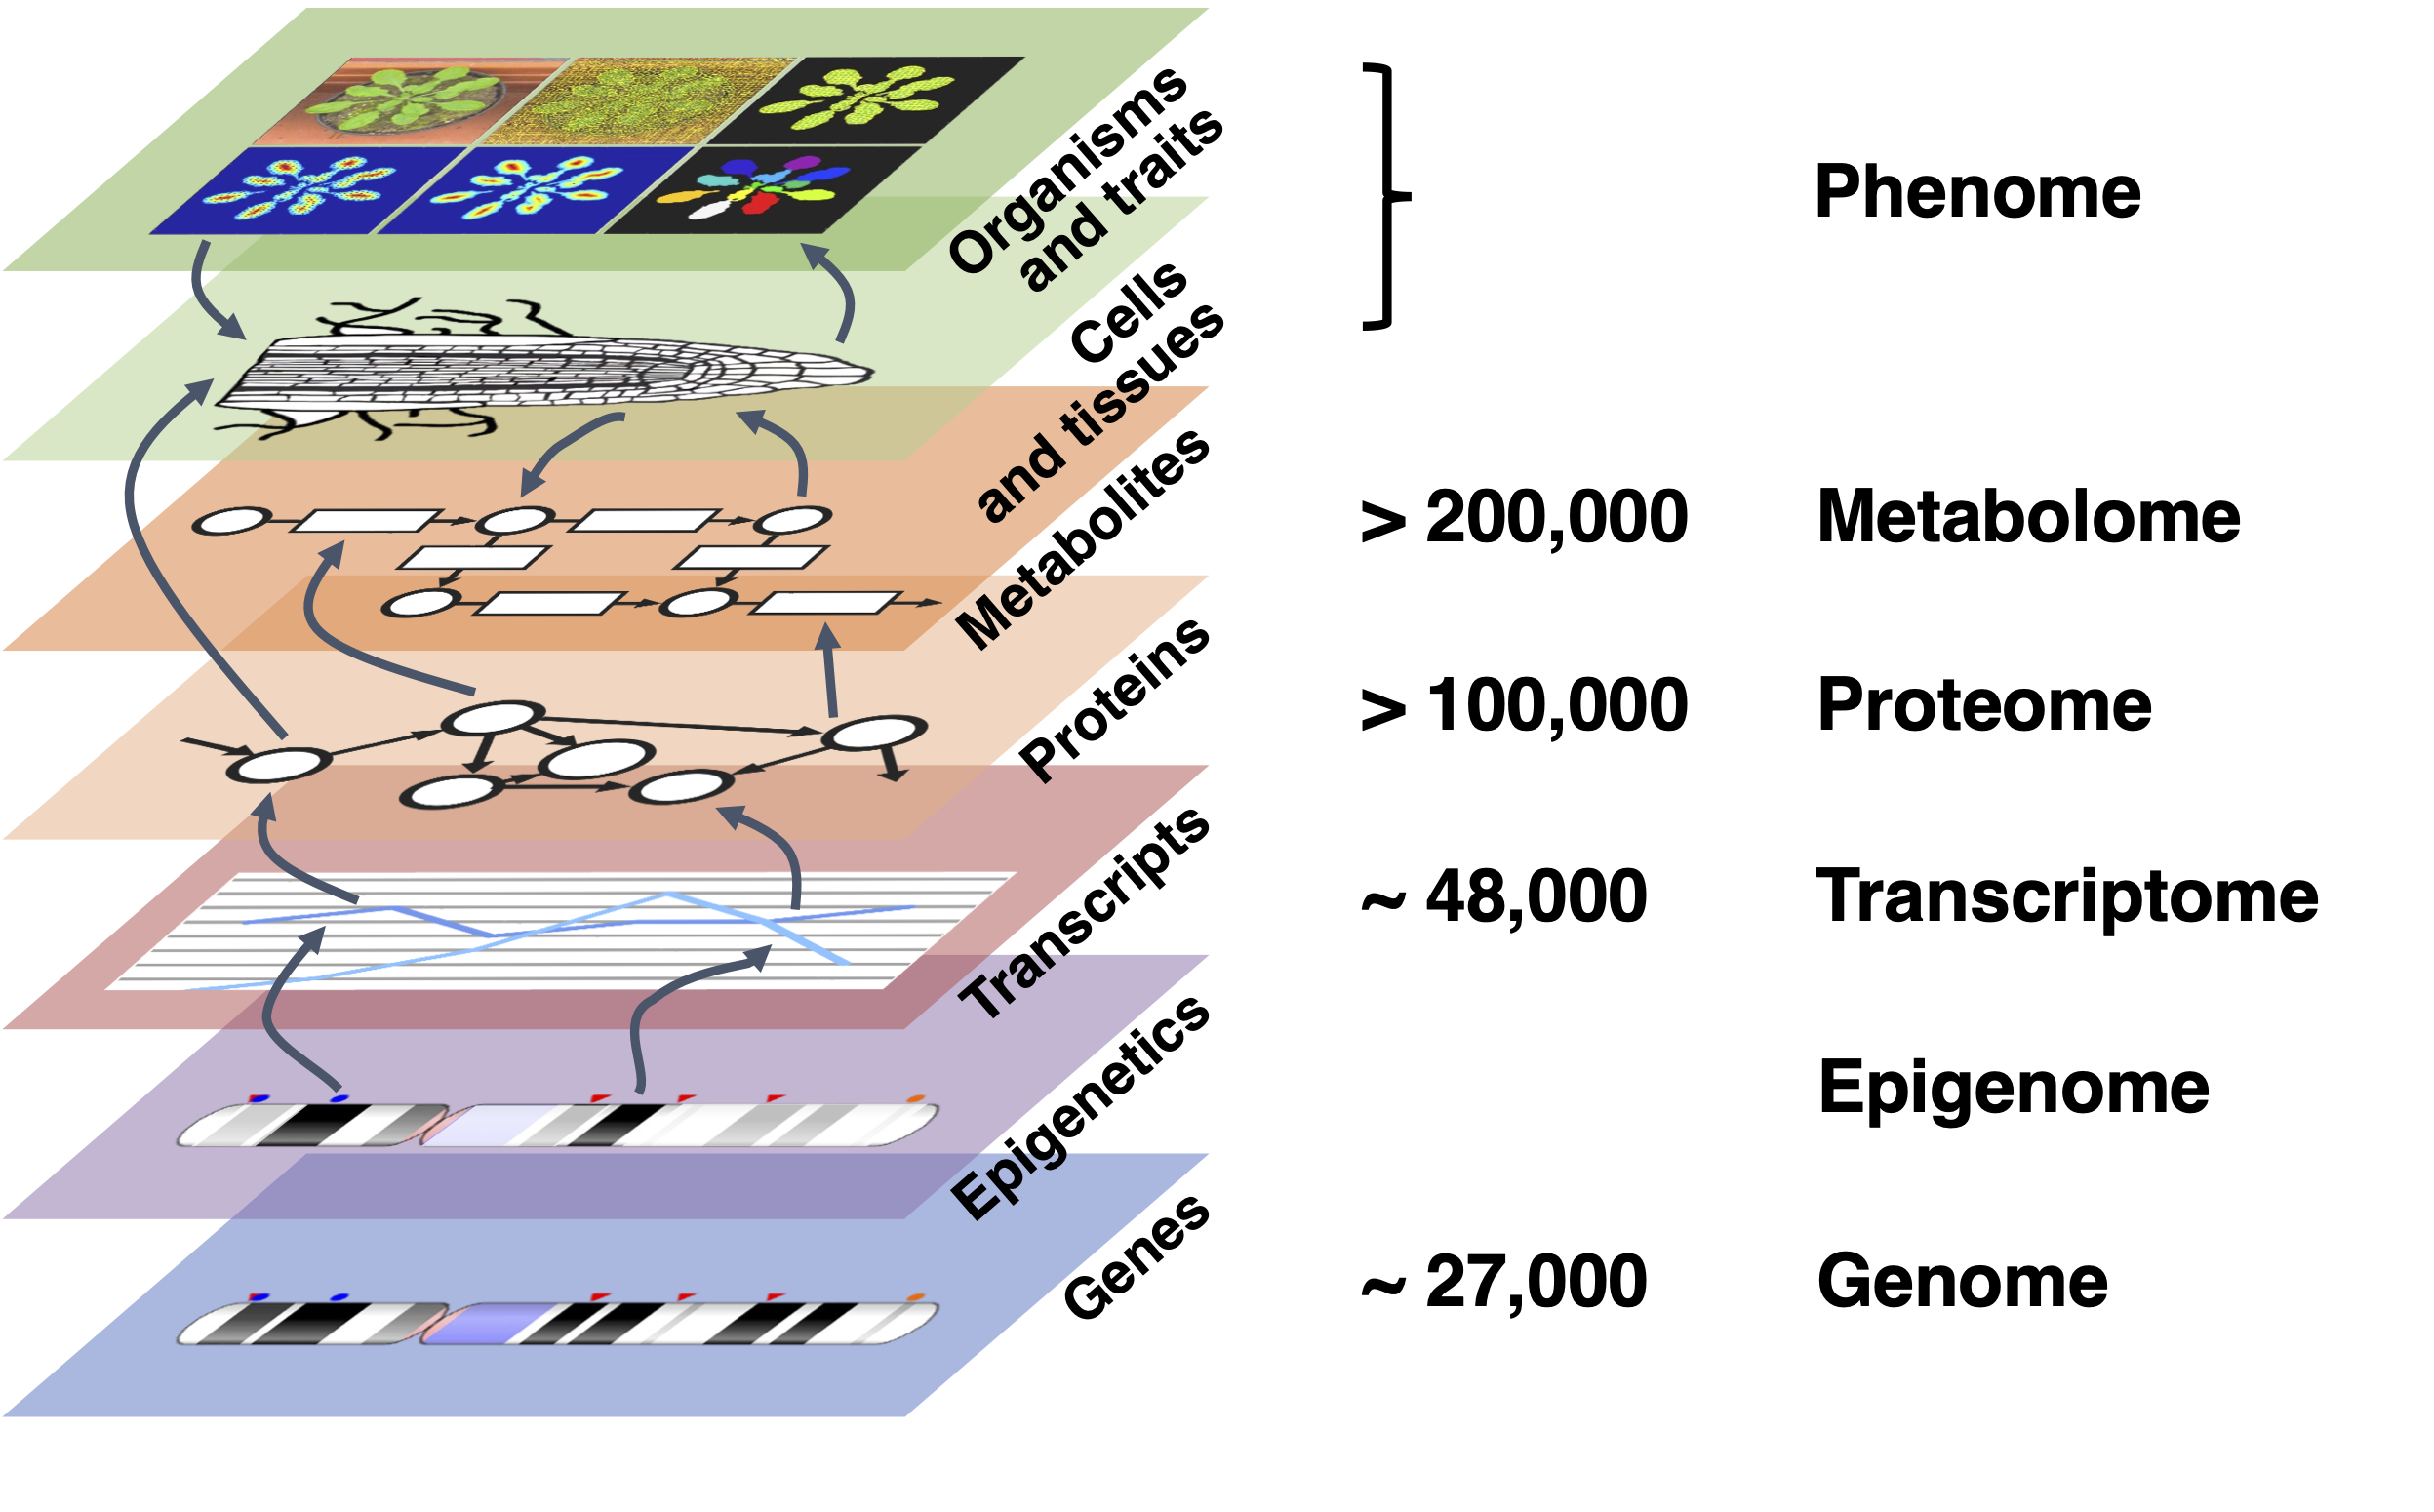
\includegraphics[width=0.7\linewidth]{files/omics-levels-113af087d25808e9162ccac3c0619806.png}
\caption[]{Different -ome levels, here illustrated with numbers for \textit{Arabidopsis thaliana}.
Credits: \href{https://creativecommons.org/licenses/by-nc/4.0/}{CC BY-NC 4.0} \cite{own_5_2024}.}
\label{omics_levels}
\end{figure}


\bigskip
\centerline{\rule{13cm}{0.4pt}}
\bigskip

\begin{quote}
Etymology (from Wikipedia)

\textbf{-ome} (``whole of class'') + \textbf{-ics}, both via international scientific vocabulary and New Latin ultimately from Ancient Greek

Suffix

-omics

(chiefly biology) Forms nouns meaning ``a study of the totality of something''.
\end{quote}

This chapter discusses what we call omics measurements: genomics,
transcriptomics (gene expression), proteomics and metabolomics. Omics
technologies measure the presence, levels and/or interactions of different
types of molecules in the cell, obtaining data for all molecules at once (see Figure~\ref{omics_levels}).
Genomics focuses on the entirety of information that can be derived from
genomes (structure, function, evolution, etc.). Transcriptomics, proteomics,
and metabolomics focus on gene expression, protein, and metabolite levels,
respectively. Finally, phenomics measures the outward appearance and
behavior of cells and organisms.

The concept of genes is central to the dogma of molecular biology; it
therefore makes sense that much early research was invested in sequencing
genomes. These genomes were then annotated for genes, with accompanying
predicted protein sequences. This focus on sequences has dominated much of
the first decades of bioinformatics, leading to the development of the
databases and tools for sequence alignment, phylogeny and sequence-based
prediction of structure that were discussed in earlier chapters. However,
after sequencing the first genomes it became clear that the DNA tells only
part of the entire story: the expression of genes and proteins and their
interactions in processes within and between cells govern how cells and
organisms behave. This led to research in functional genomics and systems
biology, for which computational data analysis of other omics level data
have become indispensable.

Below, genomics will first be introduced, along with the most relevant
technology: sequencing, which is also used for transcriptomics.  This will
be followed by an introduction to functional genomics and systems biology
and brief overviews of transcriptomics, proteomics, metabolomics, and
phenomics, as well as the main types of data analysis involved.


\bigskip
\centerline{\rule{13cm}{0.4pt}}
\bigskip

\subsubsection{Genomics and sequencing}

\begin{figure}[!htbp]
\centering
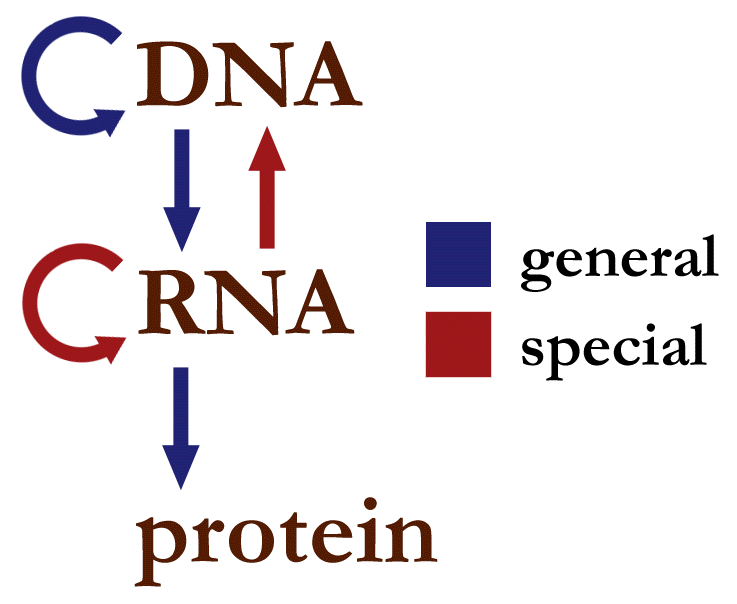
\includegraphics[width=0.45\linewidth]{files/central-dogma-399b6b8c635bffc6272e338818454139.png}
\caption[]{Information flow in the cell. \newline
Credits: \href{https://creativecommons.org/publicdomain/zero/1.0/}{CC0 1.0} \cite{central_dogma_2008}.}
\label{central_dogma}
\end{figure}

DNA is the starting point in the chain of biological information flow. The
central dogma of molecular biology was postulated by Francis Crick in 1958:
cellular processes allow information flow away from DNA to RNA and then to
proteins, not the other way around (Figure~\ref{central_dogma}). From DNA we progress
through transcription and translation towards whole organisms and their
phenotypes. So, it is fitting to start at the beginning. Even before
people knew about DNA and its role as keeper of hereditary information, they
were aware that parental characteristics are inherited by offspring. Around
1866 Gregor Mendel was the first to perform detailed experiments testing
heritability. He first described `units of heredity', later named genes.
Today, we know that genes are encoded in the DNA in our cells. Our
understanding of genes has expanded to a more complex concept, focused on
stretches of DNA coding for proteins or RNA. The term genome was originally
used to describe all genes in an organism or cell, but now refers to the
full DNA content of a cell.

\begin{framed}
\textbf{Box 5.1: The history of DNA sequencing and the Human Genome Project}\\
The history of genome sequencing is closely linked with the Human Genome
Project (HGP) and the HGP was the major driver in technology development.
Everything started in 1977 with the first DNA sequencing method developed
by Sanger, Maxam, and Gilbert, and this allowed the first genome to be
sequenced: Phi X bacteriophage.
Another important mile stone was the development of PCR (Polymerase Chain Reaction)
in 1985, which enabled DNA amplification. The first automated sequencer (AB370A)
appeared in 1986.

With continued technological developments, new genome sequences started appearing
slowly at first. The Epstein-Barr virus was sequenced in 1983. The first
bacterial genome, \textit{Haemophilus influenzae}, was sequenced in 1995, followed by the first
archaeal genome sequence of \textit{Methanococcus jannaschii} in 1996. In the same
year followed the first eukaryotic genome, that of \textit{Saccharomyces
cerevisiae} (baker's yeast). \textit{Escherichia coli}, the main bacterial model
organism, was sequenced in 1997.

The human genome project formally started in 1988, although sequencing did not start
until around 1990. The human genome was completely sequenced with Sanger sequencing
technology (which is described below) and a first draft genome, covering 90\%
of the estimated 3.2 billion base pairs, was published in Nature in 2001,
with a final genome in 2003 (Figure~\ref{landmarks_in_genetics}).
One of the most surprising findings was that the human genome only contained roughly 20,000 genes, far less than the
estimated 50,000-140,000. The entire project is estimated to have cost \href{https://www.genome.gov/about-genomics/educational-resources/fact-sheets/human-genome-project}{\$3
billion}.
In 2021 the first true telomere-to-telomere assembly of the human genome was
assembled using the third generation technologies described below: PacBio,
Oxford~Nanopore and Hi-C.

\begin{figure}[!htbp]
\centering
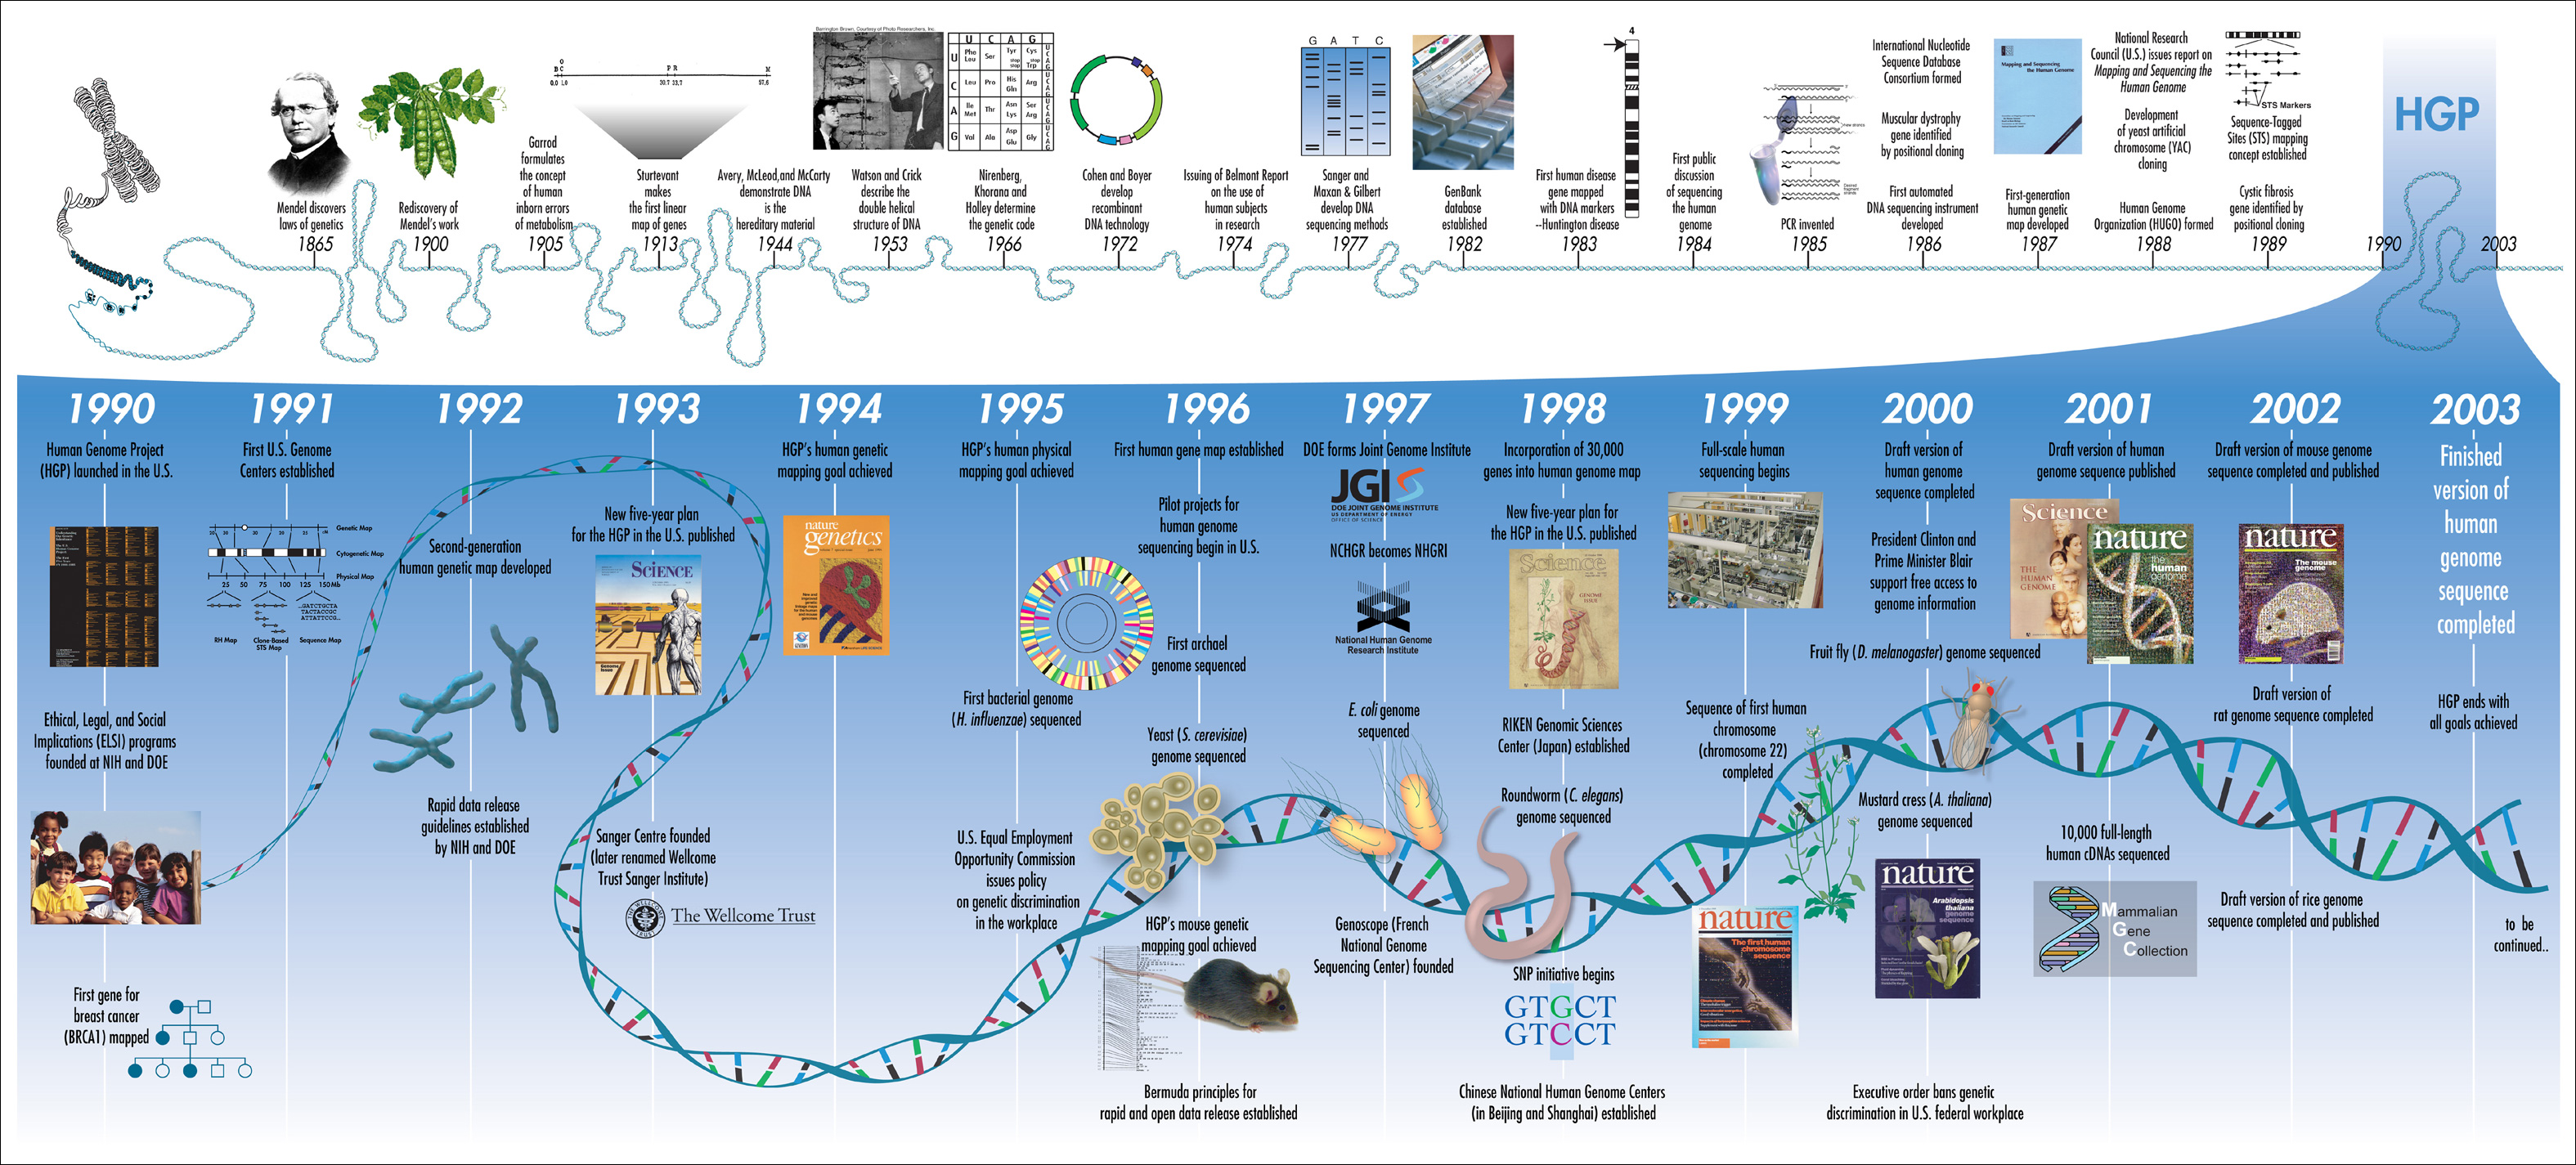
\includegraphics[width=0.7\linewidth]{files/Fig_Box1_Human_Genom-3c06ee6d5a13d224243c3d6e3f1f871c.jpg}
\caption[]{Timeline of the Human Genome Project \newline
Credits: \href{https://creativecommons.org/licenses/by/2.0}{CC-BY 2.0} \cite{timeline_HGP_2003}.}
\label{landmarks_in_genetics}
\end{figure}
\end{framed}

% #% In the last line of box 5.1 it describes third generation technologies, amongst which Hi-C. However, the section [chapter5_3rd_generation] lacks information on Hi-C.


\bigskip
\centerline{\rule{13cm}{0.4pt}}
\bigskip

\paragraph{Genomes}

The history of genome sequencing and the importance of the human genome project
in the development of sequencing methods is described in Box~1.
With the rapid evolution of sequencing technology, our understanding of
genomes and their content has grown as well. We now know that genomes vary
greatly in terms of size, chromosome numbers, and ploidy (Figure~\ref{gene_ploidy}),
as well as gene content (Table~\ref{w5t1}). Genome sizes range from 100kb in
bacteria to more than 100Gb (Giga basepairs) in plants. Humans have a genome size of 3.2Gb.

\begin{table}
\centering
\caption[]{Genome size and number of genes of model species}
\label{w5t1}
\begin{tabular}{p{\dimexpr 0.200\linewidth-2\tabcolsep}p{\dimexpr 0.200\linewidth-2\tabcolsep}p{\dimexpr 0.200\linewidth-2\tabcolsep}p{\dimexpr 0.200\linewidth-2\tabcolsep}p{\dimexpr 0.200\linewidth-2\tabcolsep}}
\toprule
Species & Genome size & Number of genes & Number of transcript & Average gene density (kb) \\
\hline
\textit{E. coli} & 4.6 & 4288 & 4688 & 1.1 \\
\textit{S. cerevisiae} & 12.1 & 6600 & 7127 & 1.8 \\
\textit{C. elegans} & 100 & 19985 & 60000 & 5 \\
\textit{D. melanogaster} & 143.7 & 13986 & 41620 & 10.2 \\
\textit{A. taliana} & 119.1 & 27562 & 54013 & 4.3 \\
\textit{H. sapiens} & 3100 & 20077 & 58360 & 154.4 \\
\bottomrule
\end{tabular}
\end{table}

Not only the genome size varies greatly, in eukaryotes the number of chromosomes and chromosomal copies
(ploidy) do too. Chromosome numbers range from 4 in fruit fly (\textit{Drosophila})
to 23 in human to 50 in goldfish and 100+ in some ferns.~Similarly, ploidy
ranges from haploid (single set of chromosome(s), ploidy of N) and diploid
(two copies, ploidy of 2N) to polyploid (more than 3 copies), with at the
extreme end ferns with ploidy levels of over 100. Gene numbers also vary
per species; at the low end, bacterial endosymbionts have 120+ genes,
whereas most higher eukaryotes (including humans) have between 15,000 and
25,000 genes and some plants can have more than 40,000 genes -- rice has over
46,000.

\begin{figure}[!htbp]
\centering
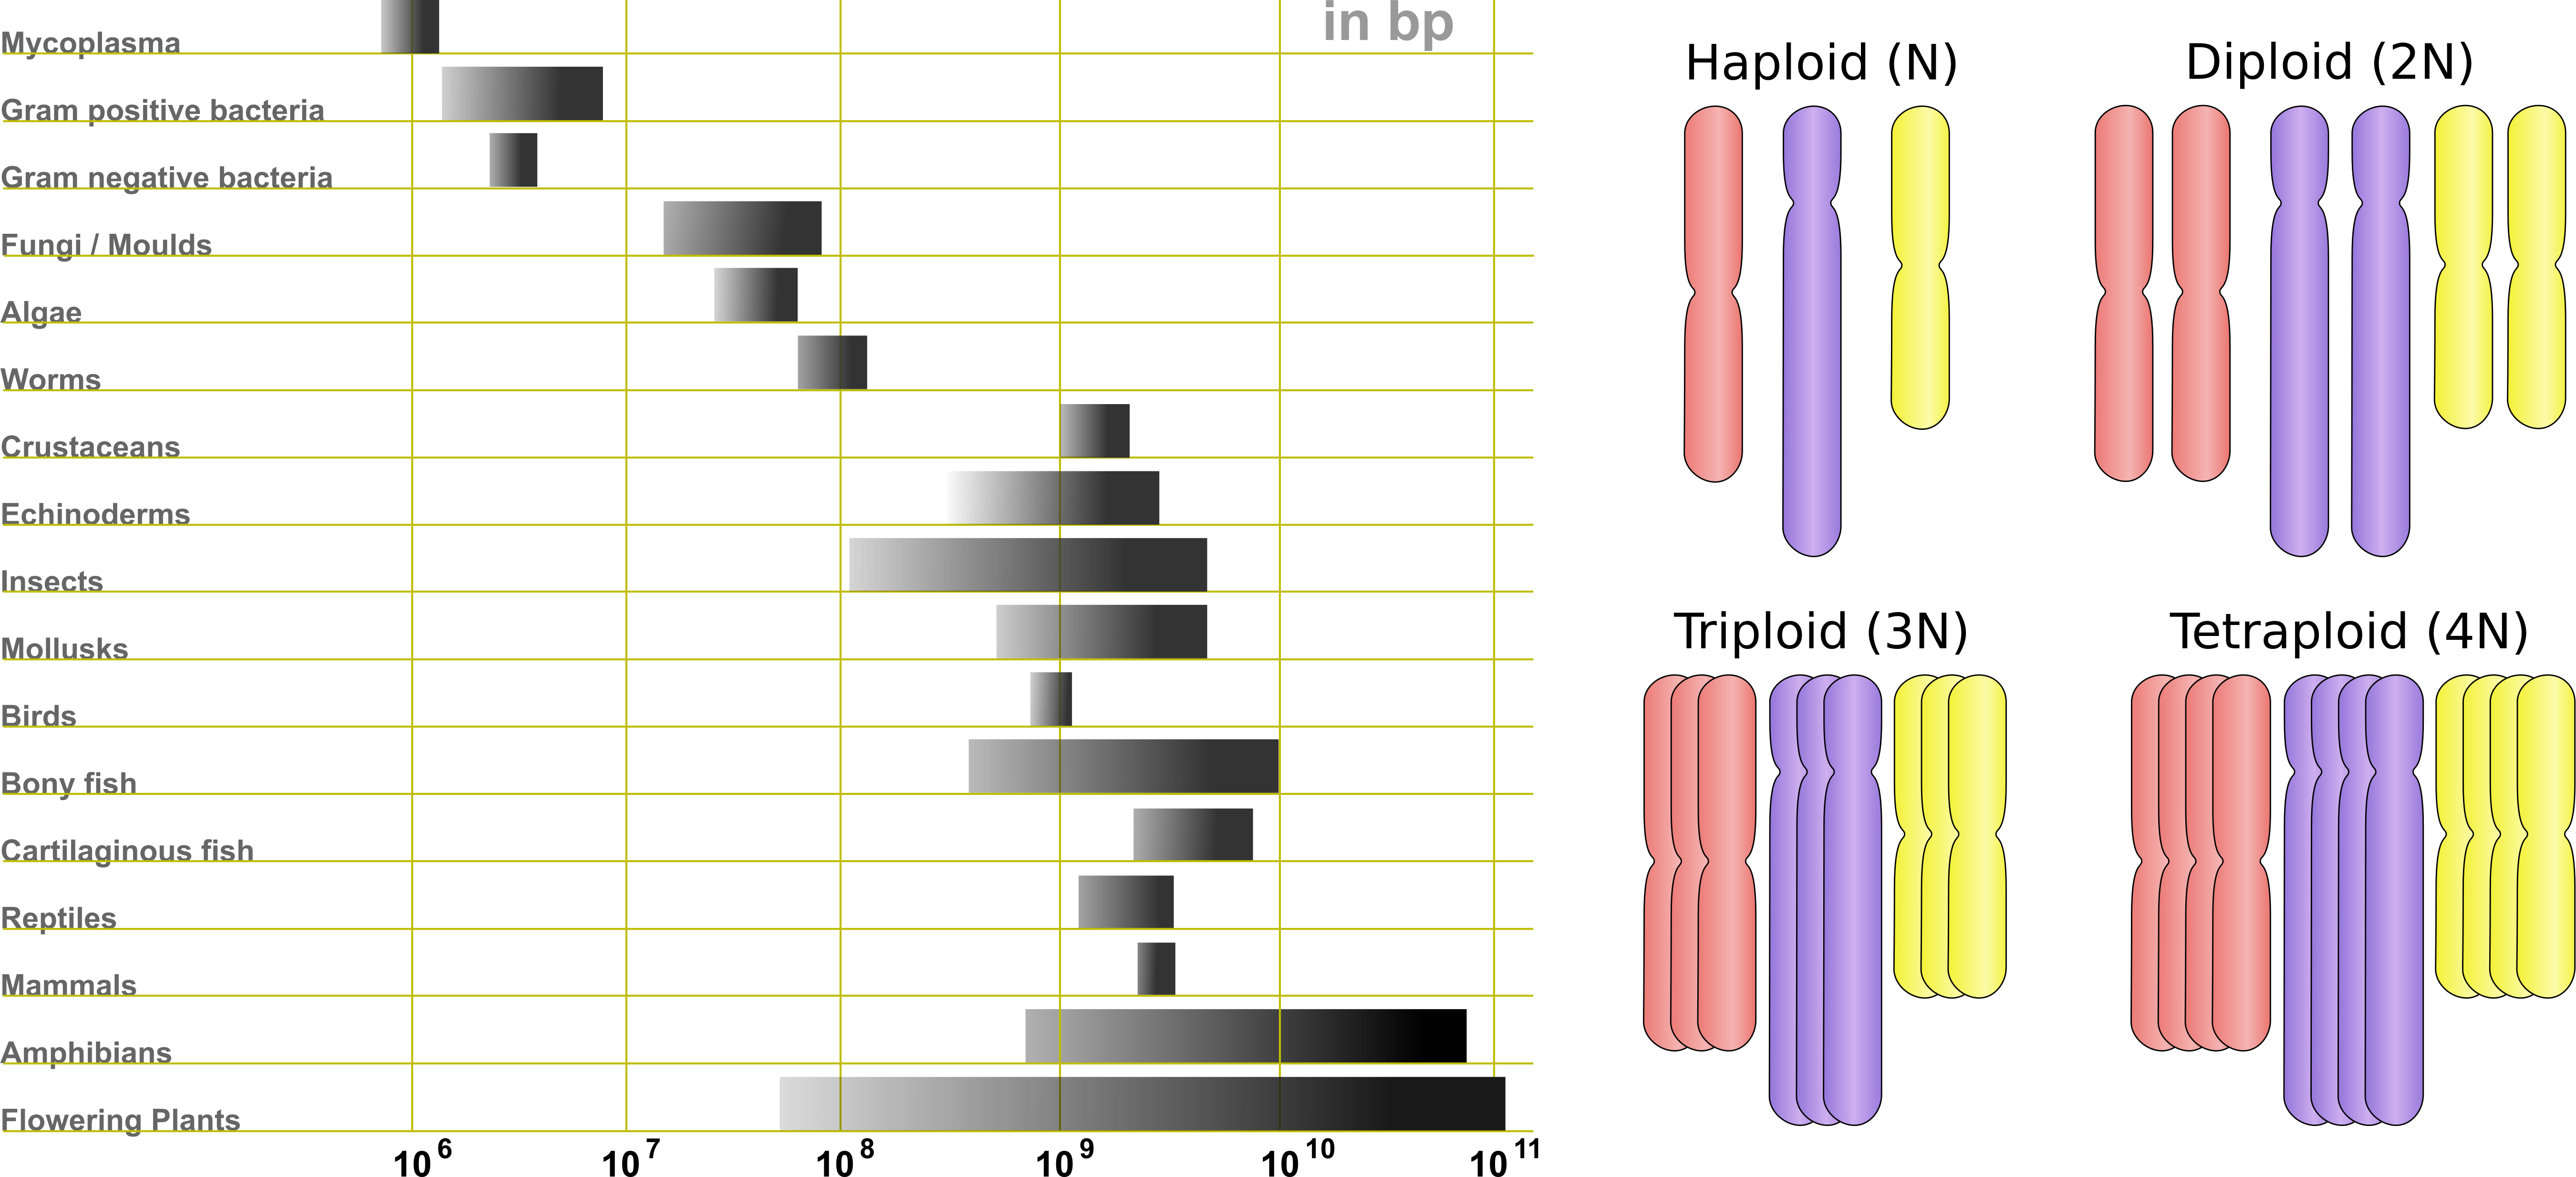
\includegraphics[width=0.7\linewidth]{files/gene-ploidy-570084bb3b9a1da9cf458ffc6db69b85.png}
\caption[]{Left, variety of genome sizes. Credits: \href{https://creativecommons.org/licenses/by-sa/3.0/}{CC BY-SA 3.0} \cite{gene_ploidy_2010};
right, examples of ploidy. Credits: \href{https://creativecommons.org/licenses/by-sa/3.0/}{CC BY-SA 3.0} \cite{gene_ploidy_2011}.}
\label{gene_ploidy}
\end{figure}

\begin{framed}
\textbf{Box 5.2: Size does(n't) matter?}\\
Genomes come in all shapes and sizes. The smallest known (non-viral) genome
is that of the bacterial endosymbiont \textit{Nasuia deltocephalinicola}, which
only consists of 112,091 nucleotides encoding 137 proteins. The largest
genomes known to date are marbled lungfish and the plant \textit{Fritillaria
assyriaca} with 130,000,000,000 nucleotides (130Gb), although the amoeboid
\textit{Polychaos dubium} is purported to have a genome size of 670Gb. Genome size
is not necessarily correlated with the number of genes in the genome (see
also Table~\ref{w5t1}). Number of protein coding genes in turn is not
correlated entirely with organism complexity.
\end{framed}


\bigskip
\centerline{\rule{13cm}{0.4pt}}
\bigskip

\subparagraph{Genome sequencing technologies}

The process of generating a genome starts with DNA sequencing, the detection
of nucleotides and their order along a strand of DNA. Conceptually, there
are three ways of sequencing:

\begin{itemize}
\item Chemical sequencing relies on step-by-step cleaving off the last nucleotide from a chain and identifying it.
Mainly due to the use of radioactive labels, this method was never widely used.


\item Sequencing-by-synthesis involves synthesizing a complementary strand base by base and detecting insertion at each position.
This is currently the most widely used method, and various implementations are available.
It is also referred to as Next-Generation~Sequencing (NGS).


\item Direct sequencing involves directly measuring the order of nucleotides in a strand of DNA, which has only recently become feasible and is thus far only implemented in Oxford~Nanopore~sequencing.
\end{itemize}

Different technologies vary wildly in the length of DNA sequences they produce
(the read length) and their throughput, which together determine the
coverage: the (average) number of times each base in the genome is represented in a read.
For some purposes, such as genome assembly, it is essential that the
coverage is sufficiently high - depending on read length, between 50x to
100x. A number of sequencing devices and their
capabilities in terms of read length and yield per run are shown in
Figure~\ref{sequencing_technology}.

Sequencing technologies also vary in the accuracy of base-calls. This accuracy is measured using quality
or Q scores and they represent the probability that a base-call is incorrect. A higher Q-score is better.
The most commonly used cut-off value is Q30 which corresponds with an incorrect base-call probability
of 1 in 1000 and therefore an accuracy of 99.9\%.

\begin{figure}[!htbp]
\centering
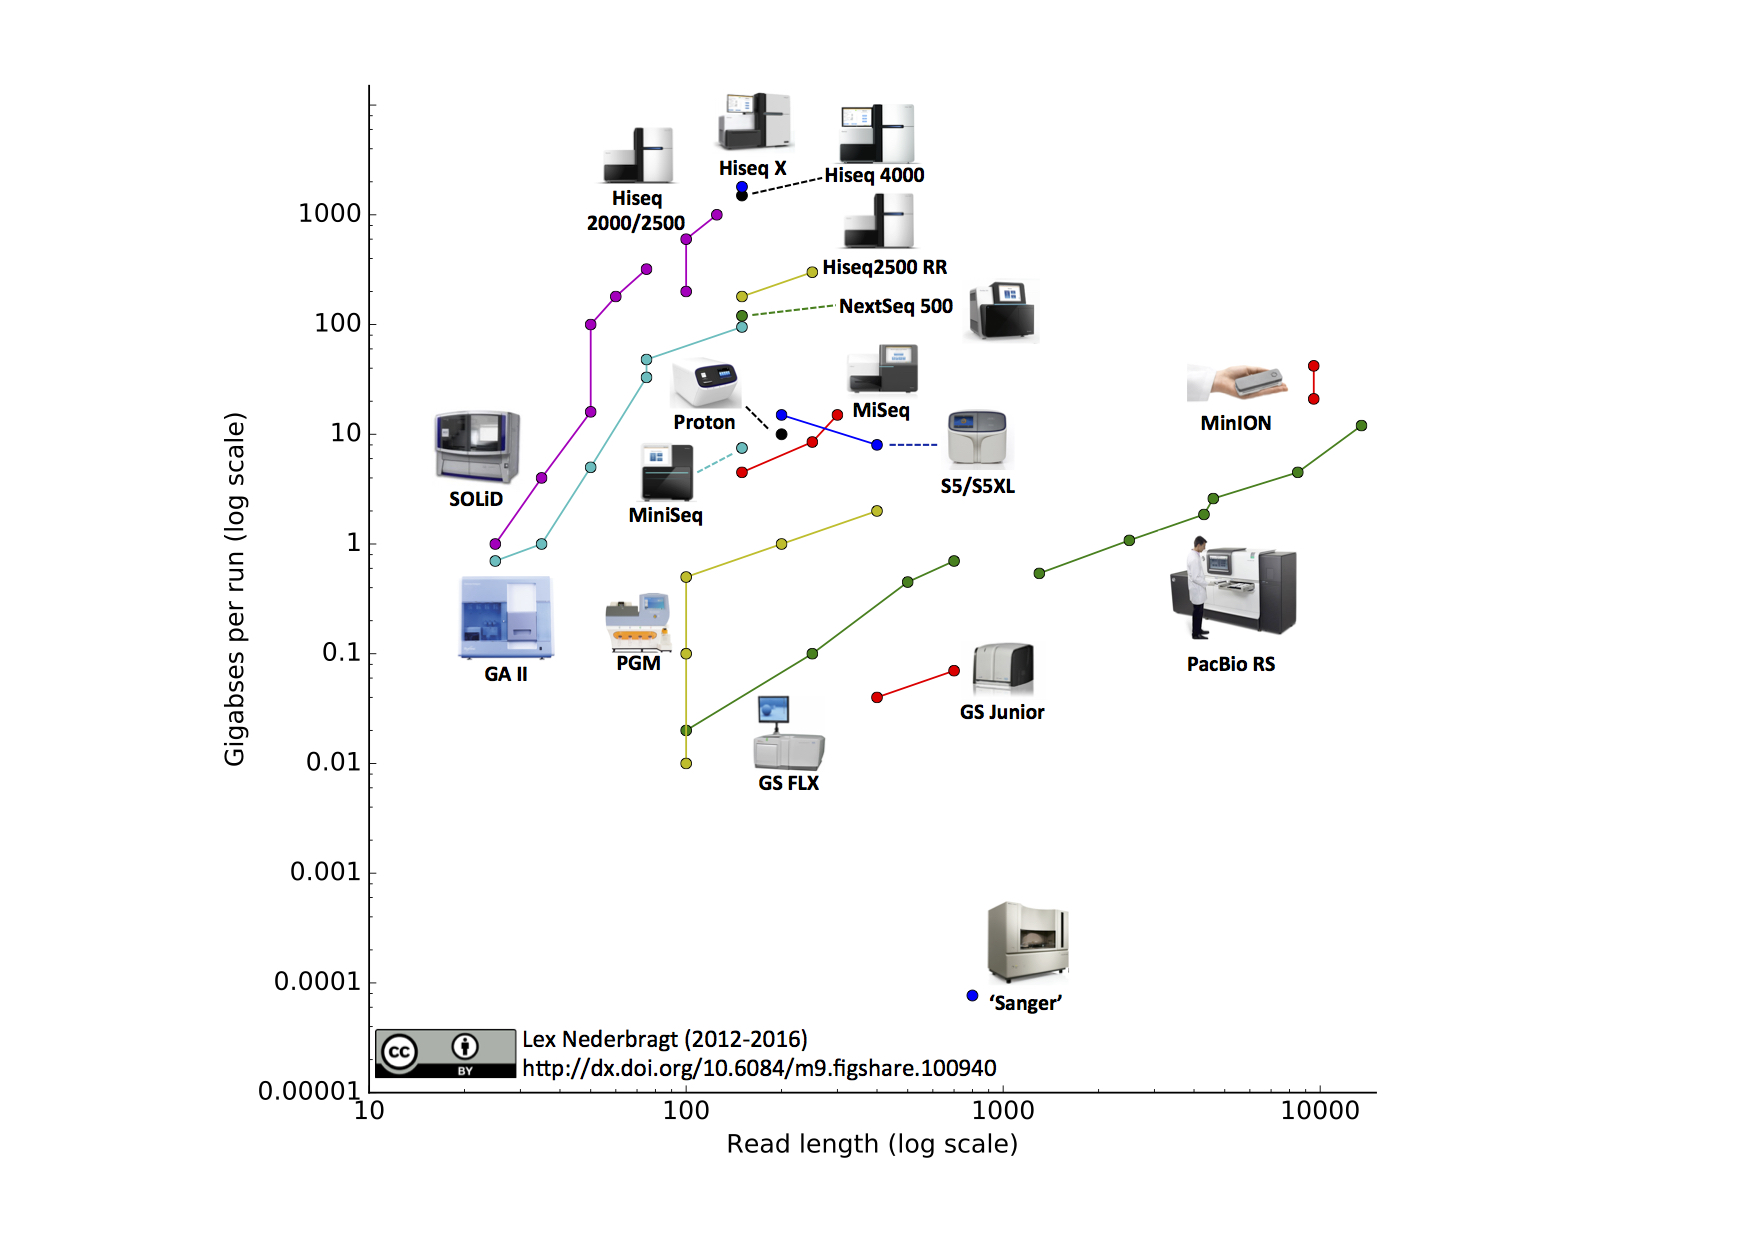
\includegraphics[width=0.7\linewidth]{files/sequencing-technolog-6f4ab9c7a9ccd54746b2b62c8739cea6.jpg}
\caption[]{Sequencing technology, with yield per run vs. read length. Note the
logarithmic scales. Multiple dots per technology indicate improvements in
read length and/or yield due to upgrades. This figure is already outdated
with higher yields produced by the Illumina NovaSeq and longer reads by both
Oxford Nanopore MinION/PromethION and Pacbio Sequel II devices. Credits:
\href{https://creativecommons.org/licenses/by/4.0/}{CC BY 4.0} \cite{sequencing_technology_2016}.}
\label{sequencing_technology}
\end{figure}


\bigskip
\centerline{\rule{13cm}{0.4pt}}
\bigskip

\subparagraph{Sanger sequencing}\label{chapter5_sangersequencing}

Sanger sequencing was the first `high-throughput' method of DNA sequencing.
For more details on its history and how it works, see Box~3.

\begin{framed}
\textbf{Box 5.3: Sanger sequencing}\\
Developed in 1977 by Fred Sanger and colleagues, the protocol was first
largely manual until it was automated in 1985 by Applied Biosystems. Sanger
sequencing uses the chain-termination method (Figure~\ref{sanger}).

\begin{figure}[!htbp]
\centering
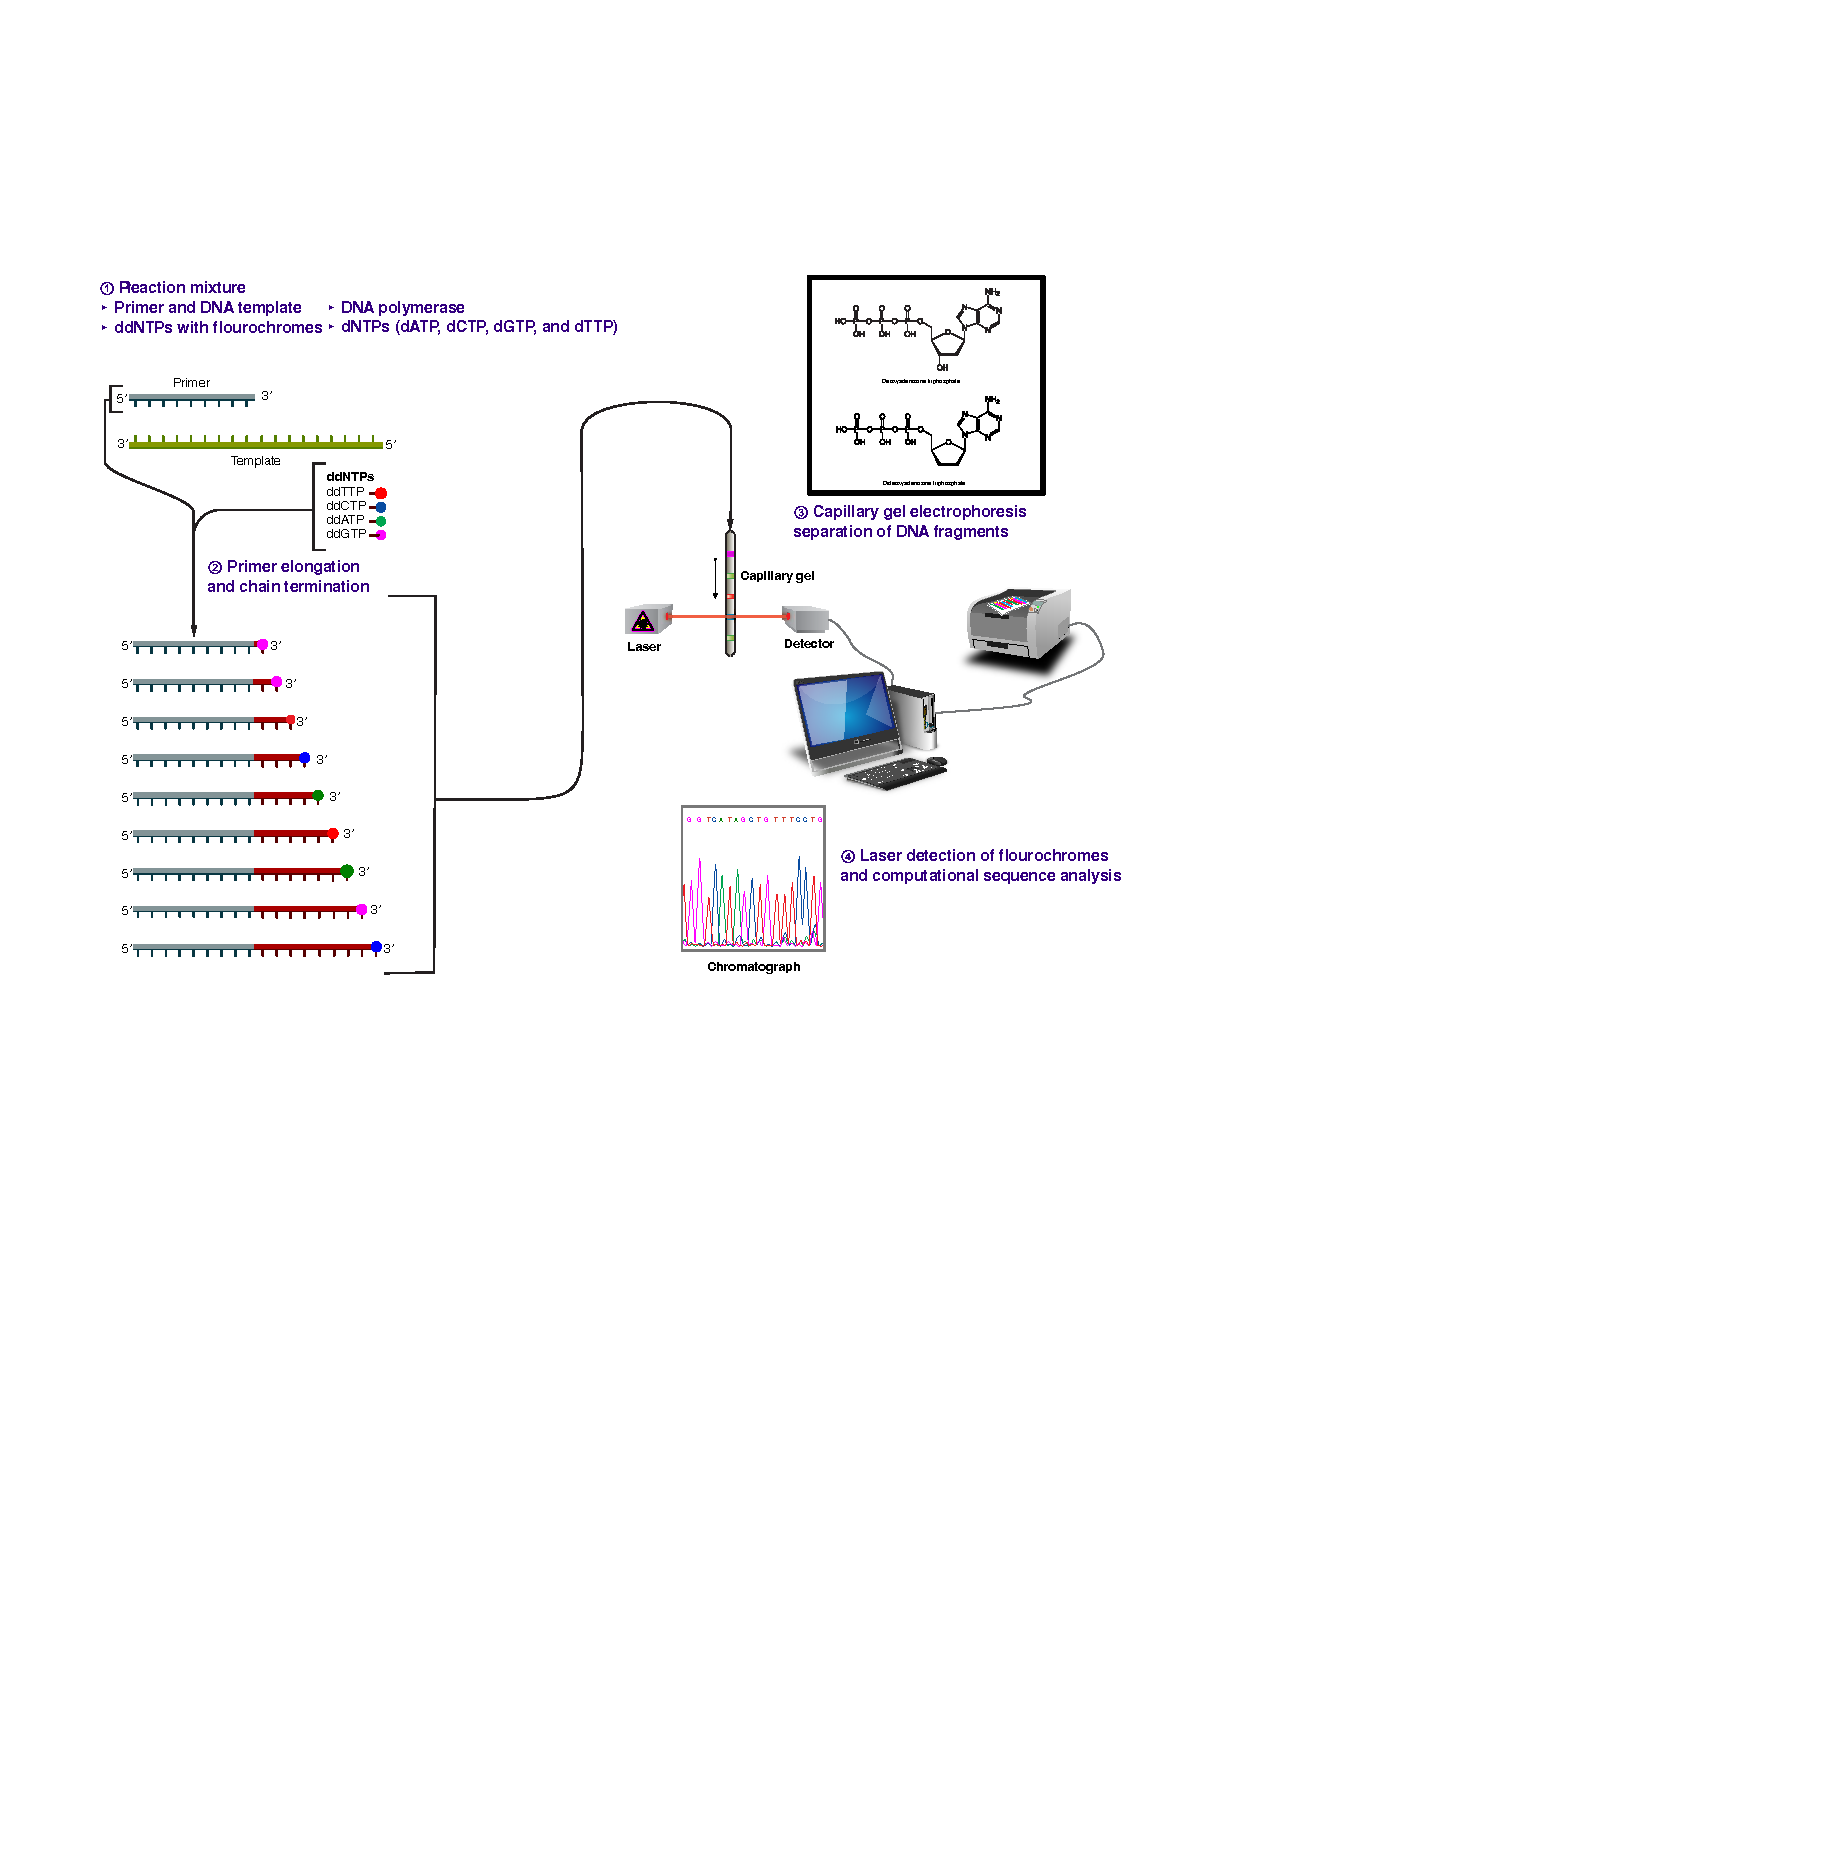
\includegraphics[width=0.7\linewidth]{files/sanger-8b9e6bd1f6eb7c5c40373699fe4a893d.pdf}
\caption[]{Chain termination (Sanger) sequencing.
Credits: \href{https://creativecommons.org/licenses/by-sa/3.0/}{CC BY-SA 3.0} \cite{sanger_2012}.}
\label{sanger}
\end{figure}

In a first step, genomic DNA is purified and sheared into fragments of the desired length. For Sanger
sequencing the fragment length is around 1,000 nucleotides. Shearing is
done either mechanically or chemically, and resulting fragments are not all
exactly equally long: they are distributed around the target fragment size.

\begin{figure}[!htbp]
\centering
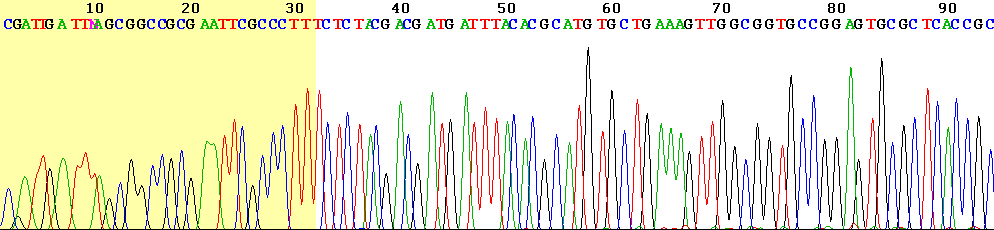
\includegraphics[width=0.7\linewidth]{files/sanger-signal-d3e41d780e1b2a30990d840a13be80b4.png}
\caption[]{Sanger sequencing signal, with low quality bases at the start of the read.
Credits: \href{https://creativecommons.org/publicdomain/zero/1.0/}{CC0 1.0} \cite{sanger_signal_2005}.}
\label{sanger_signal}
\end{figure}

Template DNA fragments are amplified in a PCR reaction using a primer and
DNA polymerase. Each sample is amplified in 4 separate reactions, one for
each nucleotide (A, T, C, G). In each of these reactions, a small
DNA polymerase. In each of these reactions, a small
proportion of modified nucleotides (ddNTP) is added to the normal
nucleotides (dNTP). These modified nucleotides are designed to stop the
elongation of the strand and are linked to a label by which they can be
identified. This leads to a collection of partially amplified fragments of
template DNA. The length of each fragment was originally measured by the
identified. distance the fragment travelled on a gel, in later setups by the time it
took to pass through a capillary.  The label on the last nucleotide then
identifies the base at a given position and a peak pattern is generated.
From a signal of peak patterns (Figure~\ref{sanger_signal}), the sequence can be read
off automatically. Sanger sequencing produces read lengths between
700-1,000 nucleotides; after this, the quality of the base calling drops too
far to be useful. The quality at the beginning of a read is generally too
low to be used (Figure~\ref{sanger_signal}). Another problem with Sanger sequencing is
the detection of homopolymers (the same nucleotide occurring multiple
times), as the peak height of the signal decreases the longer the stretch
is. This makes it difficult to differentiate between 3, 4 and 5 nucleotides
of the same base. Sanger sequencing machines can sequence 96 fragments in
parallel, making it comparatively low throughput.
\end{framed}

Sanger sequencing needs many copies of a single DNA fragment to be present in
the sequencing reaction. This meant that in the sample preparation step
fragments were cloned using either PCR or other large scale amplification methods.
The requirement of uniqueness is the biggest drawback of Sanger sequencing.

\begin{framed}
\textbf{Important to know about Sanger sequencing}\\
\begin{itemize}
\item it is the original sequencing platform
\item was used to sequence the first human genome
\item it produces reads of up to 1000bp long with a quality of 99.9\% (Q30)
\item it is a low throughput method
\item it can only sequence on fragment at a time.
\end{itemize}
\end{framed}

Sanger sequencing was the main sequencing platform until around 2007. From
2004 onwards, it was increasingly superseded by the what we call
next-generation sequencing (NGS) methods. Today it is still used, among
others to sequence PCR products to validate variants, to determine the
orientation of genes in cloned vectors, or in microsatellite studies.


\bigskip
\centerline{\rule{13cm}{0.4pt}}
\bigskip

\subparagraph{Next generation sequencing}\label{chapter5_ngs}

Next-generation sequencing (NGS) technologies allow much higher throughput
at far lower cost than Sanger sequencing, although it comes at a price:
shorter reads and lower base-calling accuracy. These newer devices now
produce billions of reads per sequencing run. Describing all of these
methods in detail is beyond the scope of this course.

As with Sanger sequencing, NGS methods rely on amplification of a library of
input DNA fragments to enhance the signal of the actual sequencing step.
Most sequence data is nowadays generated by Illumina technology (or 3rd
generation methods, see the next section) which allows for massive parallel
sequencing of reads. How Sequencing-by-synthesis and Illumina patterned flow
cells work is explained in Box~4.

\begin{framed}
\textbf{Box 5.4: Illumina sequencing}\\
Illumina sequencing uses
bridge-amplification, where the PCR reaction takes place directly on a
flow-cell surface. In the library preparation step, a
forward and reverse adapter are ligated to the ends of a single strand
template fragment. The complementary sequences for the adapters are ligated
to a flow-cell as PCR primers. The initial template sequence (with
adapters) will then form a double stranded bond with one of the primers on
the flow-cell surface. The fragment is next copied in a
standard PCR reaction, but with the end firmly attached to the surface. The
DNA is denatured to go from double stranded to single stranded again and the
original template is washed away, leaving a single fixed copy. The end of
that strand can then form a bridge with a neighbouring empty primer of the
other end and the reaction is repeated, ending in first two fixed fragments
and subsequently thousands of identical fragments near each other. In the
sequencing step, a final PCR then uses fluorescent dye
terminated NTPs, which are washed across the surface in each cycle. A
camera detects the colour, the dye is cleaved off and the steps are repeated
for the length of the sequencing reaction:

Current models us a so-called patterned flow-cell, were the template fragments
fall into a tiny well and the amplification step takes place in the wells:
\end{framed}

\begin{framed}
\textbf{Important to know about Illumina sequencing}\\
\begin{itemize}
\item all reads in one run have the same length, defined by the number of cycles (20-350bp).
\item due to the fixed read length it is possible that the sequenced reads contain
primer sequences (if the DNA fragment was shorter than the number of
cycles); these always need to be removed
\item reads can be sequenced from one primer end only, which yields
so-called single end reads, or from both primer ends, which gives paired end
reads, i.e. two reads that originate from the same molecule with a distance
that is approximately known
\item reads have a base accuracy of about 99.99\% (Q40)
\item it is very high throughput: The number reads obtained in a
single run range from millions to billions, depending on the model
\item fragments with extreme GC content are less likely to be sequenced, which can
lead to incomplete genome assemblies or coverage
\item is good for variant detection (see Variants)
\end{itemize}
\end{framed}

Overall, Illumina reads are cheap, short and highly accurate.


\bigskip
\centerline{\rule{13cm}{0.4pt}}
\bigskip

\subparagraph{3rd Generation sequencing}\label{chapter5_3rd_generation}

After the success of NGS, alternative so-called 3rd generation technologies
were introduced to overcome some of the shortcomings, mainly the limited
read length. All produce longer reads at lower yields, and generally have a
slightly higher error rate than the methods described previously. They also perform
what is called real-time sequencing: Each DNA fragment is sequenced completely in a
continuous way, there is no need for individual cycles like in NGS.

\subparagraph{PacBio}\label{chapter5_pacbio}

The most established method is PacBio single molecule real time (SMRT)
sequencing. Compared to other methods it does not include a PCR step to
amplify the signal of the template DNA. Instead, during the sequencing of
an individual DNA molecule light is emitted when a labelled nucleotide is
inserted. This light is then amplified so that it can be detected.

\begin{framed}
\textbf{Box 5.5: PacBio sequencing}\\
PacBio sequencing does not amplify the template fragment prior to sequencing,
instead it makes clever use of the structure of SMRT-cells to amplify the
light signal of bases being incorporated with the use of a laser.
A circularised double stranded piece
of template is loaded into tiny wells on a SMRT-cell, with the aim of having
a single molecule in each well. Incorporation of nucleotides is signalled
by cleavage of a phosphorescent molecule from the nucleotide and recorded
with a camera.

One major difference with NGS is that the template is circular instead of
linear, and that a single template can thus be sequenced multiple times
consecutively in what is called circular consensus sequencing (CCS). In
general 3rd generation sequencing techniques suffer from a higher error
rate, with most errors being indels, short insertions or deletions. This
has implications for e.g. mapping and assembly. Making use of the CCS
allows for proofreading and higher accuracy, with the most
recent PacBio HiFi reads reaching 99.99\% read accuracy (Q40).

The read length of this technology is determined by the size of the input
fragment and the length of time the polymerase functions (the high-energy
laser light slowly degrades the enzyme over time). Median read lengths vary
between 15,000 and 20,000 nucleotides for CCS reads and up to 175,000
nucleotides for continuous long read sequencing. PacBio sequencing has no
amplification bias like other technologies (there is no PCR step) and is
least influenced by GC-content. Overall, it gives the most uniform coverage
across a genome sequence. Unfortunately, it also has much lower throughput
than e.g. Illumina sequencing and a still significantly higher price per
base.
\end{framed}

\begin{framed}
\textbf{Important things to know about PacBio sequencing}\\
\begin{itemize}
\item fragments with extreme GC content can be sequenced as there is no PCR step
\item individual DNA fragments are sequenced, in real-time
\item the same fragment can be sequenced multiple times and used for error correction (Hifi)
\item read lengths are about 15kb for Hifi reads and up to 175kb for continuous long reads (CLR)
\item accuracy ranges from 99\% (Q20) for CLR to 99.9\% (Q30) for HiFi reads
\item it is a high throughput technology, with one run yielding up to 25 million reads (Revio)
\item it is still more expensive than Illumina
\item good for genome assembly
\end{itemize}
\end{framed}


\bigskip
\centerline{\rule{13cm}{0.4pt}}
\bigskip

\subparagraph{Nanopore sequencing}\label{chapter5_nanopore}

The newest technology is nanopore sequencing, currently provided by Oxford
Nanopore on the MinION and related devices (Figure~\ref{minion}). This
technology is completely different to any of the others, in that it directly
detects the order of nucleotides based on current changes caused by a single DNA strand
being pulled through a protein nanopore embedded in a membrane. As with Pacbio sequencing
read-length is determined by the length of the DNA template.

\begin{figure}[!htbp]
\centering
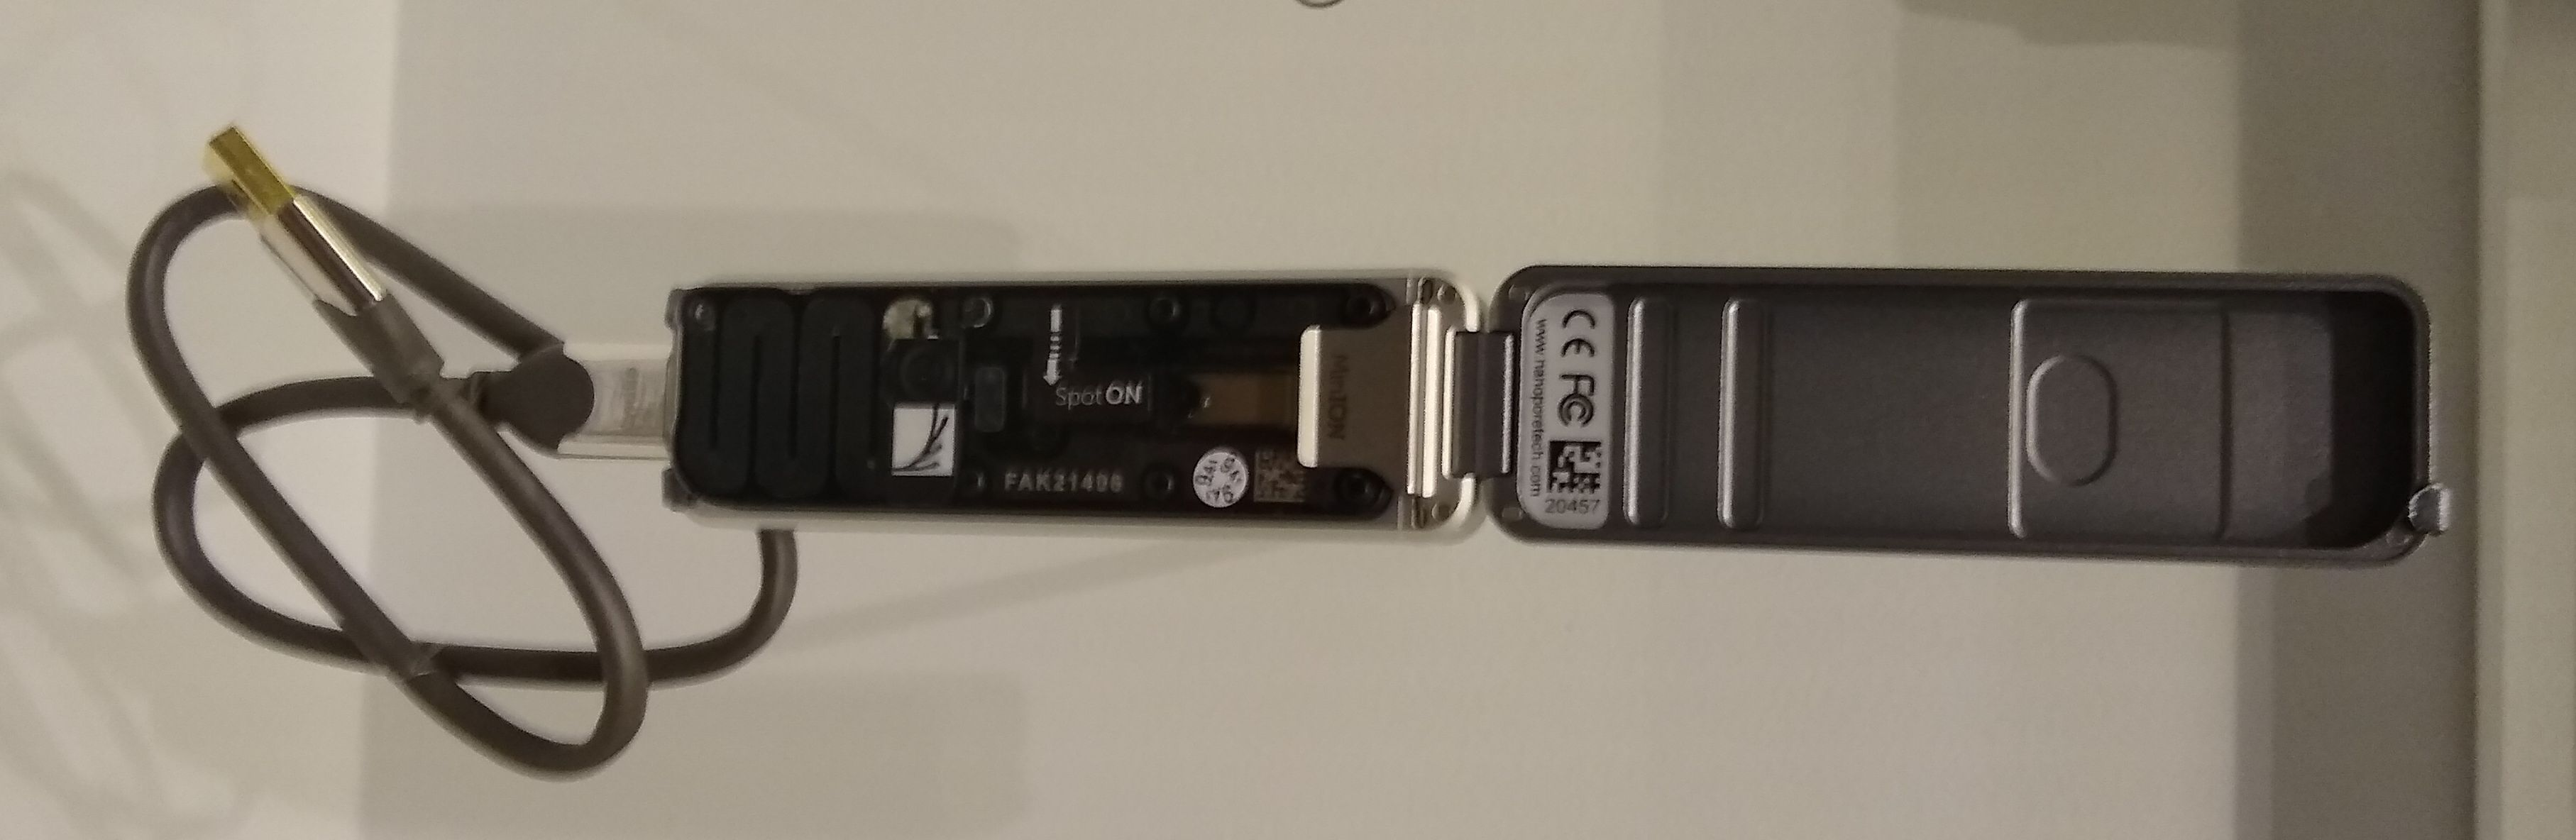
\includegraphics[width=0.7\linewidth]{files/MinionSequencer-c61d8c96564470a49494d3e2f2737064.jpg}
\caption[]{Oxford Nanopore MinION sequencer
Credits: \href{https://creativecommons.org/licenses/by-sa/4.0}{CC BY-SA 4.0} \cite{minion_2020}}
\label{minion}
\end{figure}

\begin{framed}
\textbf{Box 5.6: Nanopore sequencing}\\
The flow-cell in nanopore sequencing has a number
of wells. Each of these wells has a sensor at the bottom that detects
currents. The well itself is covered by a membrane, similar to a cell
membrane, although in this case it is not a lipid bilayer but a more stable
polymer. Embedded in this membrane are transmembrane protein pores
(genetically modified to work optimally) through which a DNA molecule fits.
A current potential is applied between the top and the bottom of the
membrane and, as DNA is negatively charged, it wants to travel through the
pore. This changes the electrical resistance, which is detected by the
sensor. A problem is that the DNA travels too fast for the sensor to detect
the nucleotides; the solution is to add a DNA-polymerase, that acts as a
brake (it is also called motor, as it actively unzips the DNA).
The polymerase itself does not fit through the pore and sits on top of it.

As with PacBio, the read length is determined by the input DNA fragment size
and has no theoretical limit: the current read length record stands at 4.2
Mb, which is enough to sequence a bacterial genome in a single read. Nanopore
sequencing has a similar error model as PacBio, with insertions and
deletions most prevalent. In addition to that, long stretches of homopolymers
remain challenging. Accuracy is limited to between 85 and 95\%, however the latest
duplex-calling (were both the template and the complement strand are read) reaches
99\% accuracy (Q20). The main advantage over any of the other
technologies is that the template DNA itself is measured, so base
modifications like DNA methylation can be detected as well. The sequencer
is also small enough to fit in the palm of a hand and people have used it in various
non-traditional conditions, such as arctic expeditions on Svalbard and in
the International Space Station.
\end{framed}

\begin{framed}
\textbf{Important things to know about nanopore sequencing}\\
\begin{itemize}
\item it can sequence very long reads
\item the accuracy is 98-99.9\% (Q17-Q30)
\item it can directly detect base modifications (methylation)
\item fragments with extreme GC content can be sequenced as there is no PCR step
\item individual DNA fragments are sequenced one after the other, making it real-time
\item it is a high throughput technology, with one flowcell yielding between 2.5 and 3.5 million reads (MinION)
\item good for genome assembly
\end{itemize}
\end{framed}

\subparagraph{Quality control}

\begin{figure}[!htbp]
\centering
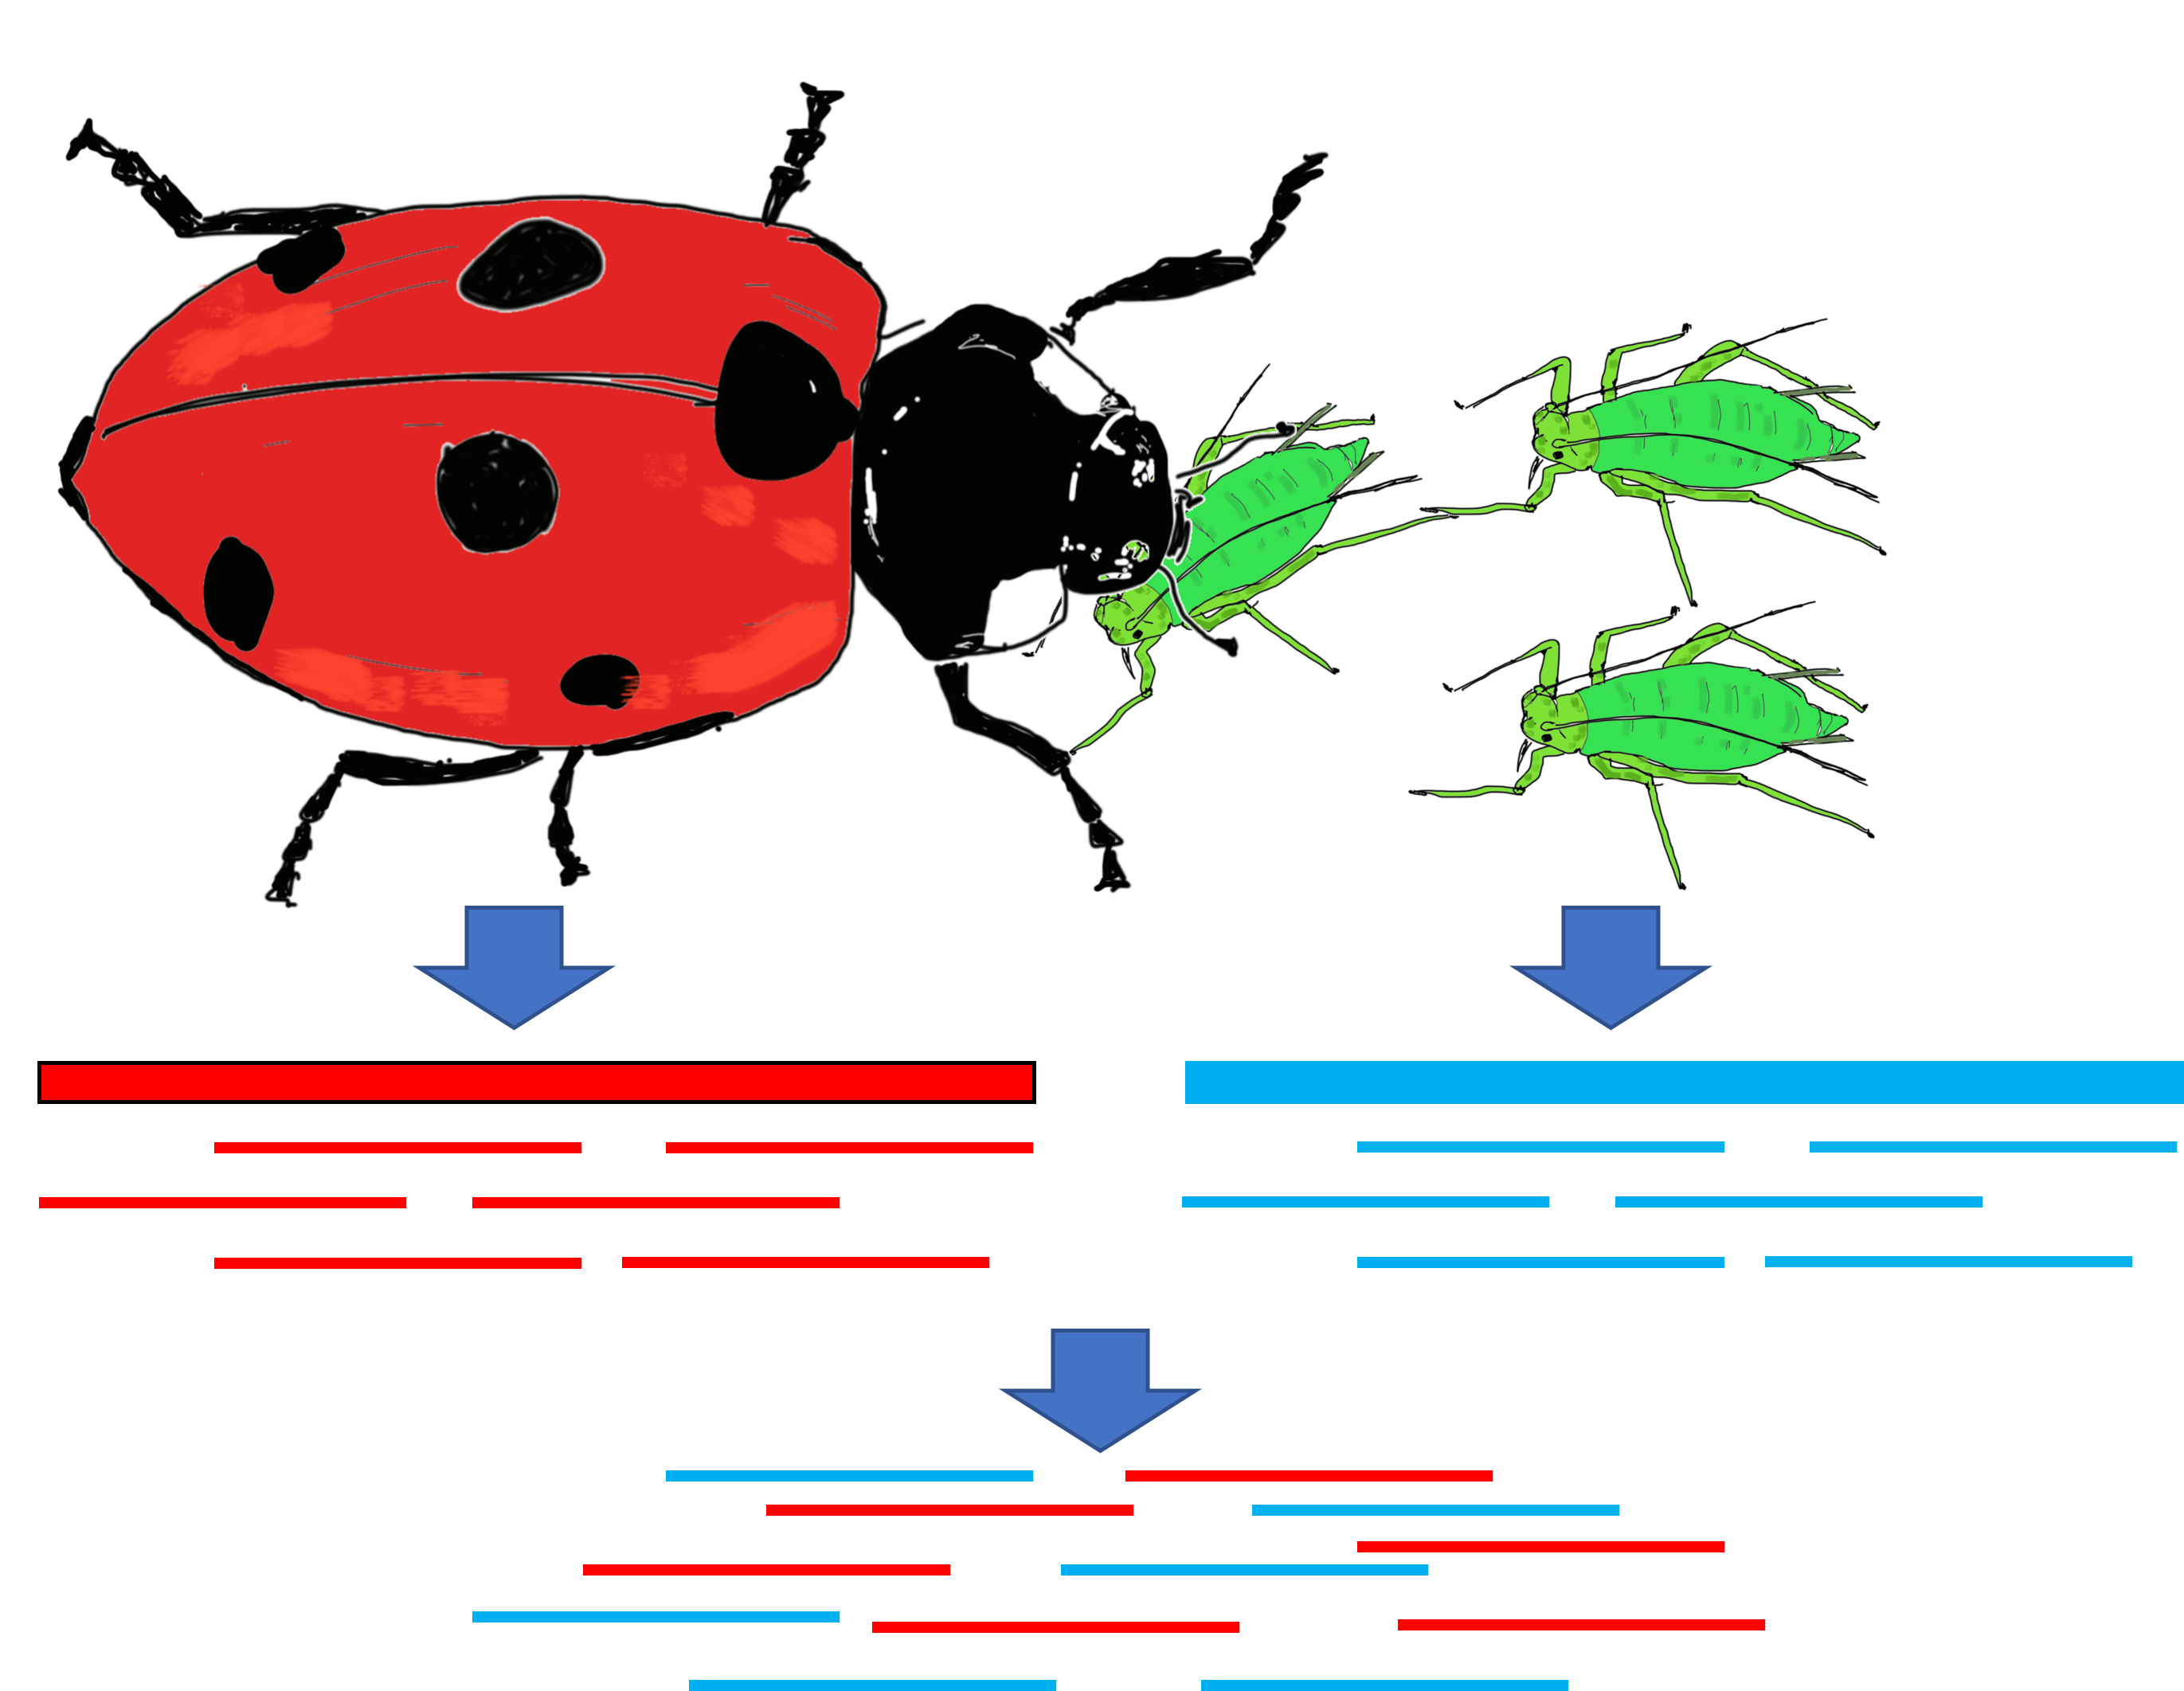
\includegraphics[width=0.375\linewidth]{files/ladybug_aphid-e54c4e12cd9d0b444a0b46651fd5915f.png}
\caption[]{Causes for contaminated sequencing \newline
samples, using as example the ladybug \newline
and its main food source, aphids. \newline
Credits: \href{https://creativecommons.org/licenses/by-nc/4.0/}{CC BY-NC 4.0} \cite{own_5_2024}}
\label{ladybug_aphid}
\end{figure}

As discussed above, sequencing technology is not perfect and errors will be
present in the output. Moreover, what we sequence is not always what we
originally intended to sequence (Figure~\ref{ladybug_aphid}).

Sources of errors related to sequencing itself are base calling errors
(substitution errors), uncalled bases (indels), GC bias, homopolymers, a
drop of quality towards the 3'end of a read, and duplicates (amplification
bias). Additional error sources are contamination of the input sample,
remnants of adapters and sequencing vectors. It is therefore important to
assess the quality of the sequencing itself and the output data before
further analysis.


\bigskip
\centerline{\rule{13cm}{0.4pt}}
\bigskip

\subparagraph{Genome assembly}

When no reference genome is available for a species, we need to assemble
one, i.e. build one from scratch by putting together DNA sequence reads.
Here we discuss what to do when a reference genome sequence is not yet
available. First, we examine why we would want to create a reference
assembly, and what types of references can be created. Next, the assembly
process and its challenges are introduced. Finally, genome annotation and
detection of structural variation are discussed.


\bigskip
\centerline{\rule{13cm}{0.4pt}}
\bigskip

\subparagraph{Reference genome quality}\label{chapter5_reference_genome_quality}

\begin{figure}[!htbp]
\centering
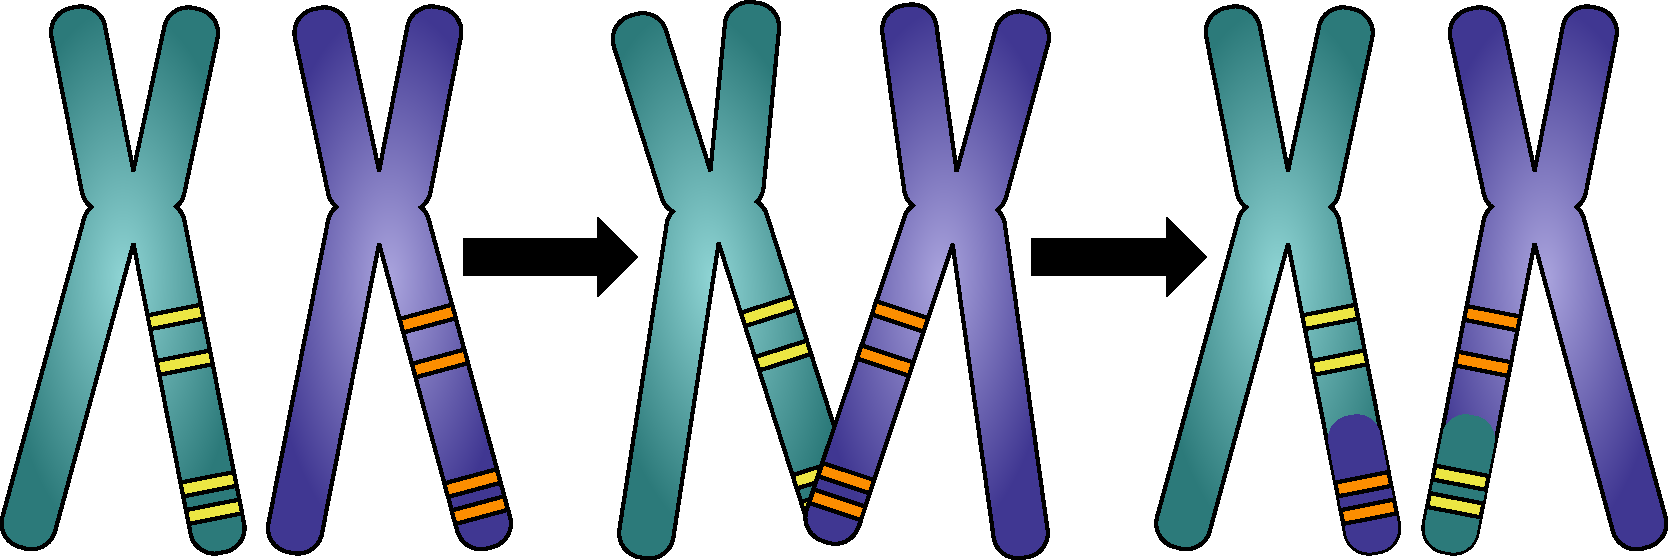
\includegraphics[width=0.375\linewidth]{files/co-segregation_alt-be606caac3ebd964dddd0b776d6326c8.pdf}
\caption[]{Co-segregation of alleles. \newline
Credits: \href{https://creativecommons.org/licenses/by-nc/4.0/}{CC BY-NC 4.0} \cite{own_5_2024}}
\label{co_segregation_alt}
\end{figure}

Genomes can be reconstructed with different aims, which influence the
required quality of the final assembly. The human genome, for example, has
been assembled as far as possible and in 2021, the first telomere-to-telomere
assembly was published, adding the final 5\% of
bases. It has taken enormous effort, both in terms of finance and labour,
to get to this stage. This is neither feasible nor strictly necessary for
each genome assembly project. Hence, most genome assemblies currently
available are so-called draft assemblies, and most fully completed genomes
are from bacteria and other species with small genomes. In terms of the
assembly process, for eukaryotic genomes the euchromatic regions assemble
best. Fortunately, these regions contain most of the genes, making draft
assemblies useful for studying mutations or expression patterns. When we
want to study larger features of the genome itself however, such as
co-segregation of alleles (Figure~\ref{co_segregation_alt}) or gene order (Figure~\ref{salmonella_alt}),
we need more contiguous assemblies. 3rd generation sequencing, scaffolding
and newer technologies such as chromatin conformation capture (Hi-C) etc.
make chromosome-level assemblies increasingly attainable.

\begin{figure}[!htbp]
\centering
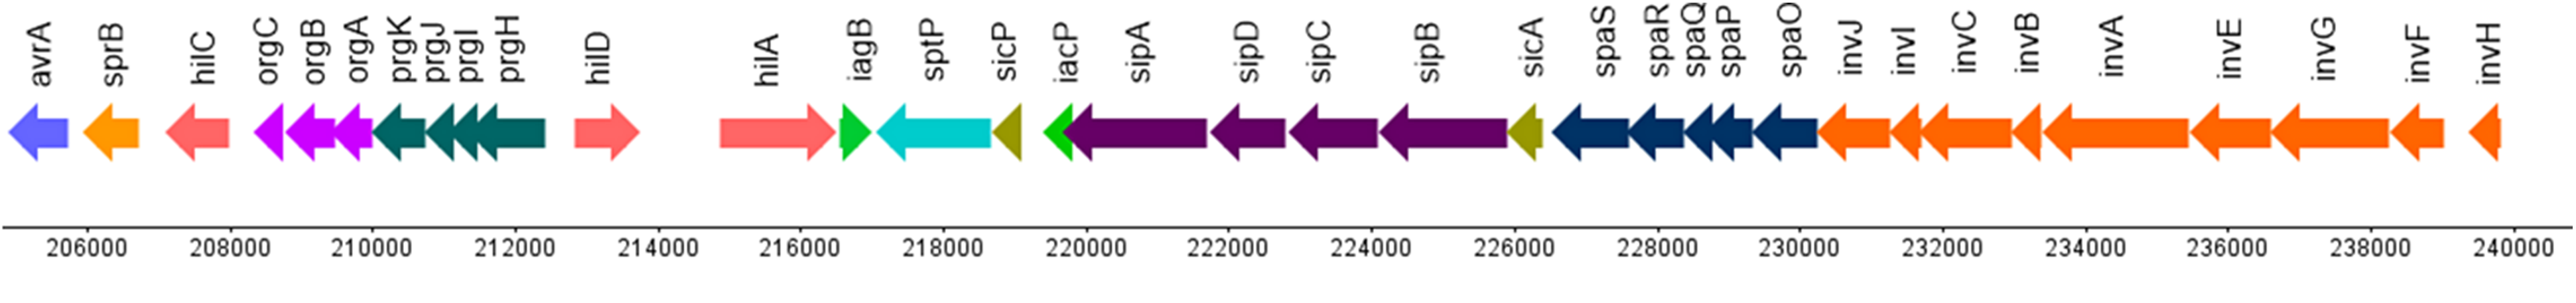
\includegraphics[width=0.7\linewidth]{files/salmonella_alt-bd73277b95307f2b3c81dbcb06f1536e.png}
\caption[]{Genetic representation of the \textit{Salmonella enterica subsp. enterica} serovar Stanley pathogenicity island-1.
Credits: \href{https://creativecommons.org/licenses/by/4.0/}{CC BY 4.0} modified from \cite{salmonella_alt_2019}.}
\label{salmonella_alt}
\end{figure}


\bigskip
\centerline{\rule{13cm}{0.4pt}}
\bigskip

\subparagraph{Genome assembly strategies}

In the early days of DNA sequencing, generating sequencing reads was very
costly. Much effort was therefore spent on developing methods requiring a
minimum amount of sequence data to assemble a genome. Moreover, Sanger
sequencing requires all fragments of DNA in a run to be identical, so some
form of organising the DNA was required. This was initially done by
sequencing the start of a single large fragment (much longer than the read
length), and generating sequencing primers from the end of the sequenced
part for the next round of sequencing, until the end of the fragment was
reached. This rather tedious approach was not feasible for larger genomes.
This led to the development of the whole genome shotgun sequencing method,
made possible by the growth in compute power for assembly. With the advent
of 2nd generation sequencing, this was updated by leaving out the cloning
step. 2nd generation sequencing technology (e.g. Illumina) allows for a
mixture of fragments to be sequenced at the same time and the volume of
sequencing data generated is large. So instead of requiring lab work to
select which section to sequence, everything is sequenced at once and the
puzzle is solved later by computer.


\bigskip
\centerline{\rule{13cm}{0.4pt}}
\bigskip

\subparagraph{Whole genome sequencing}

Nowadays, the most widely employed genome sequencing approach is whole
genome sequencing (WGS, Figure~\ref{WGS}). As the term implies the whole
genome is sequenced, without discrimination. DNA is extracted from cells
and sheared into random fragments. These fragments are then size selected
and sequenced using Illumina, PacBio or Oxford Nanopore technology. Note
that WGS generally generates draft genome assemblies; additional steps are
required to gain a complete, high-quality reference genome assembly.

\begin{figure}[!htbp]
\centering
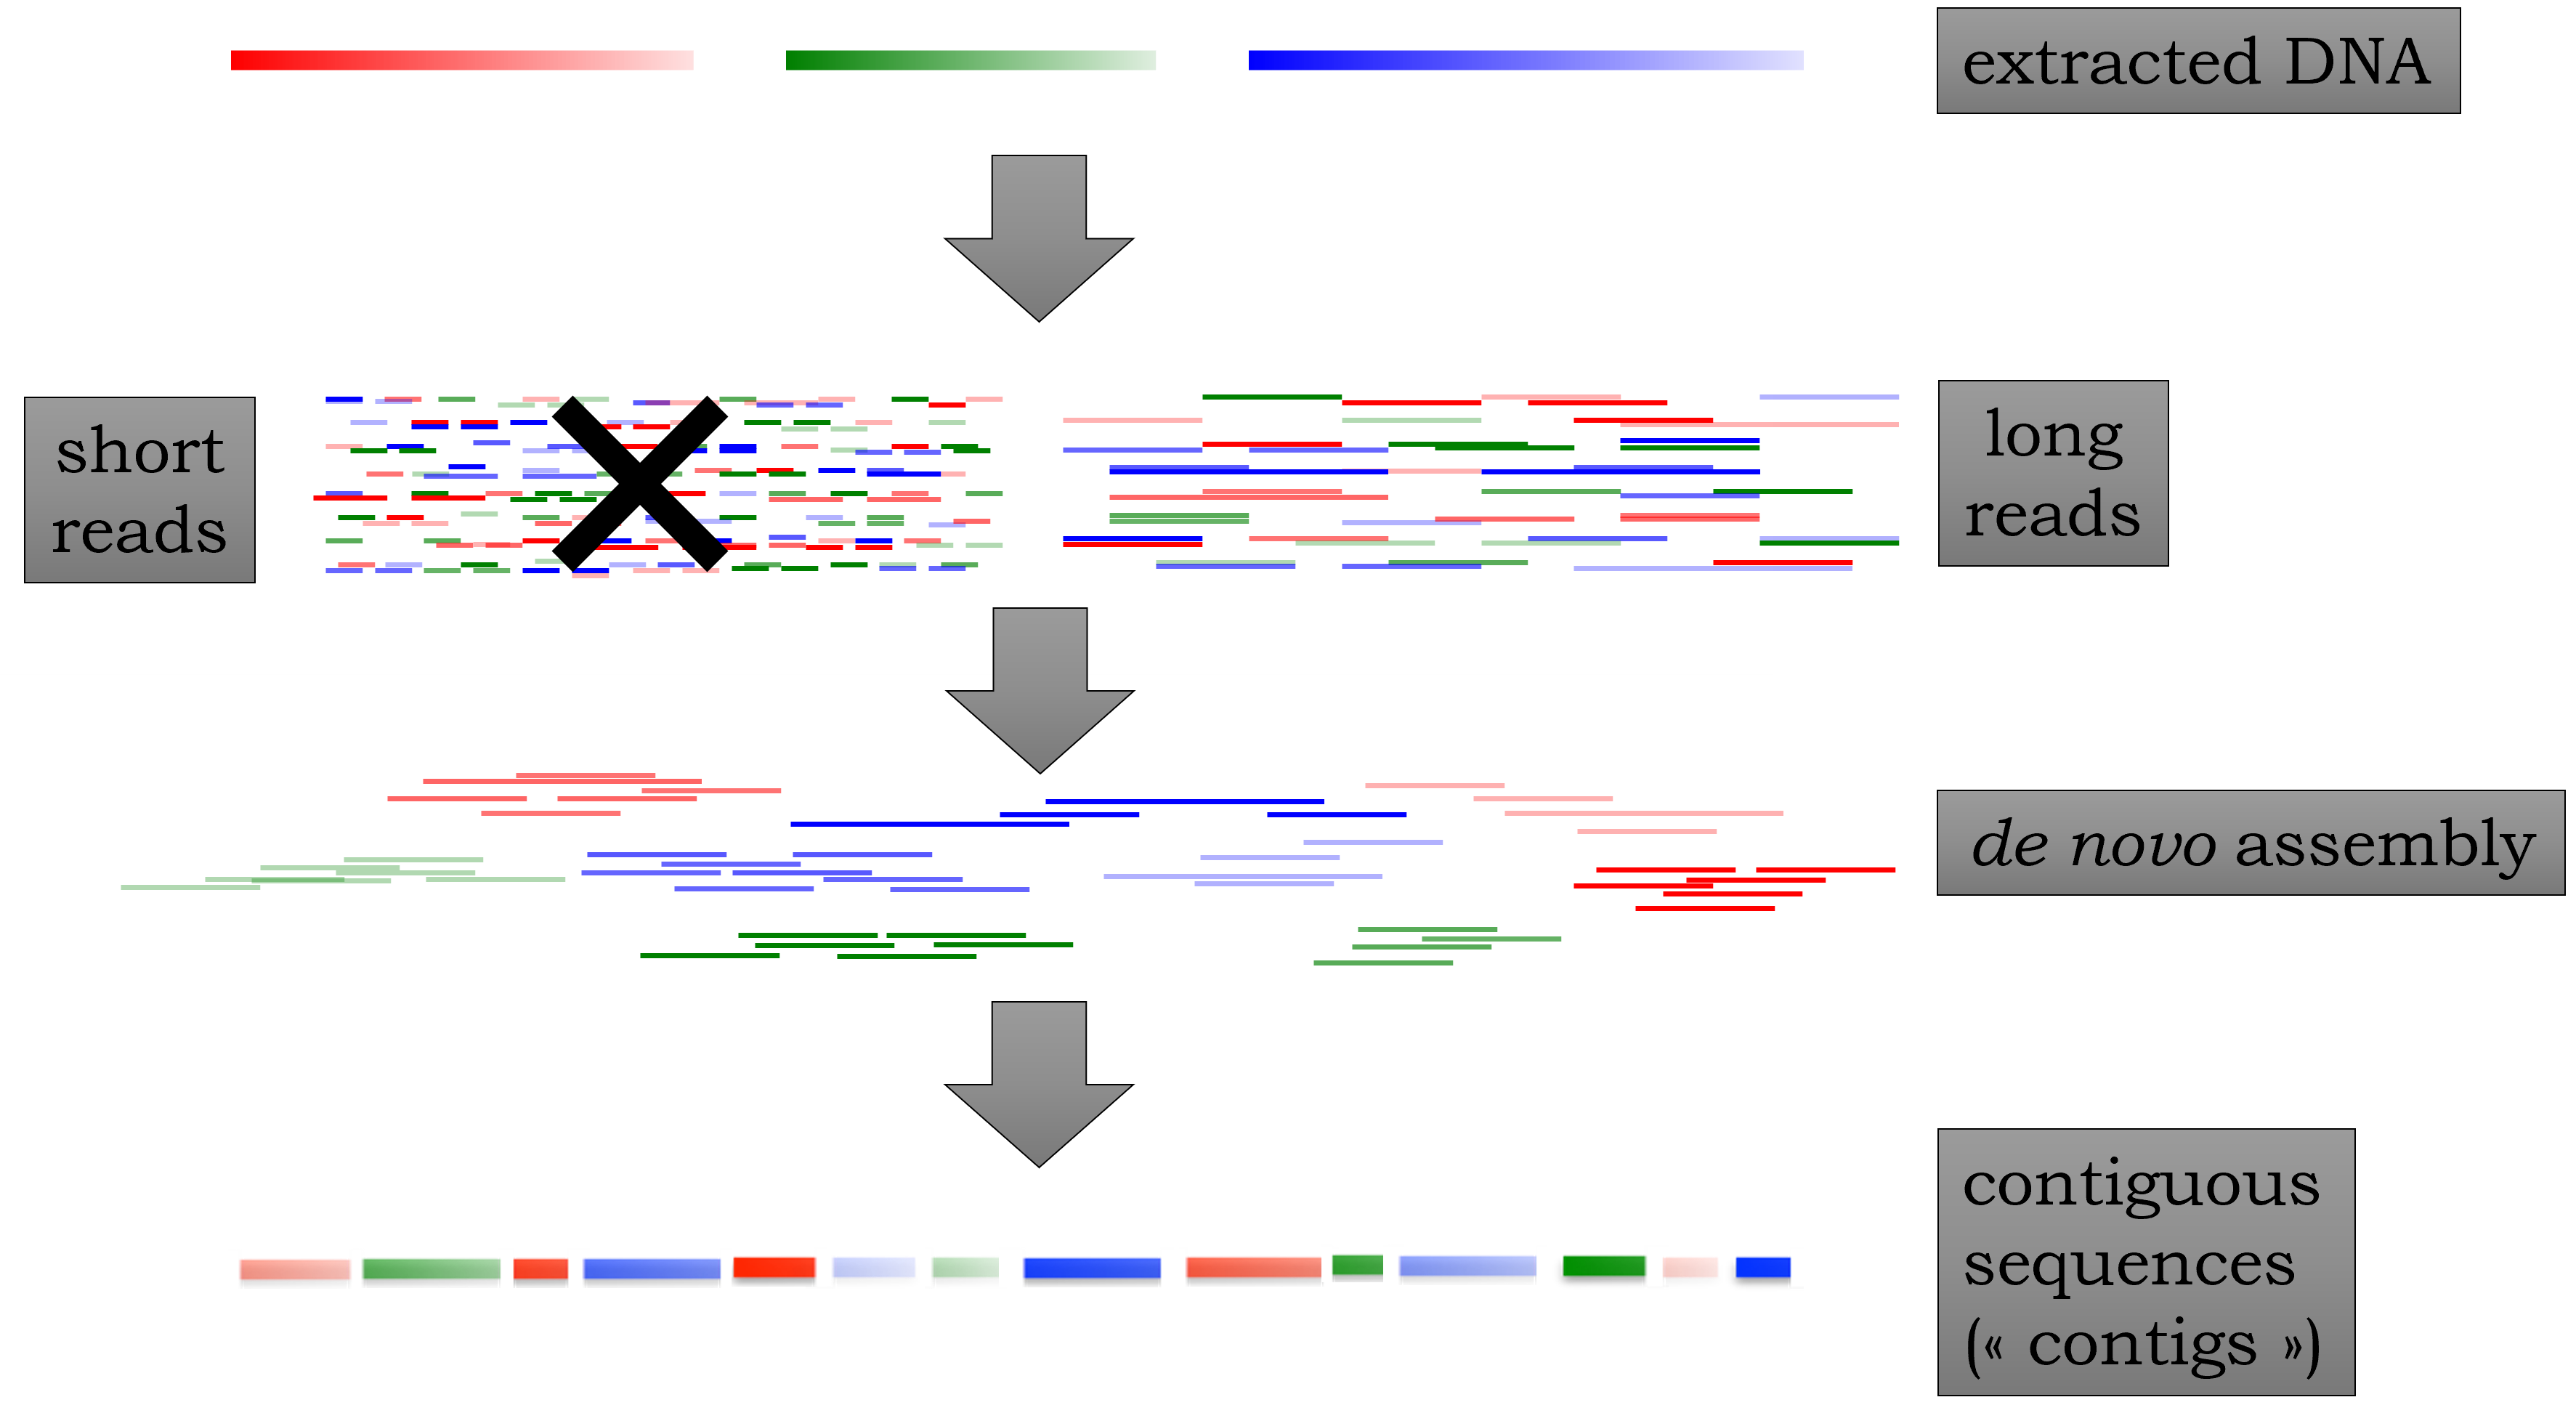
\includegraphics[width=0.7\linewidth]{files/genome_assembly-b423f2edbcdd981df9c73980589a8dd7.png}
\caption[]{Whole genome sequencing and assembly. \newline
Short reads on the left are generally not used anymore for \textit{de novo} assembly. \newline
Credits: \href{https://creativecommons.org/licenses/by-nc/4.0/}{CC BY-NC 4.0} \cite{own_5_2024}}
\label{WGS}
\end{figure}


\bigskip
\centerline{\rule{13cm}{0.4pt}}
\bigskip

\subparagraph{Assembly challenges}

The main challenge of assembly is to reconstruct the original genome
sequence from the millions or billions of small fragments. Some people have
likened this process to putting a stack of newspapers (each newspaper
representing one copy of the genome) through a shredder and attempting to
reconstruct a single original newspaper from the resulting confetti.
Solving this puzzle has driven the development of dedicated assembly
algorithms and software. Any computational approach has to overcome the
real-world challenges posed by the sequenced data and the characteristics of
genomes.

\begin{figure}[!htbp]
\centering
\includegraphics[width=0.7\linewidth]{files/fish_puzzle_numbers-027345da91885e2888e0af6f935ddca4.png}
\caption[]{The assembly problem as a jigsaw puzzle. Numbers are referred to in the text.
Credits: Based on \href{https://creativecommons.org/public-domain/pdm/}{Public Domain Mark} \cite{three_fish}, \href{https://creativecommons.org/licenses/by-nc/4.0/}{CC BY-NC 4.0} \cite{own_5_2024}.}
\label{jigsaw}
\end{figure}

If we look at a genome assembly using the analogy of a jigsaw puzzle (Figure~\ref{jigsaw}), the challenges become obvious:

\begin{itemize}
\item There is no picture on the puzzle box, i.e. we have no idea what the assembled genome is meant to look like.
We can look at related genomes, but this will only give an approximate idea. (Number 1 in the image)


\item There are loads of pieces in the puzzle, billions of them.
Every piece represents a small part of the genome that has been sequenced.


\item Some pieces are frayed or dirty, i.e., reads contain errors, further obfuscating the overall picture. (2 and 5)


\item Some pieces are missing.
Some parts of the genome do not break as easily as others, and are not included in the sheared fragments.
Other have extreme GC values and do not amplify as well in the PCR step. (3)


\item Some parts of the puzzle contain the same image.
In genome terms, these are duplicated regions, where some genes may have more than one copy.
For example, the ribosomal RNA cistron (the region which encodes the parts of the ribosome) consists of multiple copies. (4)


\item Some parts of the puzzle look completely identical and are featureless: the repeat regions. (6)


\item In circular genomes, there are no ``corners'': we do not know where the genome begins or ends. (7)
\end{itemize}

In addition to the metaphors of the single puzzle, many organisms contain
two (i.e. diploid) or more (i.e. polyploid) copies of the same chromosome,
with small differences between them. In essence, in this case we try to
assemble one puzzle from two (or more) slightly different versions. If
these differences grow too big, parts from the two puzzles may be assembled
independently without noticing (remember - we have no puzzle box!).

With long high-quality reads this puzzle challenge becomes simpler, as there
are fewer pieces in total and fewer featureless parts. Currently,
chromosome-level assemblies are routinely generated using PacBio HiFi reads
in combination with Hi-C.


\bigskip
\centerline{\rule{13cm}{0.4pt}}
\bigskip

\subparagraph{Repeats}

Repeat regions (i.e., the boring background) are the main challenge in genome
assembly and most contigs (contiguous sequences, the longest stretches that
can be assembled unequivocally) stop at the edges of repetitive regions.
The process is like finding many puzzle pieces containing both bits of fish
and background, and trying to figure out which edge belongs to which fish and
how much background goes in between. One solution for solving the repeat
problem are longer reads (that can bridge the sea between two fishes).
To illustrate the scale of the problem that repeats pose in assembly: most
mammalian Y-chromosomes have not been assembled for more than 50\%, because
of the repeat content.
Chapter~1 explains how to mask repeats from a genome
as a first step prior to genome annotation.


\bigskip
\centerline{\rule{13cm}{0.4pt}}
\bigskip

\subparagraph{Assembly quality assessment}

When assembling a new genome, we have no way of verifying its quality
against a known ground truth. We also rarely get a complete genome or
chromosome as a single contig or scaffold as a result. Therefore, other
metrics and methods are required to assess the quality of an assembly. We
can use the experience gained in other assembly projects to gauge the
quality of an assembly; we can compare it to closely related genomes that
have already been assembled; and we can compare the assembly with the
expectations we have about the genome in terms of overall size, number of
chromosomes and genes, given the known biology of the species.


\bigskip
\centerline{\rule{13cm}{0.4pt}}
\bigskip

\subparagraph{Structural and functional annotation}

The next step after genome assembly is annotation. First, during
structural annotation we try to identify the location and structure of
(protein coding) genes (\textit{see} chapter~1~-~Gene~prediction).
Next, we attempt to identify the function of the predicted gene during functional
annotation (\textit{see} chapter~1~-~Functional~annotation).


\bigskip
\centerline{\rule{13cm}{0.4pt}}
\bigskip

\subparagraph{Insights from complete genomes}

The contiguity and completeness of an assembly determines what we can learn
from them. In the reference~genome~quality section, co-segregating alleles and gene
order were already mentioned. If a genome is assembled in fewer, larger
pieces (i.e., longer contigs), we can also understand more about the long
distance regulatory elements that play a role in regulation of gene
expression (Figure~\ref{Pax6_locus}).

\begin{figure}[!htbp]
\centering
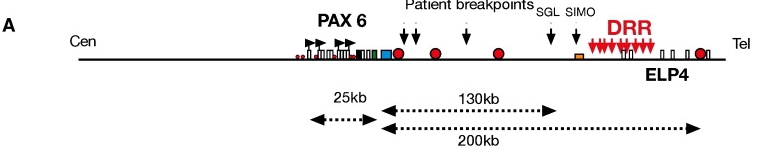
\includegraphics[width=0.7\linewidth]{files/Pax6_operon-35a0d631e476d83c9661af6593f2aec6.jpg}
\caption[]{Physical map of the human PAX6 locus showing long distance regulatory elements.
Credits: \cite{pax_locus}}
\label{Pax6_locus}
\end{figure}

As discussed above, the telomere-to-telomere assembly of the human genome
added the 5\% hitherto missing genome sequence. While the previous human
genome assembly was already considered gold standard and very complete, the
number of genes increased with 5\%, of which 0.4\% were protein coding. This
increase in identified genes also allows the study of expression patterns of
these genes. An increase in genome coverage can also reveal hidden
elements. As an illustration, Figure~\ref{FSHD} shows all paralogs of a disease related gene that
have finally been resolved. Most of the missing copies were in hard to
sequence parts of the genome. Chromosome-level assemblies also allow us to
study genome evolution itself, the way chromosomes are rearranged during
evolution and speciation.

\begin{figure}[!htbp]
\centering
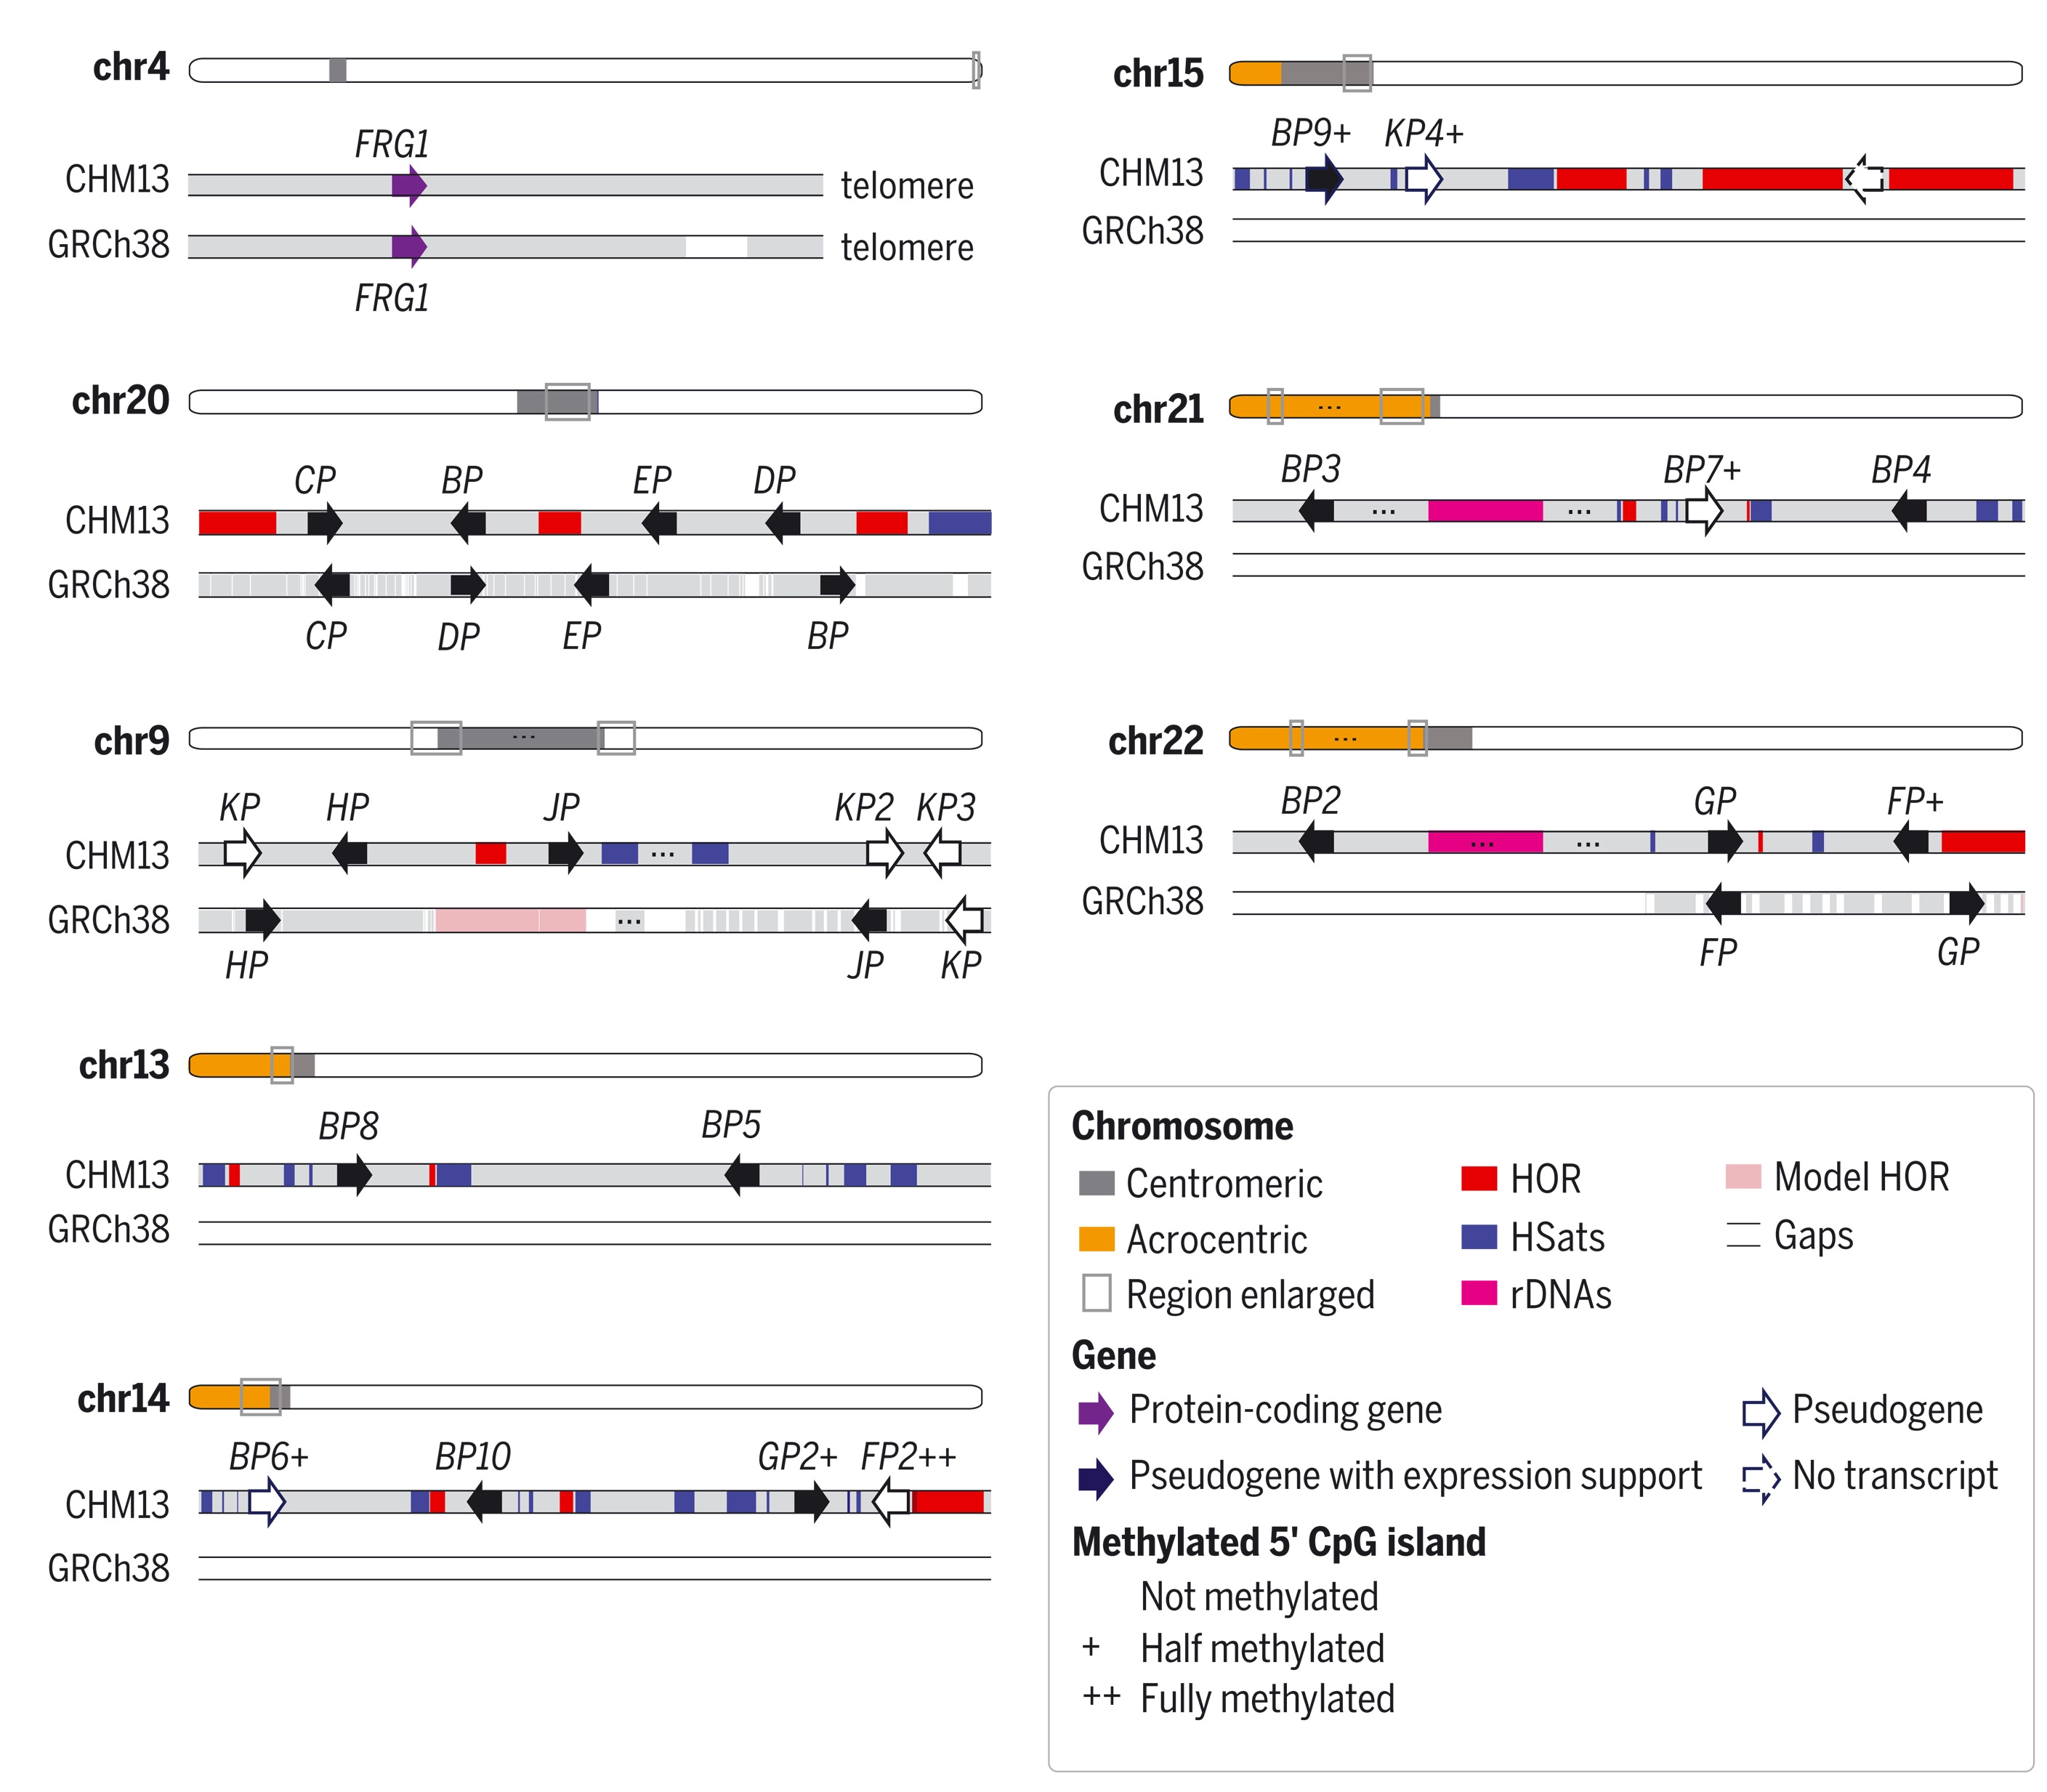
\includegraphics[width=0.7\linewidth]{files/FSHD-7029b8251fc4233c610d79d4d5b5cbc5.png}
\caption[]{The protein-coding gene \textit{FRG1} and its 23 paralogs in CHM13. Only 9
were found in the previous assembly (GRCh38). Genes are drawn larger than
their actual size, and the ``\textit{FRG1}'' prefix is omitted for brevity. All
paralogs are found near satellite arrays. \textit{FRG1} is involved in
acioscapulohumeral muscular dystrophy (FSHD).
Credits: modified from \href{https://creativecommons.org/licenses/by/4.0}{CC BY  4.0} via PMC \cite{t2t_human_genome_2022}.}
\label{FSHD}
\end{figure}


\bigskip
\centerline{\rule{13cm}{0.4pt}}
\bigskip

\begin{framed}
\textbf{Box 5.7: Phenotypic variation}\\
Small variants can have large phenotypic effects.

\begin{figure}[!htbp]
\centering
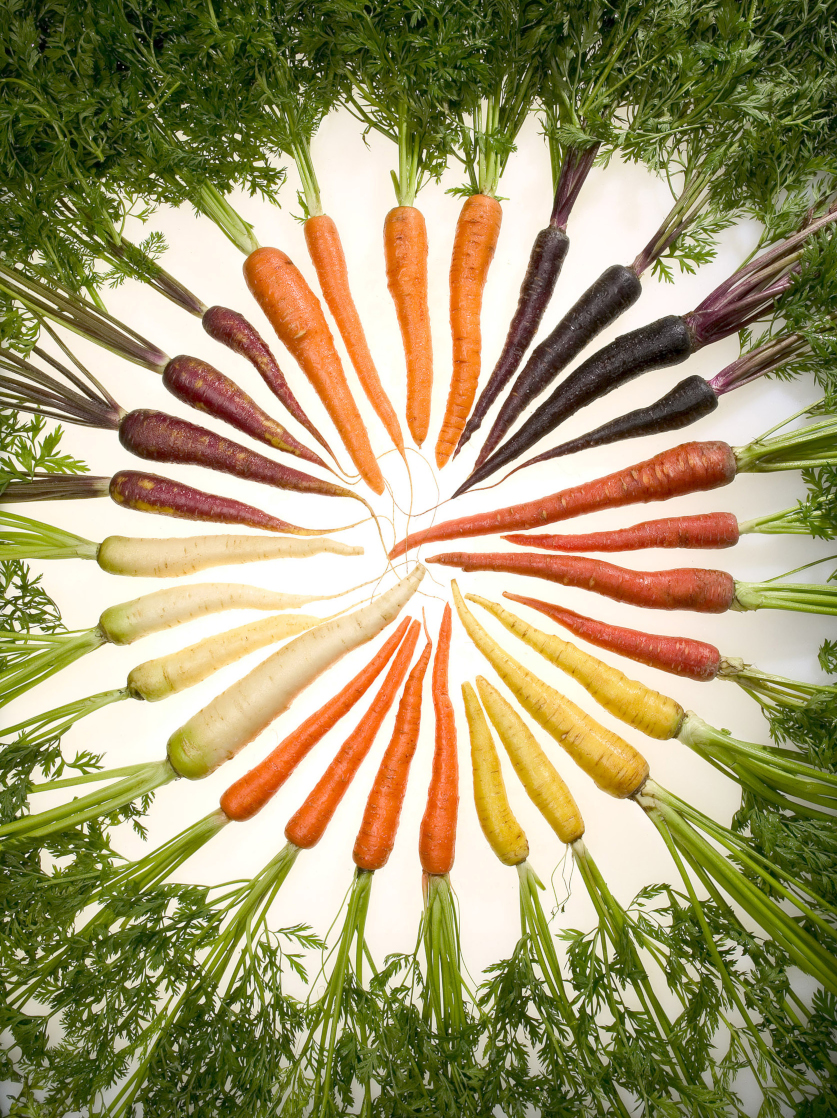
\includegraphics[width=0.25\linewidth]{files/carrots-c58b6efdae05aa74dcdaa9a4c1da4f00.jpg}
\caption[]{Colour variations in carrots. \newline
Credits: \href{https://creativecommons.org/publicdomain/zero/1.0/}{CC0 1.0} \cite{carrots_2006}.}
\label{carrots}
\end{figure}

They account for the observable variation in things all around us. In
agriculture, variants have been actively selected for to create the wide
varieties of shapes, color and taste we see in our food items today (Figure~\ref{carrots}).
Historically, variants have been selected purely on these visible phenotypes
and new ones have been created mainly by chance in large-scale crosses.

Nowadays genetic information obtained through genome sequencing and variant
calling is used more and more in plant and animal breeding and selection.
\end{framed}

\paragraph{Variants}\label{chapter5_variants}

When a (nearby) reference genome is already available, reads can also be
mapped to that genome. Mapping entails finding the location in the genome
that matches each read, allowing for some small differences - genomic variation. Such variation can help
explain phenotypic variation (see Box~5.3). Genomic variation
between samples, individuals, and/or species can also be used to study
evolutionary history (see also chapters \href{/chapter2}{2} and \href{/chapter3}{3}, on multiple sequence
alignments and phylogeny).

% #% Add direct cross-link to MSA in chapter 2 when written.

Variants are divided into two main groups: structural or large-scale
variants and small-scale variants. First, we will focus on small-scale variants.
Within this group we distinguish single-nucleotide polymorphisms (SNPs),
multiple nucleotide polymorphisms (MNPs) and small insertions and deletions
(indels):

\begin{figure}[!htbp]
\centering
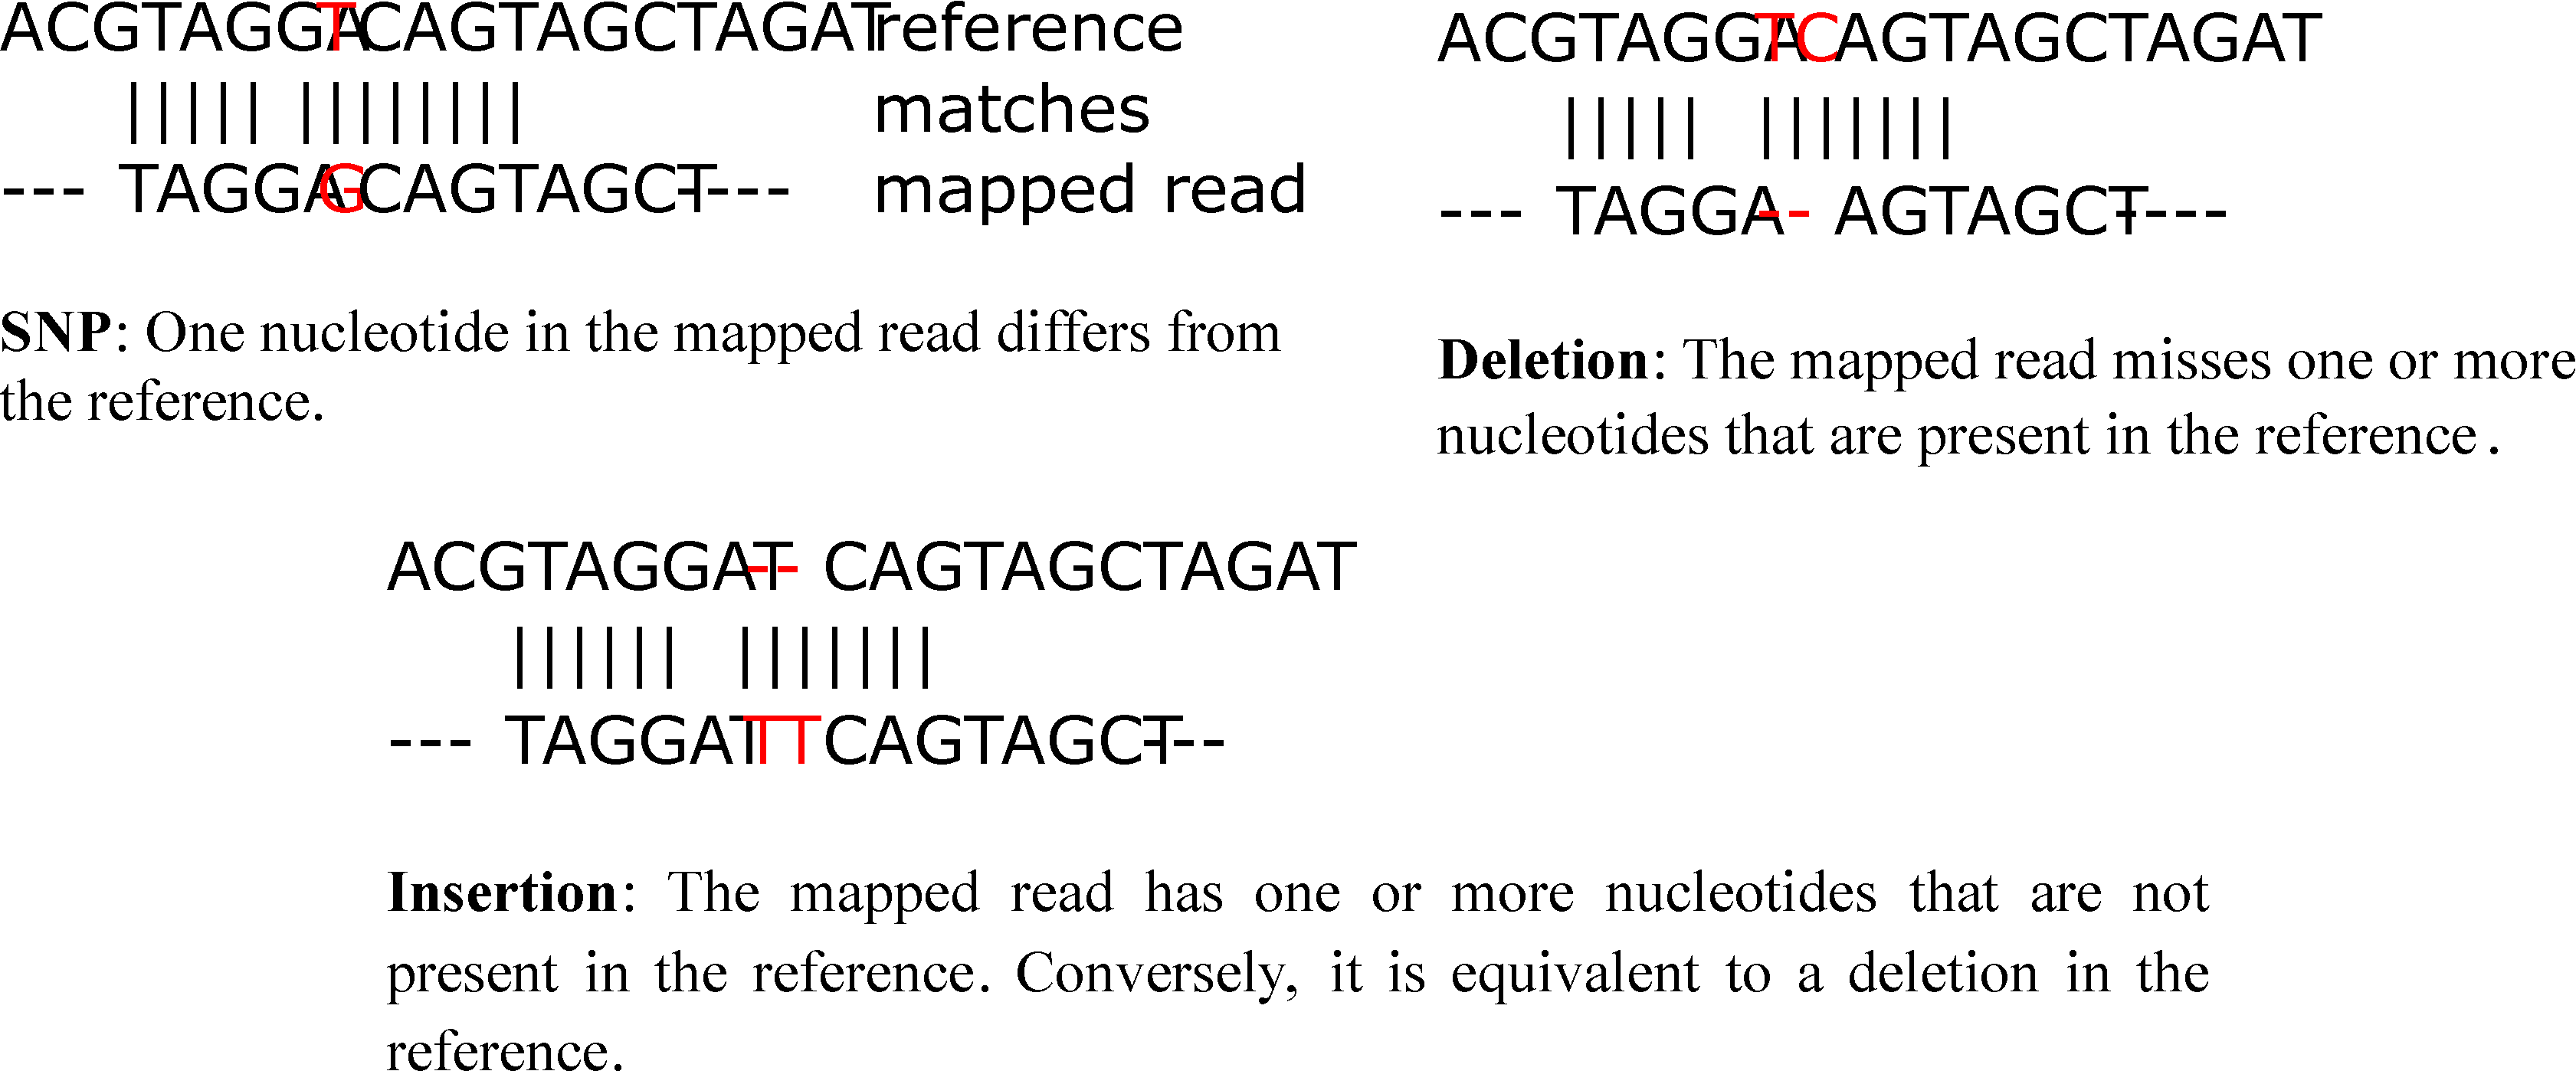
\includegraphics[width=0.7\linewidth]{files/indels-19dcc5ad970eccb0c1b8524aa32799d6.pdf}
\caption[]{A single-nucleotide polymorphism (top left), an insertion (bottom), and a deletion (top right).
Credits: \href{https://creativecommons.org/licenses/by-nc/4.0/}{CC BY-NC 4.0} \cite{own_5_2024}.}
\label{indels}
\end{figure}

Each variant at a particular position of a reference genome is called an
allele. In our example of an SNP above (Figure~\ref{indels}), we have a reference allele T and an
alternate allele G. When a sample originates from a single individual, the
theoretical number of alleles at any position of the reference cannot exceed
the ploidy of that individual: a diploid organism can at most have two
different alleles (as in our example), a tetraploid can at most have four,
etc. Given that we only have four different nucleotides, the maximum number
of possible alleles for a single position is four, for higher ploidy alleles
get complicated. But if we find more than two alleles in a diploid organism
it must be the result of an error, either in the read or in the reference.


\bigskip
\centerline{\rule{13cm}{0.4pt}}
\bigskip

\subparagraph{Variant calling}\label{chapter5_Variant_Calling}

As we have already seen, variants can be real, they can be the result of
sequencing errors, or represent errors in the reference sequence. The
process of detecting variants (SNPs and indels) and determining which are
real or most likely errors is called variant calling. To indicate the
probability that a variant is real, a quality score is assigned to each
variant. This considers the read depth and the mapping quality at the
position of a putative variant. Variant calling software will also report,
among a whole host of statistics, the so-called allele frequency (AF),
determined by the number of reads representing each allele that map. In a
diploid organism with one reference allele and one alternate allele we
expect both, on average, to have a frequency of 0.5. When the frequency of
one allele is close to 0, it is an indication that this variant is most
likely due to an error.


\bigskip
\centerline{\rule{13cm}{0.4pt}}
\bigskip

\begin{figure}[!htbp]
\centering
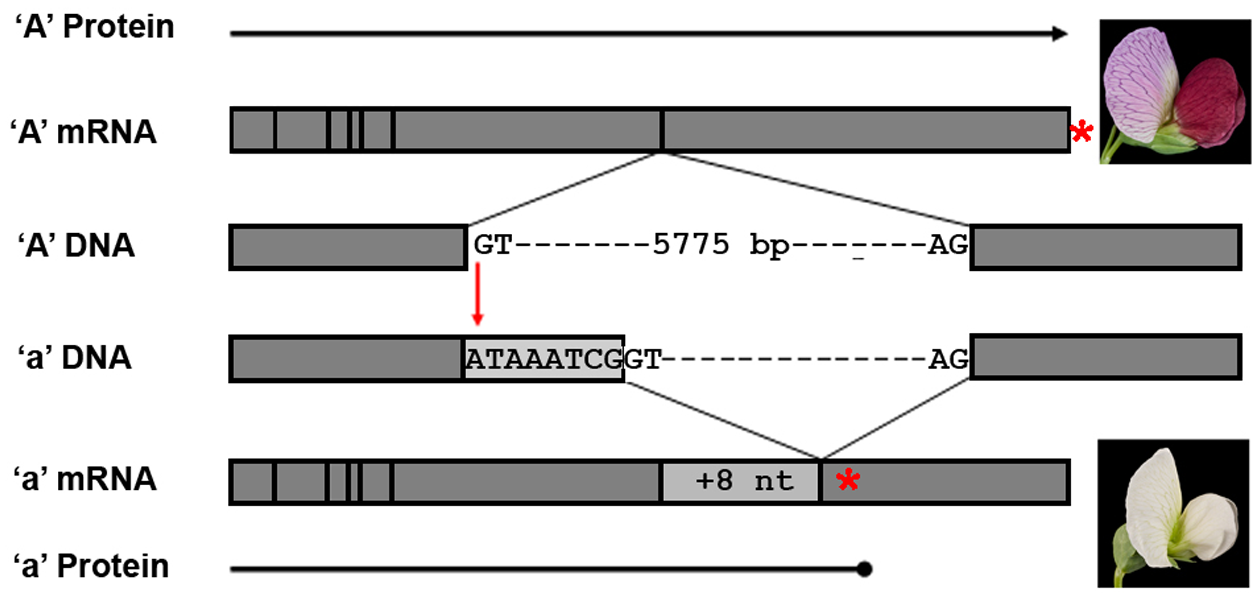
\includegraphics[width=0.7\linewidth]{files/flower-color-284df92adc23ba82dcd4d3e9841adaf7.png}
\caption[]{The main features of the \textit{bHLH} gene and its expression products (not to
scale). In Caméor, a white flowered pea cultivar of genotype \textit{a}, there is
a single G to A mutation in the intron 6 splice donor site that disrupts the
GT sequence required for normal intron processing. In the DNA, exons 6 and
7 are shown as grey boxes that flank the intron 6 splice donor and acceptor
sequences. In the RNA, the vertical lines represent exon junctions, and the
light grey box represents the 8 nucleotide (nt) insertion in the \textit{a} mRNA
that results from mis-splicing of intron 6. The red stars show the position
of the stop codon in the predicted protein, highlighting the premature
termination in the white flowered cultivar.
Credits: \href{https://creativecommons.org/publicdomain/zero/1.0/}{CC0 1.0} \cite{flower_color_2010}.}
\label{flower_color}
\end{figure}

\subparagraph{Variants and their effects}

SNPs between individuals underly most phenotypic variation. Sometimes a
single variant causes a different phenotype, like the classical mendelian
trait of flower color (Figure~\ref{flower_color}).  More often phenotypic traits are
the result of multiple variants, one example is height. Some variants can
cause hereditary defects or increase the risk of certain diseases.
Well-studied examples are mutations in the BRCA1 and BRCA2 genes
(Figure~\ref{BRCA_alt}). A specific mutation in the BRCA1 gene increases the
chance for that person to develop breast cancer during their lifetime to
80\%.

\begin{figure}[!htbp]
\centering
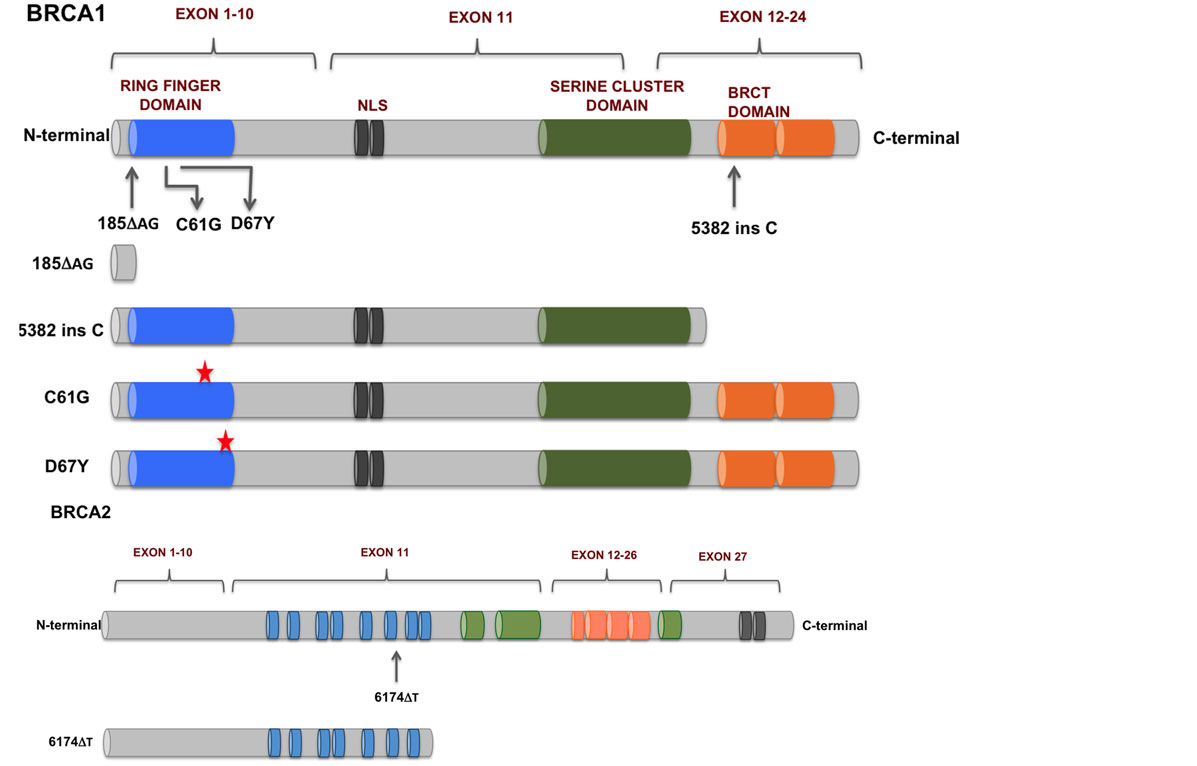
\includegraphics[width=0.7\linewidth]{files/BRCA_alt-25cc848b4877d5d349681d99d2a7cdd2.png}
\caption[]{Mutations in BRCA1 and BRCA2 found in breast and ovarian cancers.
Credits: \href{http://creativecommons.org/licenses/by/4.0/}{CC BY 4.0} \cite{BRCA_alt_2018}.}
\label{BRCA_alt}
\end{figure}


\bigskip
\centerline{\rule{13cm}{0.4pt}}
\bigskip

\subparagraph{Large-scale genome variation}

Above, we discussed small scale variants such as SNPs and indels. In
contrast, large-scale variants are structural variants where parts of
genomes have been rearranged, duplicated or deleted (Figure~\ref{large_scale_variants}). A
special case is copy number variation, where genes (or exons) have been
duplicated.

\begin{figure}[!htbp]
\centering
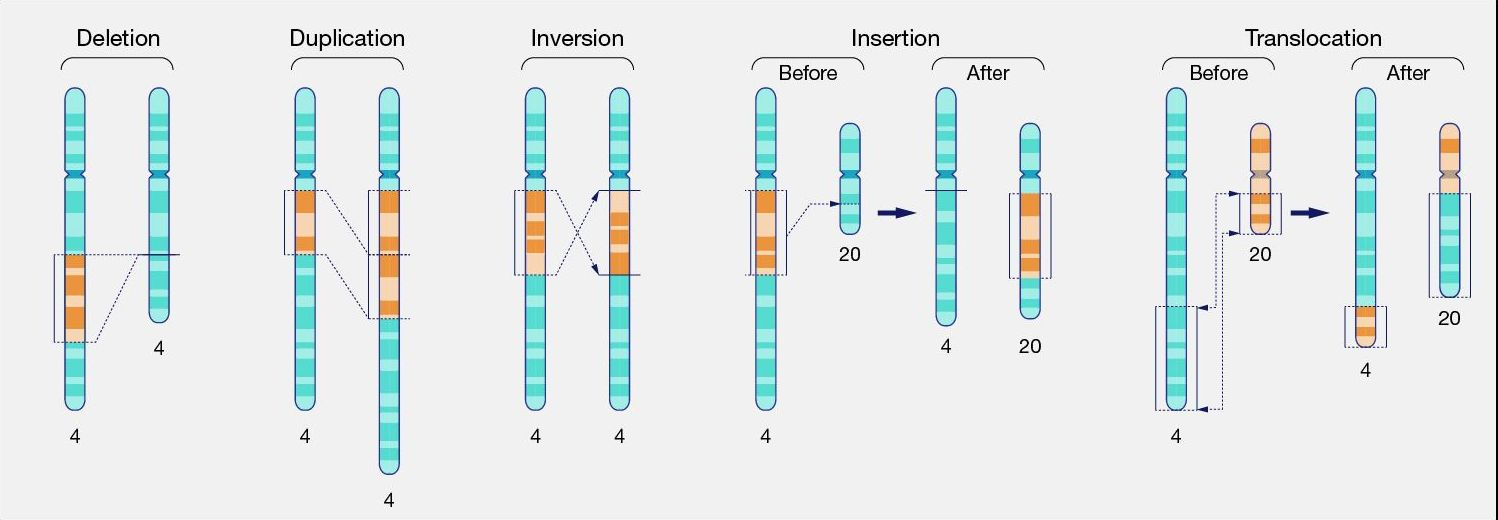
\includegraphics[width=0.7\linewidth]{files/large-scale-variants-a33e729252760d79b78ed291e2904c5d.jpg}
\caption[]{Different types of structural variants on chromosome level. Credits: \href{https://creativecommons.org/publicdomain/zero/1.0/}{CC0 1.0} \cite{large_scale_variants_2024}.}
\label{large_scale_variants}
\end{figure}

\begin{framed}
\textbf{Box 5.8: Cri du chat syndrome}\\
\begin{figure}[!htbp]
\centering
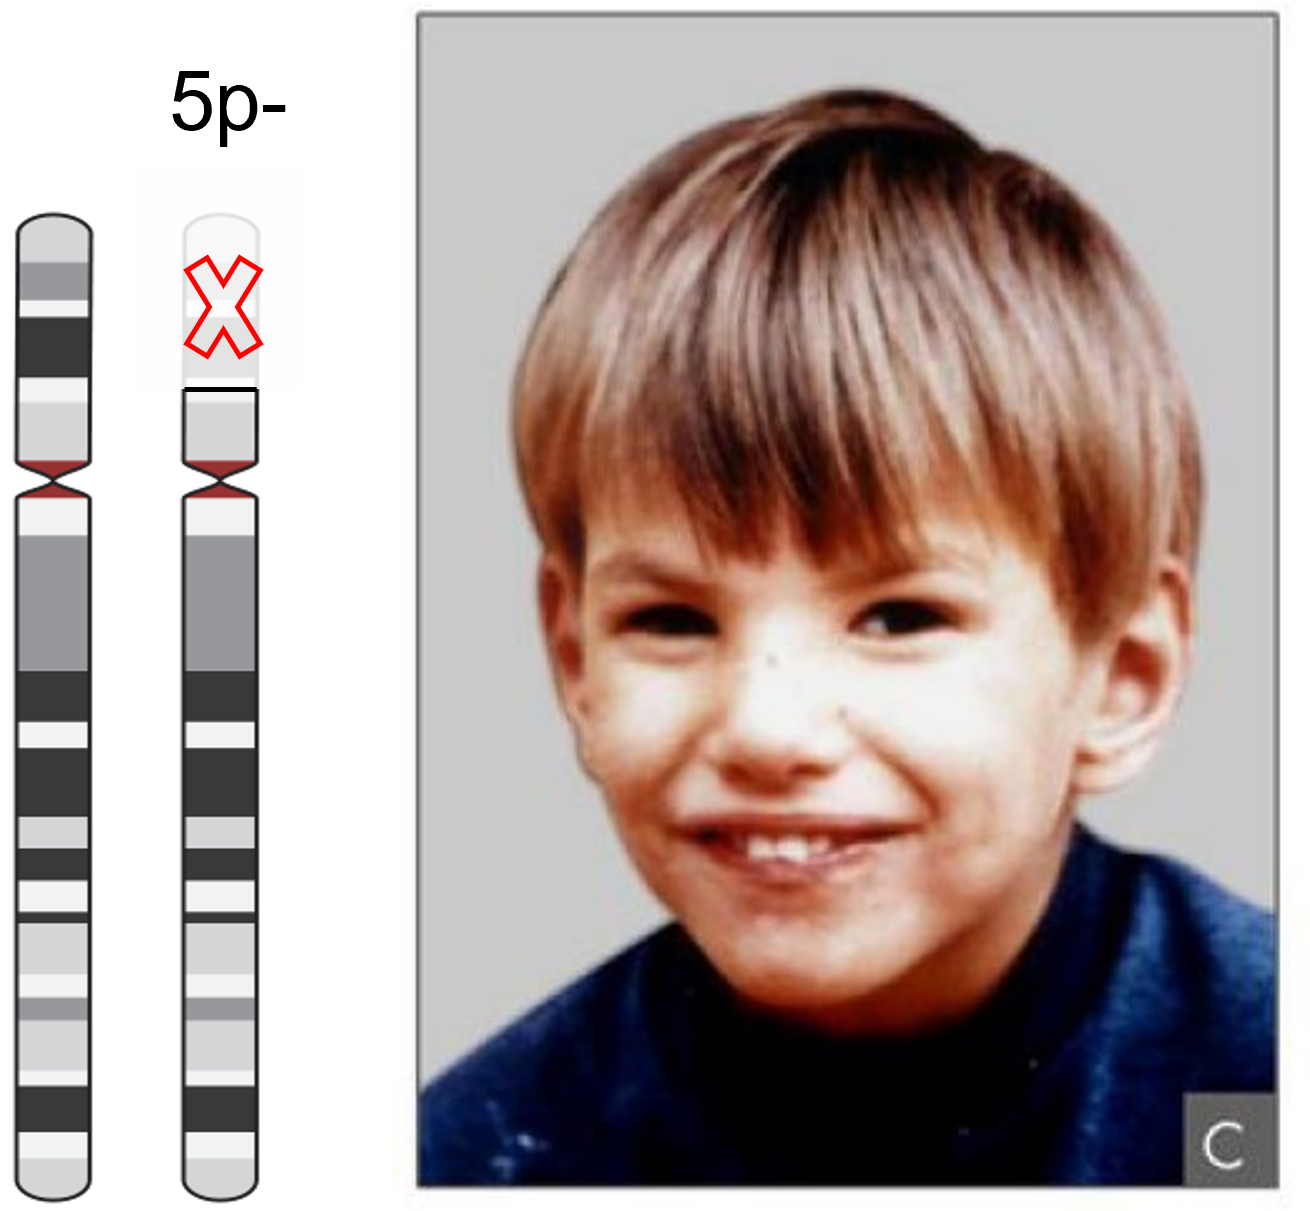
\includegraphics[width=0.25\linewidth]{files/cri-du-chat-1af99d4f92ed2247ec43b5a065c6d72d.png}
\end{figure}

Cri du chat syndrome is a genetic disorder that is caused by the partial
deletion of the short arm of chromosome 5. Babies suffering from the
condition have a high pitched cry that sounds similar to a cat, which has
given the condition its name.

Furthermore, they suffer a.o. from delayed growth and poor reflexes.
Credits: Image modified from \href{https://creativecommons.org/licenses/by/2.0}{CC-BY 2.0} \cite{cri-du-chat} and \href{http://creativecommons.org/licenses/by/4.0/}{CC-BY SA 4.0} \cite{chrom5}.
\end{framed}


\bigskip
\centerline{\rule{13cm}{0.4pt}}
\bigskip

\subparagraph{Structural variation}

Structural variants are variations that are larger than approximately 1kb in
size, which can occur within and between chromosomes. Structural variants
have the potential to have major influence on phenotypes, such as disease,
but that is not necessarily the case. Structural variants do appear to play
a large role in the development of cancerous cells.


\bigskip
\centerline{\rule{13cm}{0.4pt}}
\bigskip

\subparagraph{Copy number variation}

Copy number variants (CNVs) are a special case of structural variants where
the number of times a gene occurs on the genome changes. In a diploid
organism, a deletion will leave only one copy, whereas a duplication can
result in three or more copies of the gene in an individual. Changing the
copy number can be part of normal variation in a population, e.g., genes
involved in immune response vary in copy number; but, more often than not,
copy number variation leads to severe phenotype changes, such as diseases in
humans.


\bigskip
\centerline{\rule{13cm}{0.4pt}}
\bigskip

\subparagraph{Detection of structural variants}

Accurately detecting structural variation in a genome is not easy.  The
challenge lies in detecting the edges of the variants (the so-called
breakpoints) and, in case of duplications/insertions/deletions, the
resulting copy number.  When a mapping-based approach is used (possible if
the reference genome is known) we can use read depth and paired end reads to
detect variants.  More copies of the gene in the sample will result in more
reads from that gene (Figure~\ref{gene_duplication}) than expected for a single
copy.  Conversely, coverage is expected to drop when one copy of a gene is
lost.

\begin{figure}[!htbp]
\centering
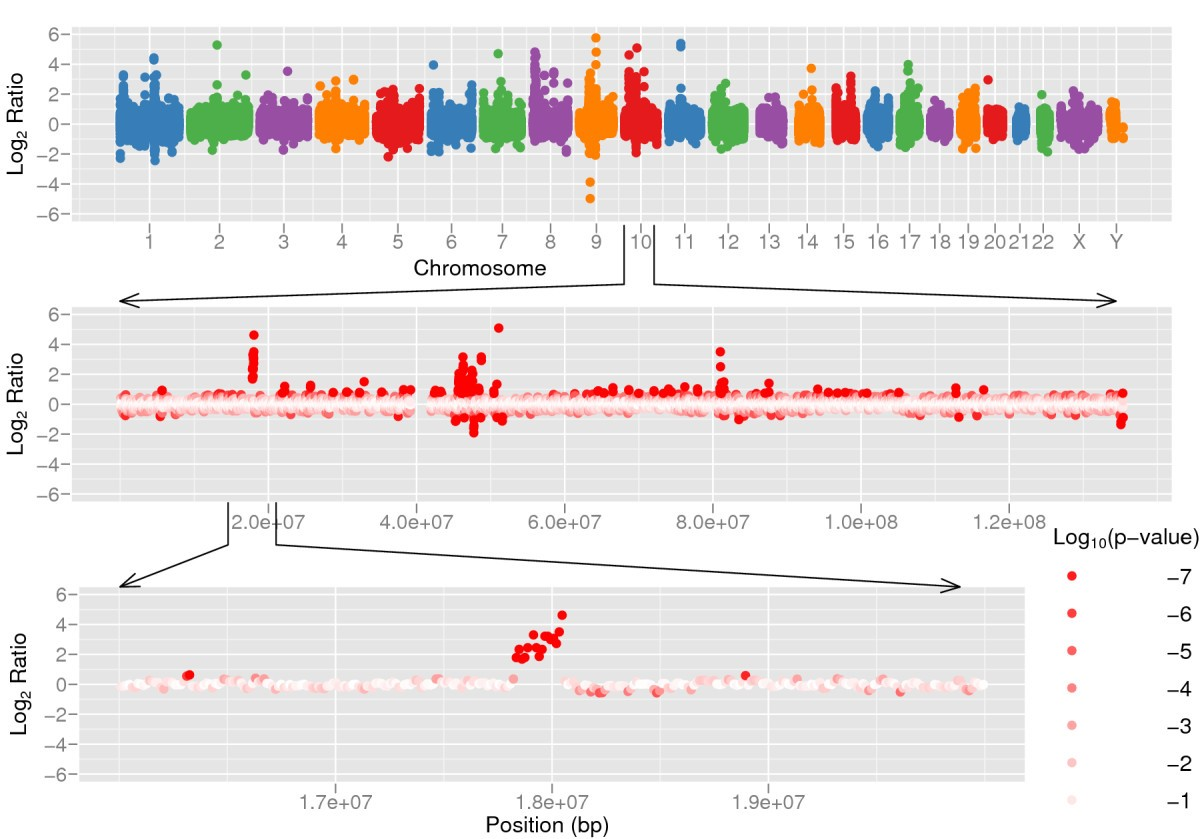
\includegraphics[width=0.7\linewidth]{files/gene-duplication-b8c950bcf6ab0c3a5d6ca3df673d2cba.jpg}
\caption[]{Gene duplication results in higher coverage than expected in the duplicated regions.
Credits: \href{https://creativecommons.org/licenses/by/2.0/}{CC BY 2.0} \cite{gene_duplication_2009}.}
\label{gene_duplication}
\end{figure}

Orientations of paired end reads as well as split reads are good
indicators to detect the boundaries of inversions, but also substitutions
and translocations. The rearrangements will result in one read from a pair
mapping to one genomic location and the other read to another location.
Reads overlapping the breakpoint will be split in the alignment.


\bigskip
\centerline{\rule{13cm}{0.4pt}}
\bigskip

\subparagraph{Examples of structural variants and CNVs}

\begin{figure}[!htbp]
\centering
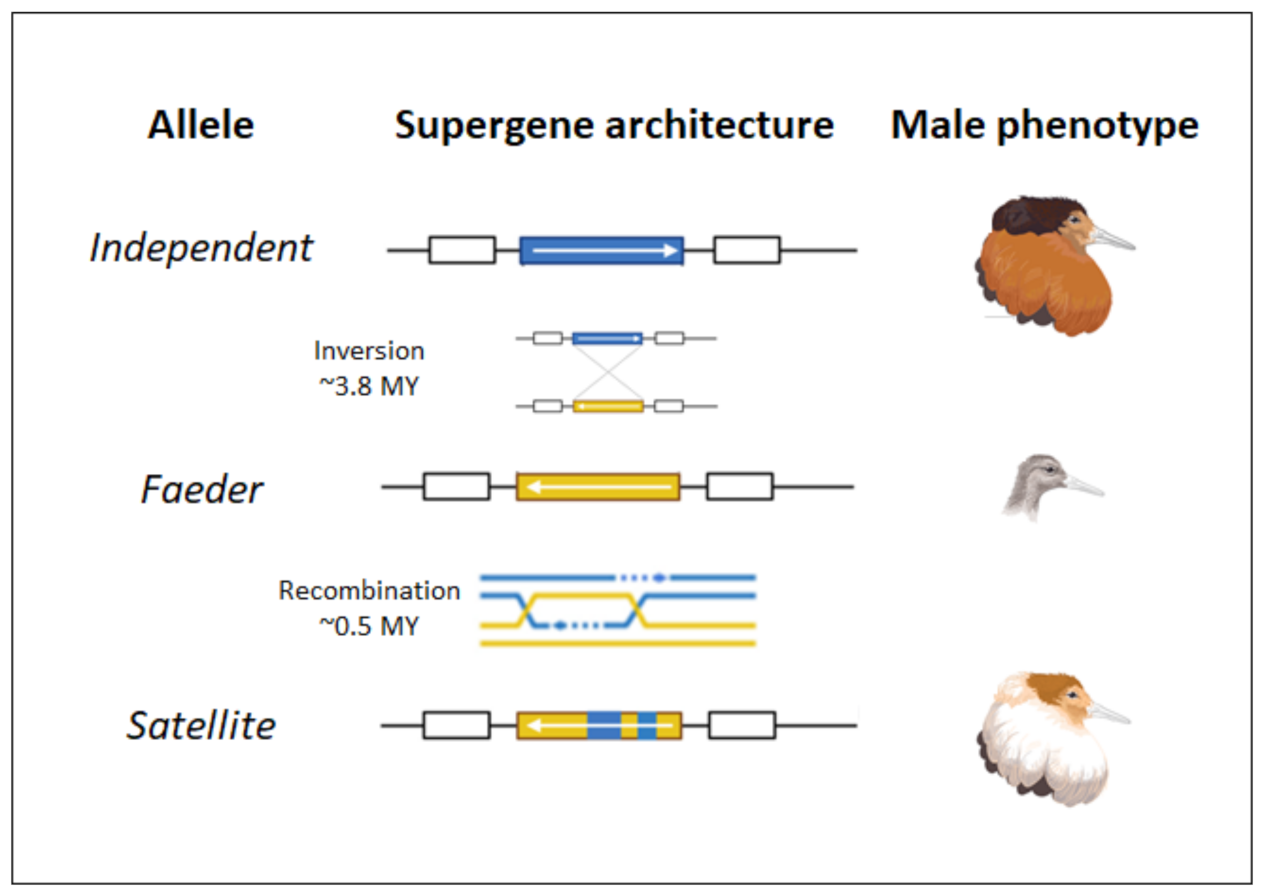
\includegraphics[width=0.7\linewidth]{files/male-morphs-c29897c340640f26b0227149c9ad8e0c.png}
\caption[]{Orientation of the inversion in the three male morphs.
Credits: \href{https://creativecommons.org/licenses/by/4.0/}{CC BY 4.0} \cite{male_morphs_2022}.}
\label{male_morphs}
\end{figure}

Large chromosomal inversions play a role in within-species phenotypic
variation and have also been found as the result of introgression after
hybridisation of two different species. One example of a within-species
inversion yielding large phenotypic differences are the three male morphs in
the ruff (\textit{Calidris pugnax}, Figure~\ref{male_morphs}).

\begin{figure}[!htbp]
\centering
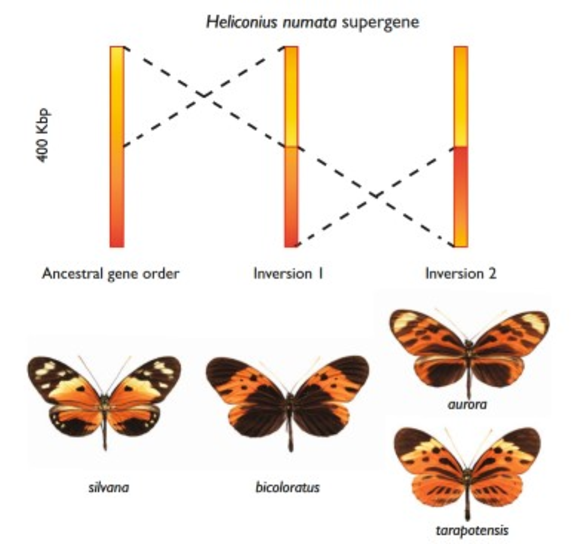
\includegraphics[width=0.7\linewidth]{files/butterflies-fbc698aca8b71a3df293b54d42f2b5fb.pdf}
\caption[]{At least two genetic inversions are associated with the \textit{Heliconius numata}
supergene. The ancestral gene order, which matches that in \textit{H. melpomene}
and \textit{H. erato}, is shown on the left and is associated with ancestral
phenotypes such as those found in \textit{H. n. silvana}. Two sequentially derived inversions
are associated with dominant alleles and are shown in the middle and right.
Credits: \href{https://creativecommons.org/licenses/by/4.0/}{CC BY 4.0} \cite{butterflies_2017}.}
\label{butterflies}
\end{figure}

Another example is the acquisition of an inversion containing genes for wing
color patterns in different species of Heliconius butterflies
(Figure~\ref{butterflies}). Copy number variation can also affect phenotypic traits
with an example being flowering time, photoperiod sensitivity, and height of
wheat plants (Figure~\ref{CNV}).

\begin{figure}[!htbp]
\centering
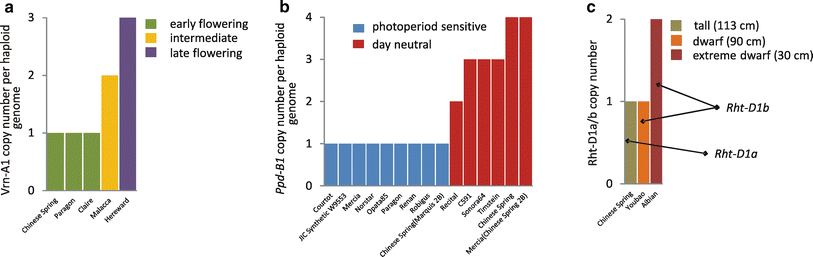
\includegraphics[width=0.7\linewidth]{files/CNV-55fecb2883a9e4c8ddc2f47636dbd31d.png}
\caption[]{Gene CNV contributes to wheat phenotypic diversity. a) CNV of \textit{Vrn-A1} gene
controls flowering time by affecting vernalization requirement; b) CNV of
\textit{Ppd-B1} controls flowering time by affecting photoperiod sensitivity; c)
CNV of \textit{Rht-D1b} gene (a truncated version of \textit{Rht-D1a}) determines severity
of plant dwarfism phenotype. In all three cases, the impact of gene copy
number on observed phenotype has been verified experimentally. Source data:
a, b, Díaz et al. (2012); c, Li et al. (2012).
Credits: \href{https://creativecommons.org/licenses/by/4.0/}{CC BY 4.0} \cite{CNV_2013}.}
\label{CNV}
\end{figure}


\bigskip
\centerline{\rule{13cm}{0.4pt}}
\bigskip

\subsubsection{Functional genomics and systems biology}

\begin{figure}[!htbp]
\centering
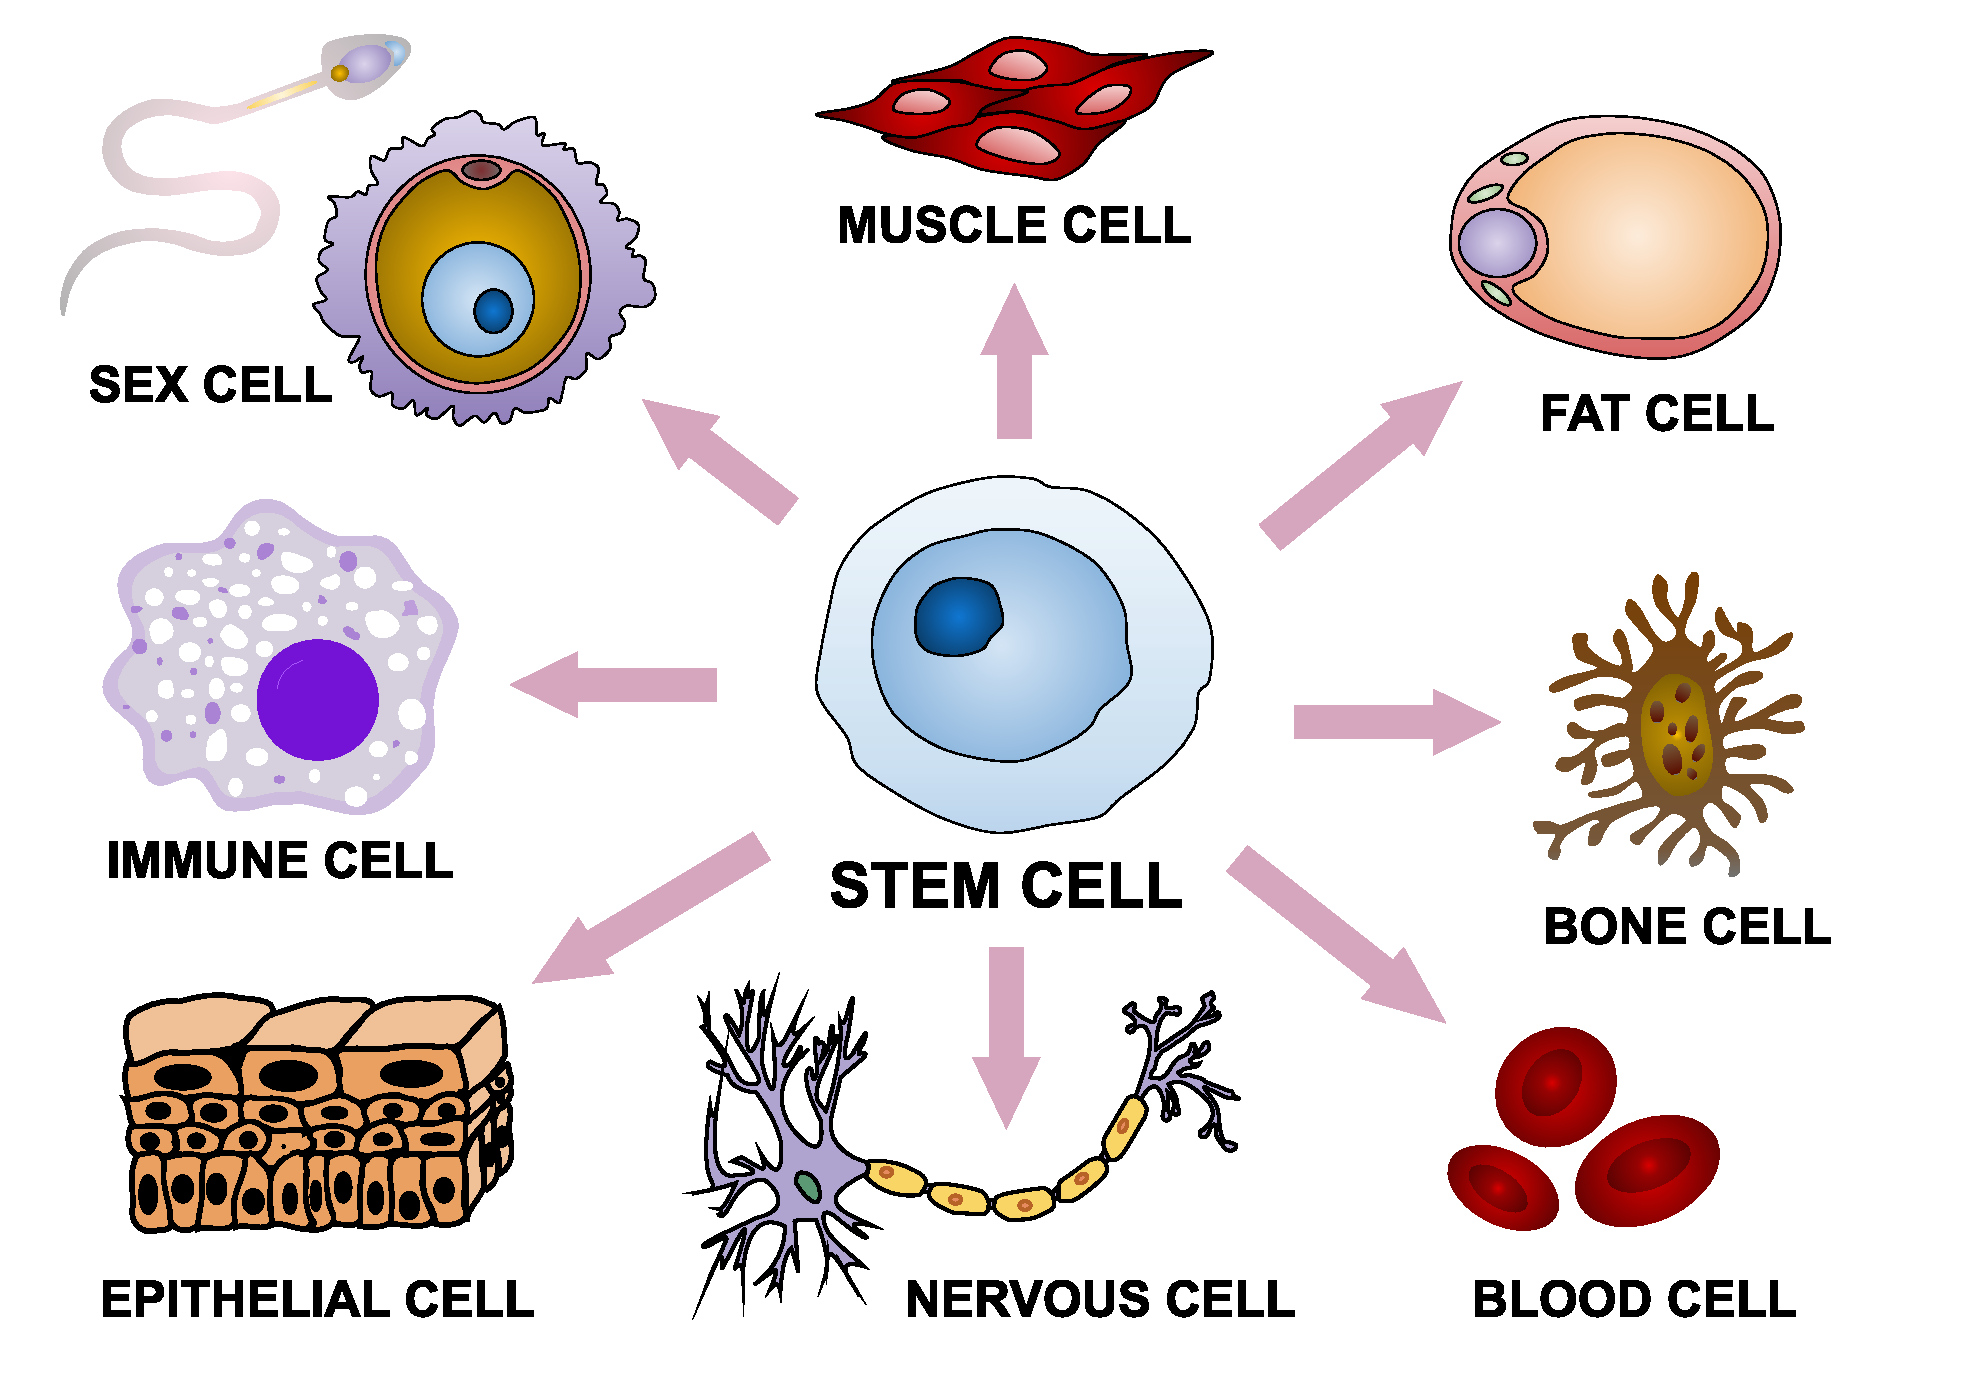
\includegraphics[width=0.5\linewidth]{files/stem-cell-241e430c225d6fa9f8242fe3f3222df6.pdf}
\caption[]{With the same genome, human stem cells differentiate into a wide range of shapes.
Credits: \href{https://creativecommons.org/licenses/by-sa/4.0/}{CC BY-SA 4.0} \cite{stem_cell_2019}.}
\label{stem_cell}
\end{figure}

\paragraph{The need for functional genomics}

While genomics provides us with an enormous amount of data on genomes and
genes, it is clear that these are only part of the story. Cells are not
static objects: they display different behaviour during their lifetime, and
react to changes in the environment and to signals from other cells. In
most multicellular organisms, cells in different organs develop in very
different ways, leading to different cell shapes, tissue organization and
behaviour (Figure~\ref{stem_cell}). Still, each cell contains the same genome, so there must be
differences in the way which that genome is used. In other words, if the genome is
the book of life, it must also contain the information on how to read it.

\begin{framed}
\textbf{Box 5.9: Epigenetics}\\
\begin{figure}[!htbp]
\centering
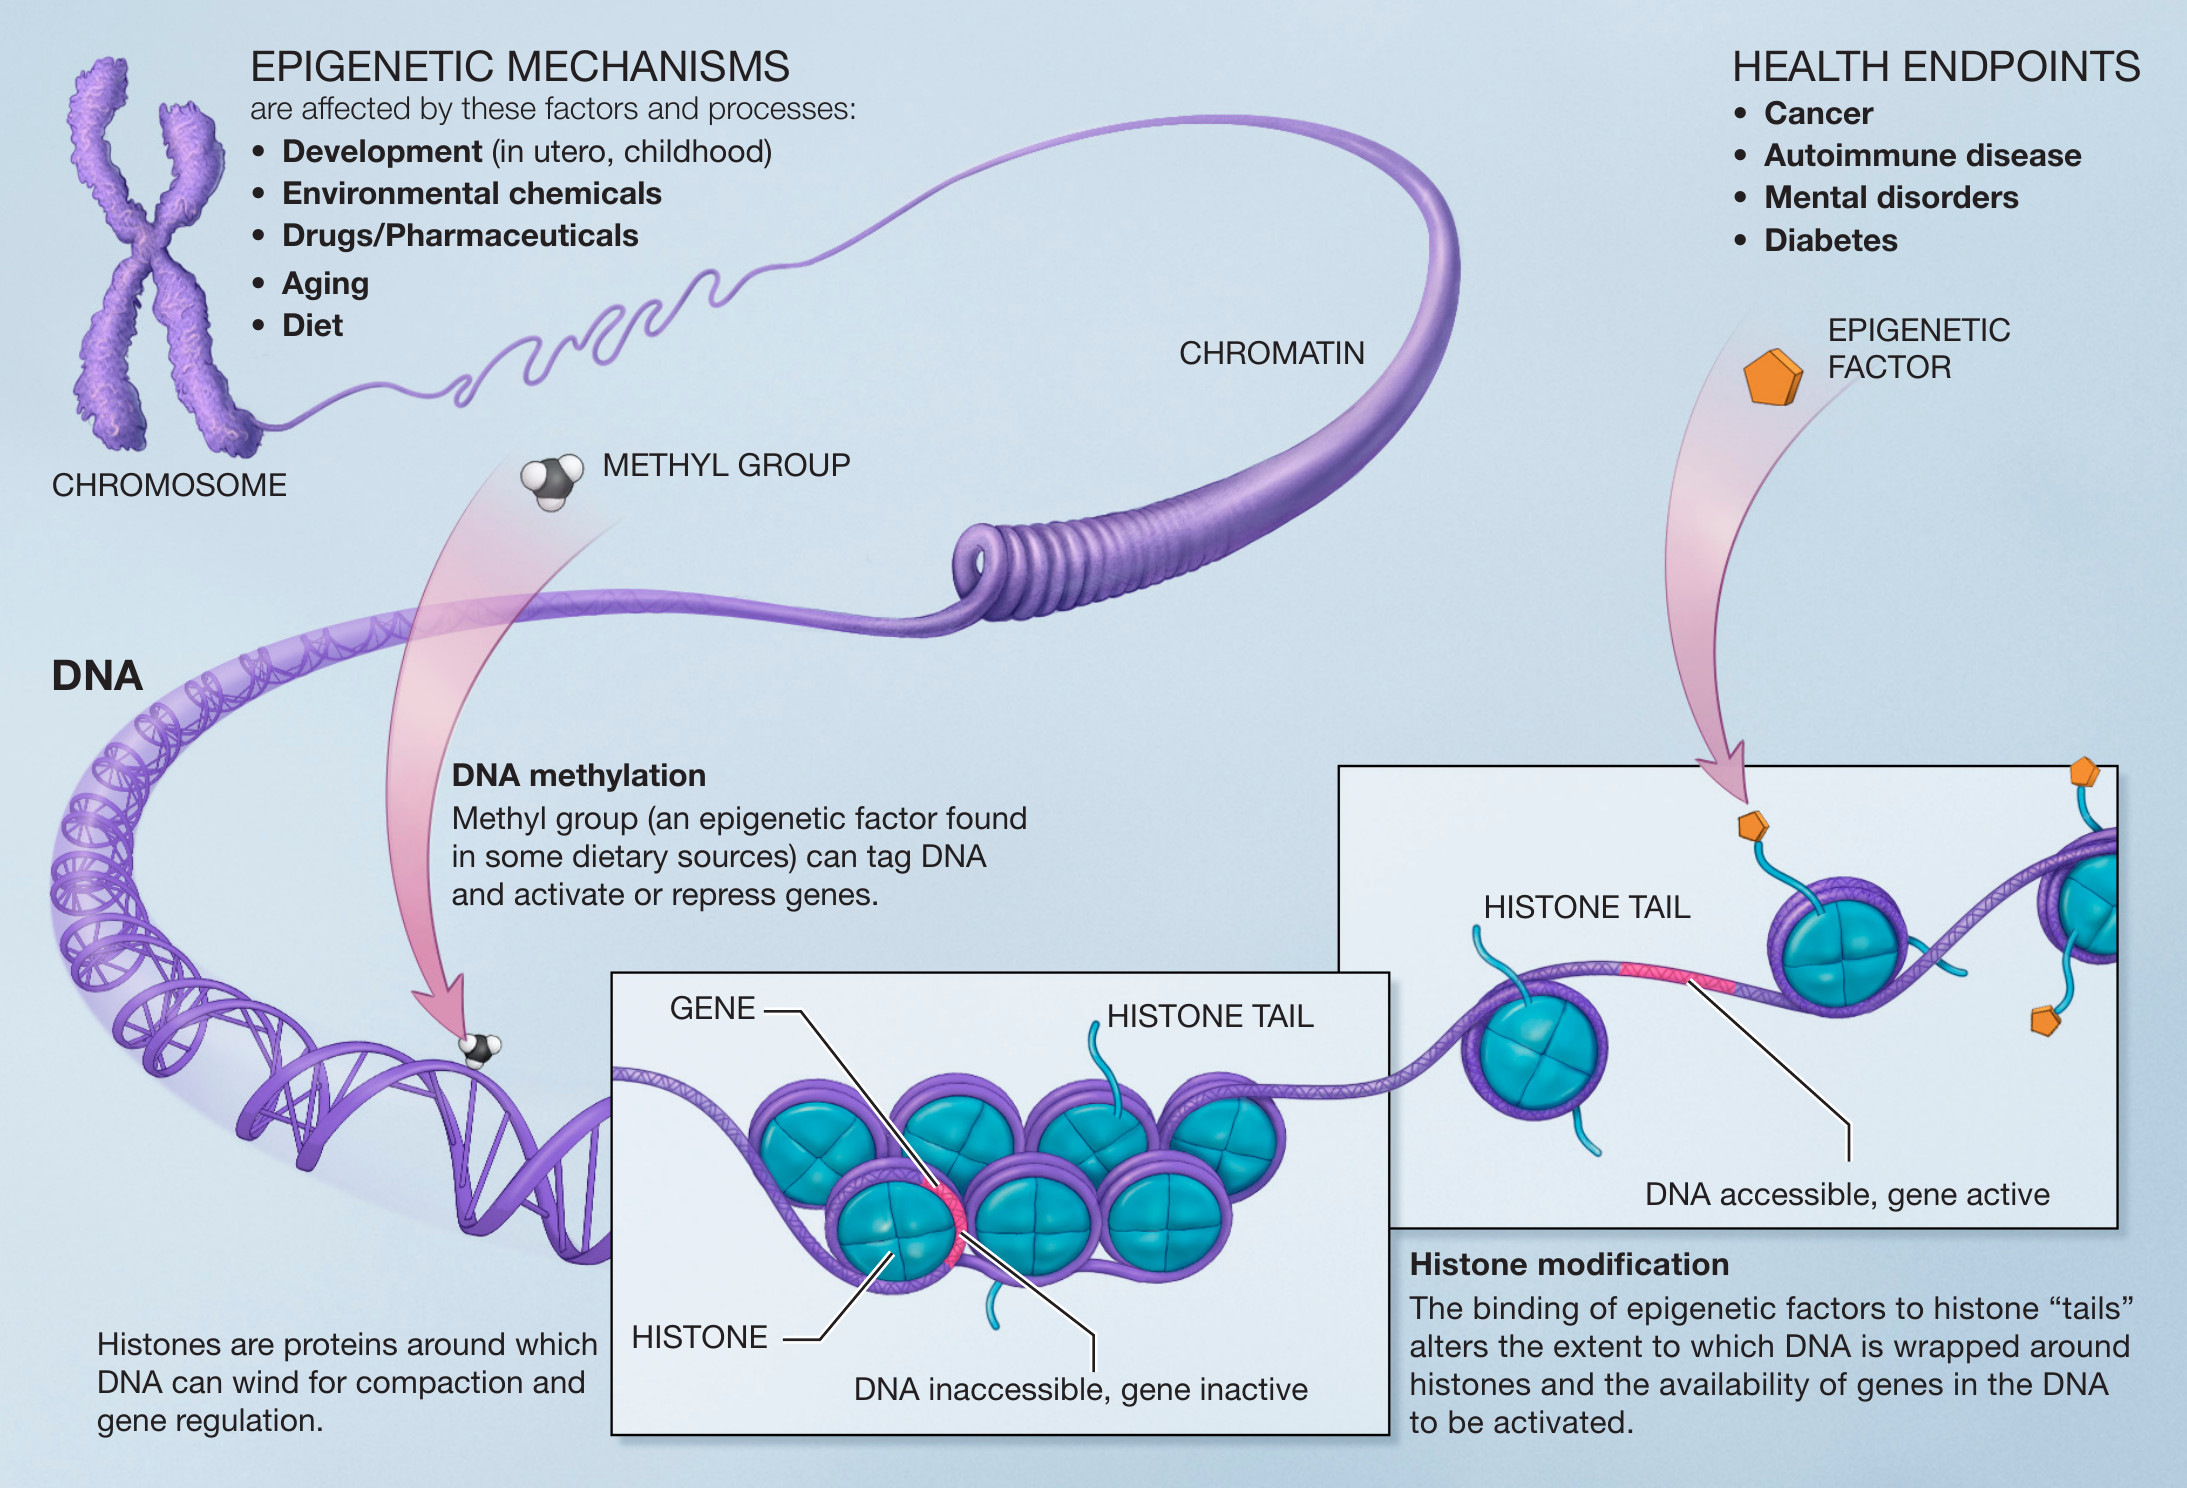
\includegraphics[width=1\linewidth]{files/epigenetics-30bb0bad64f2ca2bdc32b0b29f7ce6a8.png}
\caption[]{Epigenetic mechanisms are affected by several factors and processes
including development, environmental chemicals, drugs and pharmaceuticals,
aging, and nutrition. DNA methylation is what occurs when methyl groups, an
epigenetic factor found in some dietary sources, can tag DNA and activate or
repress genes. Histones are proteins around which DNA can wind for
compaction and gene regulation. Histone modification occurs when the
binding of epigenetic factors to histone ``tails'' alters the extent to which
DNA is wrapped around histones and the availability of genes in the DNA to
be activated. At a coarser level, the 3D organization of the DNA (``chromatin
structure'') also influences which regions of the genome are accessible for
transcription. In humans, all of these factors and processes can have an effect on
health and disruption can result in cancer,
autoimmune disease, mental disorders or diabetes, among other illnesses.
Credits: \href{https://creativecommons.org/publicdomain/zero/1.0/}{CC0 1.0} \cite{epigenetics_2005}.}
\label{epigenetics}
\end{figure}
\end{framed}

% #% The original URL in box 5.5 that is credited as the source leads to page that does not exist anymore. Changed to WikiMedia url. - The description is a literal copy paste from the figure description on WikiMedia.

A part of the explanation lies in what is called \textit{epigenetics},
modifications of the genome that do not change the DNA sequence but do
influence gene expression (Box~5.9). There are other mechanisms besides
epigenetics that control how genes are expressed, and how the resulting
proteins eventually fulfil their function in the cell. The most well-known
ones are interactions between proteins and DNA (transcription factors and
enhancers, influencing expression); interactions between proteins, to form
complexes or to pass signals; and catalysis of metabolic reactions by
enzymes.

The field of research that studies how genes are used is called \textit{functional
genomics}. The most prominent functional genomics project started
immediately following the completion of the human genome: the ENCODE
(``Encyclopedia of DNA elements'') project (2005-2015), aiming to identify all
functional parts of the genome.


\bigskip
\centerline{\rule{13cm}{0.4pt}}
\bigskip

\subparagraph{The role of omics data}

Functional genomics research mostly measures cellular activities in terms of
the abundance of genes, proteins and metabolites, and the interaction
between these molecules. When performed at a cell-wide level, i.e.,
attempting to measure all molecules of a certain type at once, these are
called \textit{omics} measurements. The technology to measure such omics data is
usually \textit{high-throughput}, which means that little manual work or repetition
of experiments are needed. We generally distinguish five main levels of omics
measurements as illustrated in Figure~\ref{omics_levels}, although many new omics terms are
still being introduced. Next to genomics, the following omics measure:

\begin{itemize}
\item Epigenomics: all epigenetic modifications of the genome.
\item Transcriptomics: the expression levels of all genes.
\item Proteomics: the presence/quantity of all proteins.
\item Metabolomics: the presence/quantity of all metabolites.
\item Phenomics: the eventual phenotype(s), i.e., form or behaviour, of a cell or organism.
\end{itemize}

Such measurements are increasingly also applied on mixed samples, mostly
bacterial/fungal/viral communities such as found in the human gut and in the soil.
As a kind of `meta' analysis, this has been labelled metagenomics,
metatranscriptomics, etc.

The introduction of omics technologies over the last 25 years has broadened
the field of bioinformatics and made it increasingly relevant to all areas
of biology. Very large measurement datasets are now routinely produced and
should be cleaned, checked for quality and processed.
Moreover, the data should be stored in databases to make it accessible and
re-usable for further research. Finally, careful analysis, interpretation and
visualization of the data is essential to allow biologists to infer
biological functions. Bioinformatics delivers the tools and databases to
support all these steps.

Even though omics measurements provide highly detailed overviews of
cellular states and reactions to perturbations, there are a number of
important limitations:

\begin{itemize}
\item Experimental cost: omics devices are often expensive to acquire, and each
experiment requires labour and consumables
\item Technical noise: all measurements technologies come with inherent variation and
measurement noise
\item Biological variation: different cells, organs or individuals will differ
in their biological state and make-up
\item Bias and coverage: most omics technologies are most efficient (or even
only work) for measuring specific types of molecules or interactions
\end{itemize}

% #%	Moreover, omics measurements are often indirect, measuring the effects of certain molecules or interactions through other readouts (for example, by imaging fluorescent markers, or by translating RNA to DNA for subsequent sequencing) or measuring only parts of molecules. Such technologies require steps in data analysis to translate the measurements back to what we actually wanted to measure, which also introduces noise.
% #% when studying the effect of a mutation or intervention by comparing two samples, ideally all other biological circumstances should be identical. In practice, cells are dynamic (e.g., cell cycle) and sensitive to environmental influence. Similarly, molecule levels and interactions are dynamic: molecules are produced, transported, modified, and degraded continuously, and a measurement at a specific time point is only a snapshot.
% #%, or work best for certain ranges of levels. It is often also hard to take the many different functional forms of a molecule, such as modified proteins, into account. Some technologies are even limited to measuring a subset of all possible molecules or interactions. This means that care must be taken when analyzing the resulting data; in particular, _not_ measuring something does not mean it is not there.

Typically, functional genomics experiments involve studying the effect of
genetic variation on certain omics levels.  Such variation can be natural,
for example comparing omics data measured on two organisms with known
(limited) genetic differences due to evolution.  It can also be
experimentally introduced, for example by introducing small mutations in the
DNA sequence, knocking out genes, introducing new genes etc.  Variation can
also be introduced in the environment, e.g. by changing the
temperature, adding or removing nutrients, introducing drugs etc. The effects of
such interventions at a specific omics level then provide information on the
function of the manipulated gene(s) or the effect of the environment.

% @% Ideally we would measure different omics levels at the same time (multi-omics) and even in the same sample (paired omics), but this is often experimentally too complex and costly. Some omics technologies are more acccessible than others, in terms of cost, data quality, and interpretation and are therefore most widely used - in particular, gene expression levels (transcriptomics) are often measured and assumed to reflect the overall state of a cell. However, as discussed [below](chapter5_omics), we should be careful with this.

\subparagraph{From functional genomics to systems biology}

Where functional genomics uses omics measurements to learn about the role
of genes and proteins in the cell, individual experiments and measurements
generally only provide individual pieces of the puzzle, which often do not
make much sense without understanding other cellular processes. Recognizing
the need for a more holistic approach, systems biology was proposed as a
scientific approach in which the main goal is to construct models of living
systems, that are increasingly refined by hypothesis formation,
experimentation, and model extension or modification.

\begin{figure}[!htbp]
\centering
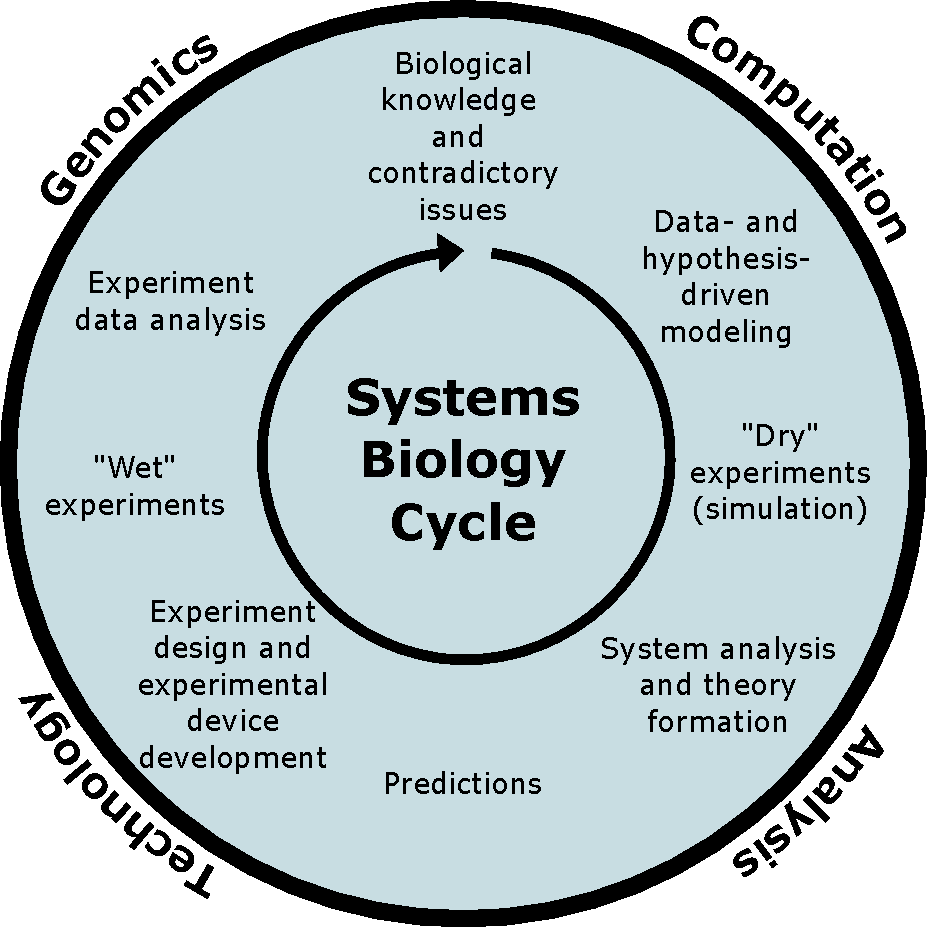
\includegraphics[width=0.5\linewidth]{files/systems-biology_alt-1ec51eb64581d8097f689b71d4f29d6e.pdf}
\caption[]{The systems biology cycle, aiming to iteratively improve models of living systems
(based on \cite{systems_biology_2002}).
Credits: \href{https://creativecommons.org/licenses/by/4.0/}{CC BY-NC 4.0} \cite{own_5_2024}.}
\label{systems_biology_alt}
\end{figure}

Eventually, the hope of systems biology is to arrive at systems-level
understanding of life that will allow us to simulate the effects of
interventions (mutations, drug treatments, etc.) or even (re)design genes and
proteins to improve certain behaviour, such as production levels of desired
compounds in biotechnology. While we still have a long way to go, omics
data analysis is an essential element in systems biology.


\bigskip
\centerline{\rule{13cm}{0.4pt}}
\bigskip

\paragraph{Transcriptomics}\label{chapter5_transcriptomics}

Transcriptomics is concerned with measuring the expression of genes (i.e.,
the levels of transcription of genes on the genome to RNA). RNA and its
role in the cell has already been discussed in chapter~1. If you want to know
what other types of RNA exist outside the common mRNA, miRNA, tRNA and rRNA, read
Box~5.10. Here we focus on measuring and counting transcripts (mRNA).

% #% Chapter 1 does also mention miRNA as one of the main types of RNA.

For the understanding of transcriptome analysis it is important to remember
that in eukaryotes most genes contain introns and that one gene can have
many transcripts.

\begin{framed}
\textbf{Box 5.10: The RNA world}\\
Many other types of RNA exist in the cell and they perform important regulatory functions:

\begin{itemize}
\item miRNA (micro RNA): small (20-21nt) pieces of RNA that are cut from a longer pre-miRNA hairpin.
miRNAs bind to target sites in mRNA and prevent binding of the messenger.
\item siRNA (short interfering RNA): are generally 20-24nt long pieces of RNA that work similar to miRNAs but instead of actively preventing translation, the targeted mRNA is cut into pieces and destroyed.
\end{itemize}

\begin{figure}[!htbp]
\centering
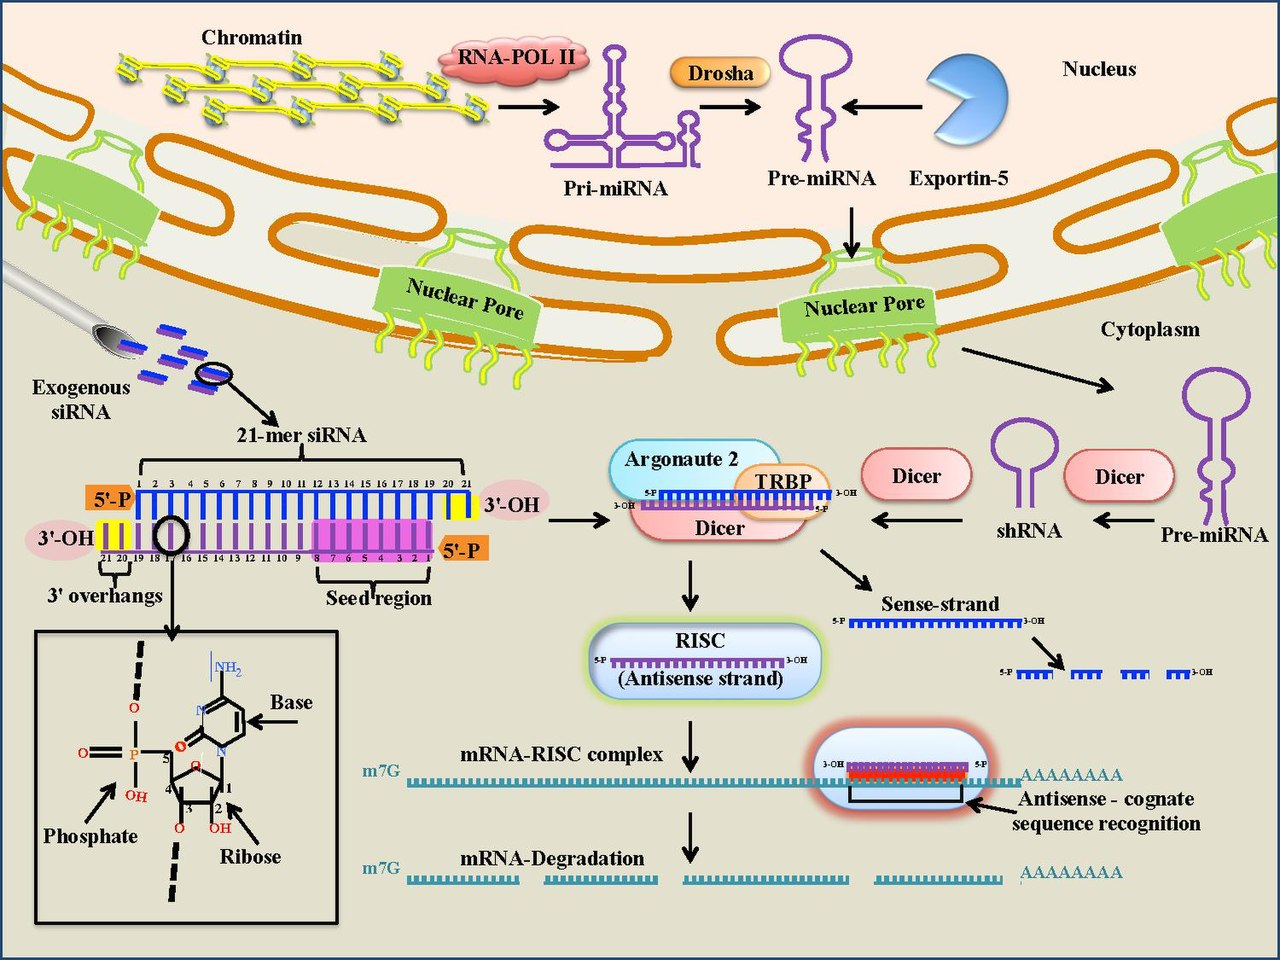
\includegraphics[width=1\linewidth]{files/RNA-types-a2df13784fce13387140a3a6c290b2ab.jpg}
\caption[]{The generalized RNAi mechanism up to the molecular level depicting the role of various cellular proteins and external siRNAs. Credits: \href{https://creativecommons.org/licenses/by-sa/4.0/}{CC BY-SA 4.0} modified from \cite{RNA_types_2016}.}
\label{RNA_types}
\end{figure}

\begin{itemize}
\item snoRNA (small nucleolar RNA): guides the methylation and pseudouridylation of ribosomal RNA required in the mature rRNA.
\item lncRNA (long non-coding RNA): \textgreater 200nt long stretches of RNA that arise from transcription but (appear to) have no open reading frame.
How many of these lncRNAs have a specific function and what that function might be is not clear. Most might simply be the result of pervasive transcription.
\item piRNA (piwi interacting RNA): found in animals and slightly longer than miRNAs (26-31nt), they interact with piwi proteins. piRNAs are implicated in epigenetic gene silencing, but not much is known.
\end{itemize}
\end{framed}

% #% Figure RNA_types is rather blurry and unclear. Replace image that better depicts the different types of RNA?

In transcriptomics, the aim is to measure presence and abundance of
transcripts. Such measurements are based on a large number of cells, but
more recently the transcriptome of individual cells can also be studied. So
what do transcripts and their abundance tell us about a studied subject? In
any experiment we often want to know what happens to a cell/tissue/organism
under certain circumstances. Most informative for this are protein levels
and even more specifically protein activity, as these directly influence what
happens. As will be discussed below, detecting and measuring proteins is
complex. Measuring mRNA levels is far easier, but it is important to
realise that they only provide a proxy to what happens in a cell. mRNA
levels do not always correlate with protein levels as transcripts can be
regulated or inhibited, affecting translation. Protein levels can be
equally affected by regulation and abundance does not always correlate with
activity.

Despite its limitations, we can address a number of very relevant questions
based on transcriptomics measurements. Three general analyses will be
discussed below, but note that to detect relationships between experimental
conditions and mRNA expression patterns, it is important to be aware what
can cause variation in mRNA levels. Some of these causes may be intended
variation, some will cause noise.

mRNA levels:

\begin{itemize}
\item are the result of mRNA synthesis and mRNA decay
\item differ between genes, isoforms, cells, cell types and tissues, and developmental stages
\item vary with cell cycle, during the day (circadian rhythm) and/or season
\item depend on the environment
\end{itemize}


\bigskip
\centerline{\rule{13cm}{0.4pt}}
\bigskip

\subparagraph{How to measure mRNAs?}

Just like the study of genomes, transcriptomics has greatly benefitted from
technological developments that allowed an increase in throughput and
sensitivity of measurements.  Box~5.11 and
Box~5.12 provide an overview of technologies that were
important for the development of the field (such as microarrays), but are
not widely used anymore; at this time, RNAseq is almost exclusively used to
measure mRNA levels.

Note that microarrays haves now been mostly superseded by RNAseq as a
cheaper and better quality alternative (see below).
However, there are many microarray samples still available for re-use in
databases, as submission of measurement data to such databases is compulsory
upon publication of a scientific paper.  The most well-known repositories
are the NCBI Gene Expression Omnibus
(\href{https://www.ncbi.nlm.nih.gov/geo/}{GEO}), with as of March 2024 {\textasciitilde}7.1
million samples, and \href{https://www.ebi.ac.uk/biostudies/arrayexpress}{EBI
ArrayExpress}.  If you are
interested in a certain question that may be answered using transcriptomics,
it makes sense to look here first to see what experimental data is already
available. Note that the technology used determines how the expression
level should be interpreted (see box below).

\begin{framed}
\textbf{Important to know about microarrays}\\
\begin{itemize}
\item microarrays measure expression indirectly, using fluorescence; as a
result, measurements can be noisy and have a low dynamic range (i.e., low
expression levels cannot be measured well)
\item some microarray types compare two samples and thus produce relative expression levels, often log\textsubscript{2}-transformed so that 0 means no change, +1
means a 2-fold higher expression, +2 a 4-fold higher expression and so on; negative numbers indicate lower expression
\item other microarray types measure levels that represent absolute expression in a single sample (in arbitrary
units); normalization is then important when comparing measurements between samples
\end{itemize}
\end{framed}

\begin{framed}
\textbf{Box 5.11: Gels and qPCR}\\
\begin{figure}[!htbp]
\centering
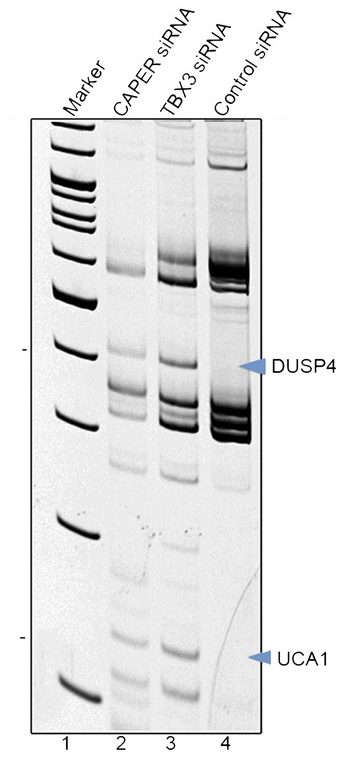
\includegraphics[width=0.23\linewidth]{files/differential-gel_alt-71930b59285dc178cf571ccbfbb991dd.png}
\caption[]{Example of differential \newline
display gel. Credits: \href{https://creativecommons.org/licenses/by/3.0/}{CC BY 3.0} \newline
modified from \newline
\cite{differential_gel_alt_2014}.}
\label{differential_gel_alt}
\end{figure}

Early methods of detecting transcripts and expression levels are northern
blots and differential display (Figure~\ref{differential_gel_alt}).  Both are
gel-based methods, low throughput and not very accurate.  Northern blots and
differential displays were superseded by qPCR (quantitative PCR) and
microarrays (see Box~5.7).  Quantitative real-time PCR
(qPCR) is a PCR (polymerase chain reaction) that measures the abundance of
each DNA molecule by adding a fluorescent reporter, either a dye that binds
DNA or fluorescent probes.  The level of fluorescence increases with the
number of amplified fragments, which in turn is detected.  When the reaction
passes a threshold at a given cycle, the cycle number is used to deduce the
original amount of template fragments in the reaction (Figure~\ref{qPCR_alt}).
qPCR is often used to validate results obtained by other quantitative
methods.

\begin{figure}[!htbp]
\centering
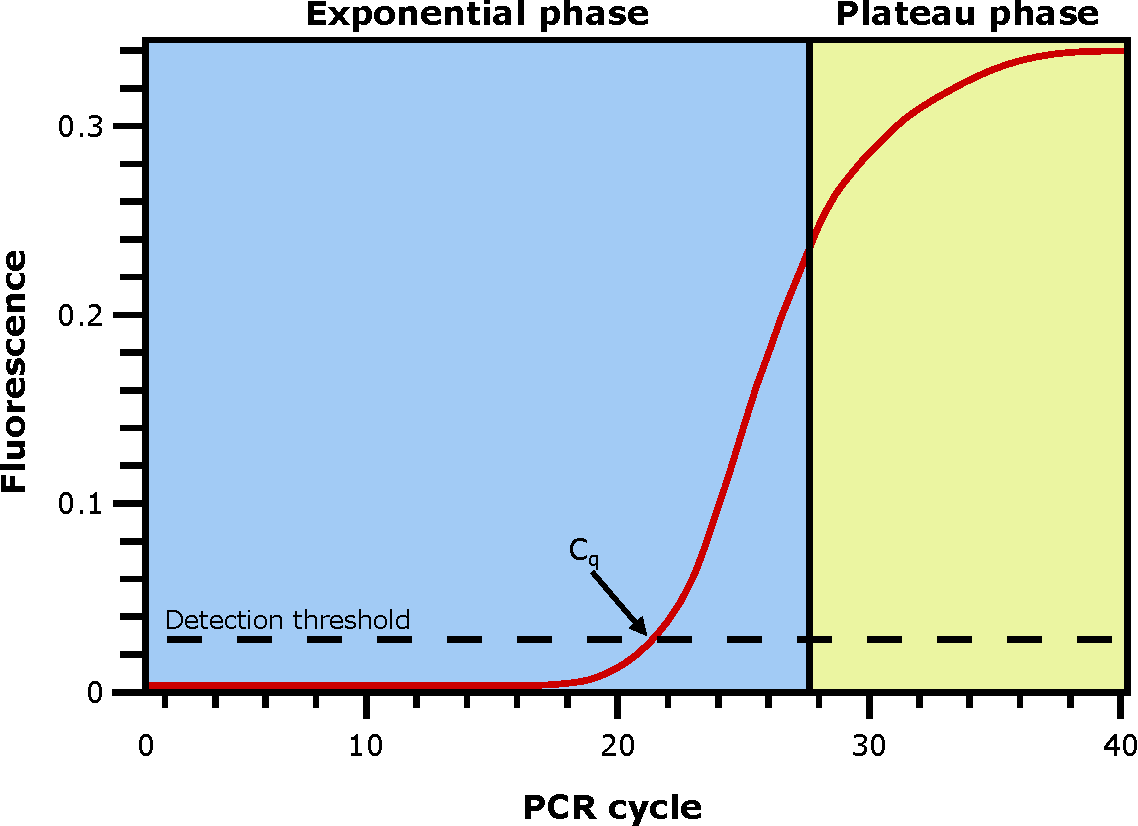
\includegraphics[width=0.8\linewidth]{files/qPCR_alt-0dda6e612266ad607e736b1a883a2b76.pdf}
\caption[]{Amplification plot of a DNA fragment in a qPCR reaction.
C\textsubscript{q} corresponds to the cycle were fluorescence passes the detection threshold.
Credits: \href{https://creativecommons.org/licenses/by-nc/4.0/}{CC BY-NC 4.0} \cite{own_5_2024}.}
\label{qPCR_alt}
\end{figure}
\end{framed}


\bigskip
\centerline{\rule{13cm}{0.4pt}}
\bigskip

\subparagraph{Microarrays}\label{chapter5_microarrays}

\begin{framed}
\textbf{Box 5.12: Microarrays}\\
The first widely used \textit{high-throughput} method to measure gene expression
was the microarray. DNA microarrays are based on the principle that
complementary strands of DNA bind each other. Microarrays are
typically flat surfaces (slides of glass or some other material) with
microscopic spots of single-strand DNA sequences - so-called probes -
at known locations, ranging from a few thousand to millions. Each
DNA sequence is chosen to (as best as possible) represent a specific gene,
i.e., a unique subsequence. This means that microarrays can only be
designed to detect known genes and are organism-specific, and that gene
variants (SNPs, splice variants) are hard to detect.

In microarray experiments, mRNA molecules are first selected by looking for
a poly-A tail, converted into complementary DNA (cDNA), labelled with a
fluorescent dye and washed over the surface.  Complementary sequences will
bind, and after some time the unbound material is washed off and
fluorescence is measured using a microscope.  The light intensity level at a
certain location on the surface is then an indirect readout for the number
of sequences that bound, and thus for the relative expression of the
corresponding gene.


\bigskip
\centerline{\rule{13cm}{0.4pt}}
\bigskip

\begin{figure}[!htbp]
\centering
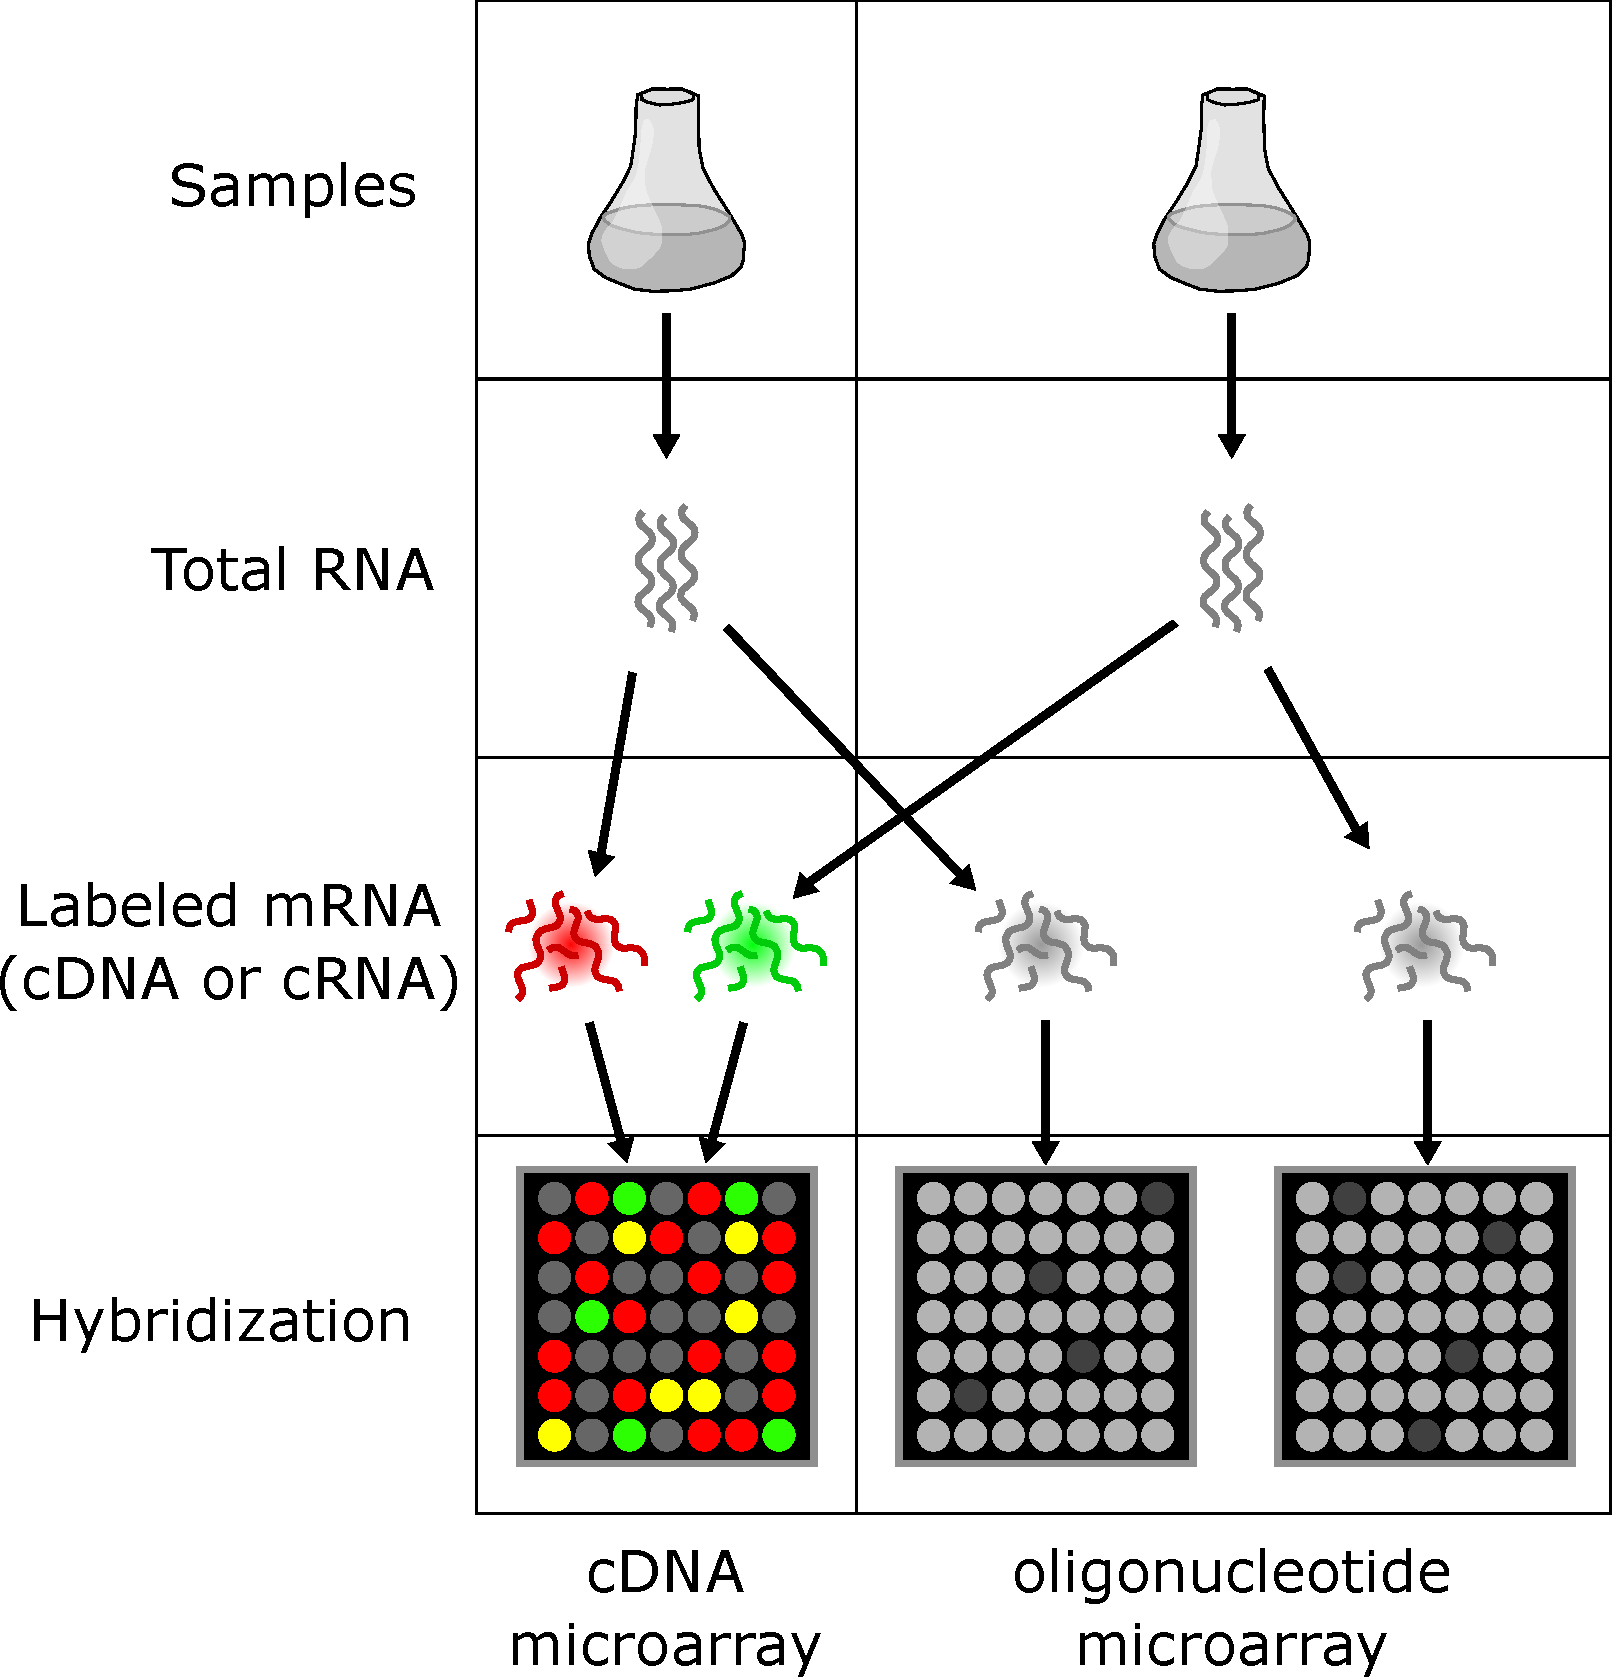
\includegraphics[width=0.7\linewidth]{files/microarrays_alt-f6a1faf71b62e633ac6d22495eae4072.pdf}
\caption[]{The difference between cDNA (two-color) and oligonucleotide (one-color) microarray analysis.
Credits: \href{https://creativecommons.org/licenses/by-nc/4.0/}{CC BY-NC 4.0} \cite{own_5_2024}.}
\label{microarrays_alt}
\end{figure}

There are two main competing types of microarrays: cDNA and oligonucleotide
arrays. While the principles are the same, they differ in production and
use (as illustrated in Figure~\ref{microarrays_alt}):

\begin{itemize}
\item \textbf{cDNA microarrays} contain long probes, of several hundreds of
nucleotides up to 1000nt. They can be produced in the lab by spotting
robots, and so easily be adjusted for specific experiments. This comes
with greater variation between microarrays, making it harder to compare
different measurements. cDNA microarrays are therefore mostly used for
direct comparisons between two samples, in which both samples (for example,
healthy and diseased tissue) are labelled with different fluorophores -
usually Cy3 (green) and Cy5 (red). The relative number of DNA sequences
bound then reflects the relative concentration of an mRNA molecule in sample
1 and sample 2, and thus the colour. A green spot means only sample 1
contained the corresponding mRNA molecule, a red spot means that it was
found in sample 2 and a yellow spot that it was found in both samples. The
intensity then reflects the overall expression level: black/dark for low
expression in both samples, bright for high expression.
\item \textbf{oligonucleotide microarrays} contain short probes (25nt), which are
produced using technology similar to microchip production. This means
quality is high and constant, and different arrays can easily be compared.
Oligonucleotide arrays therefore usually measure just a single sample using
one colour. However, as short probes are less likely to be unique for a gene,
transcripts are usually measured by combining multiple probes in so-called
probesets.
\end{itemize}

Overall, microarray measurements are often noisy and cannot distinguish very
low expression levels, as they do not provide enough fluorescence
signal. Data normalization is therefore also an important step, to remove
non-relevant variation between different microarray measurements.
\end{framed}


\bigskip
\centerline{\rule{13cm}{0.4pt}}
\bigskip

% ##### Repositories
% 
% While popular in the 1990s and early 2000s, microarrays haves now been
% mostly superseded by RNAseq as a cheaper and better quality alternative (see
% [below](chapter5_rnaseq)). However, there are many microarray samples still available for
% re-use in databases, as submission of measurement data to such databases is
% compulsory upon publication of a scientific paper. The most well-known
% repositories are the NCBI Gene Expression Omnibus ([GEO](https://www.ncbi.nlm.nih.gov/geo/)),
% with as of March 2024 ~7.1 million samples, and [EBI ArrayExpress](https://www.ebi.ac.uk/biostudies/arrayexpress).
% If you are interested in a certain question that may be answered using transcriptomics,
% it makes sense to look here first to see what experimental data is already available.


\bigskip
\centerline{\rule{13cm}{0.4pt}}
\bigskip

\subparagraph{RNAseq}\label{chapter5_rnaseq}

RNAseq makes use of affordable and reliable sequencing methods. Important
for the development of RNAseq was the reliable quantitative nature of NGS
protocols and sequencers. RNAseq is untargeted: all RNA in a sample can in
principle be sequenced and it is not necessary to have prior knowledge of
transcript sequences. While RNAseq is mainly used to study transcript
abundance, it can also be used to detect transcript isoforms (and their
abundance), as well as variants (see Variants above).

% :::{admonition} Box 5.11: Ever more detail
% :class: tip
% 
% Until now, most RNAseq experiments have been performed on groups of cells,
% as sequencing devices require large amounts of DNA. This means that cells
% of different cell types or different life stages are included in a single
% sample. While detection of differentially expressed genes is clearly
% possible with this method, weak or more nuanced variation is averaged out
% across all cells. Recently, methods have become available that separate
% tissues into individual cells and sequence each of these separately. This
% does require PCR amplification of RNA to reach the amounts required for
% sequencing, as well as sophisticated bioinformatics and statistical methods
% to deal with the resulting data. For a review, see this [paper](https://genomebiology.biomedcentral.com/articles/10.1186/s13059-016-0927-y).
% :::


\bigskip
\centerline{\rule{13cm}{0.4pt}}
\bigskip

\subparagraph{Protocol}

\begin{figure}[!htbp]
\centering
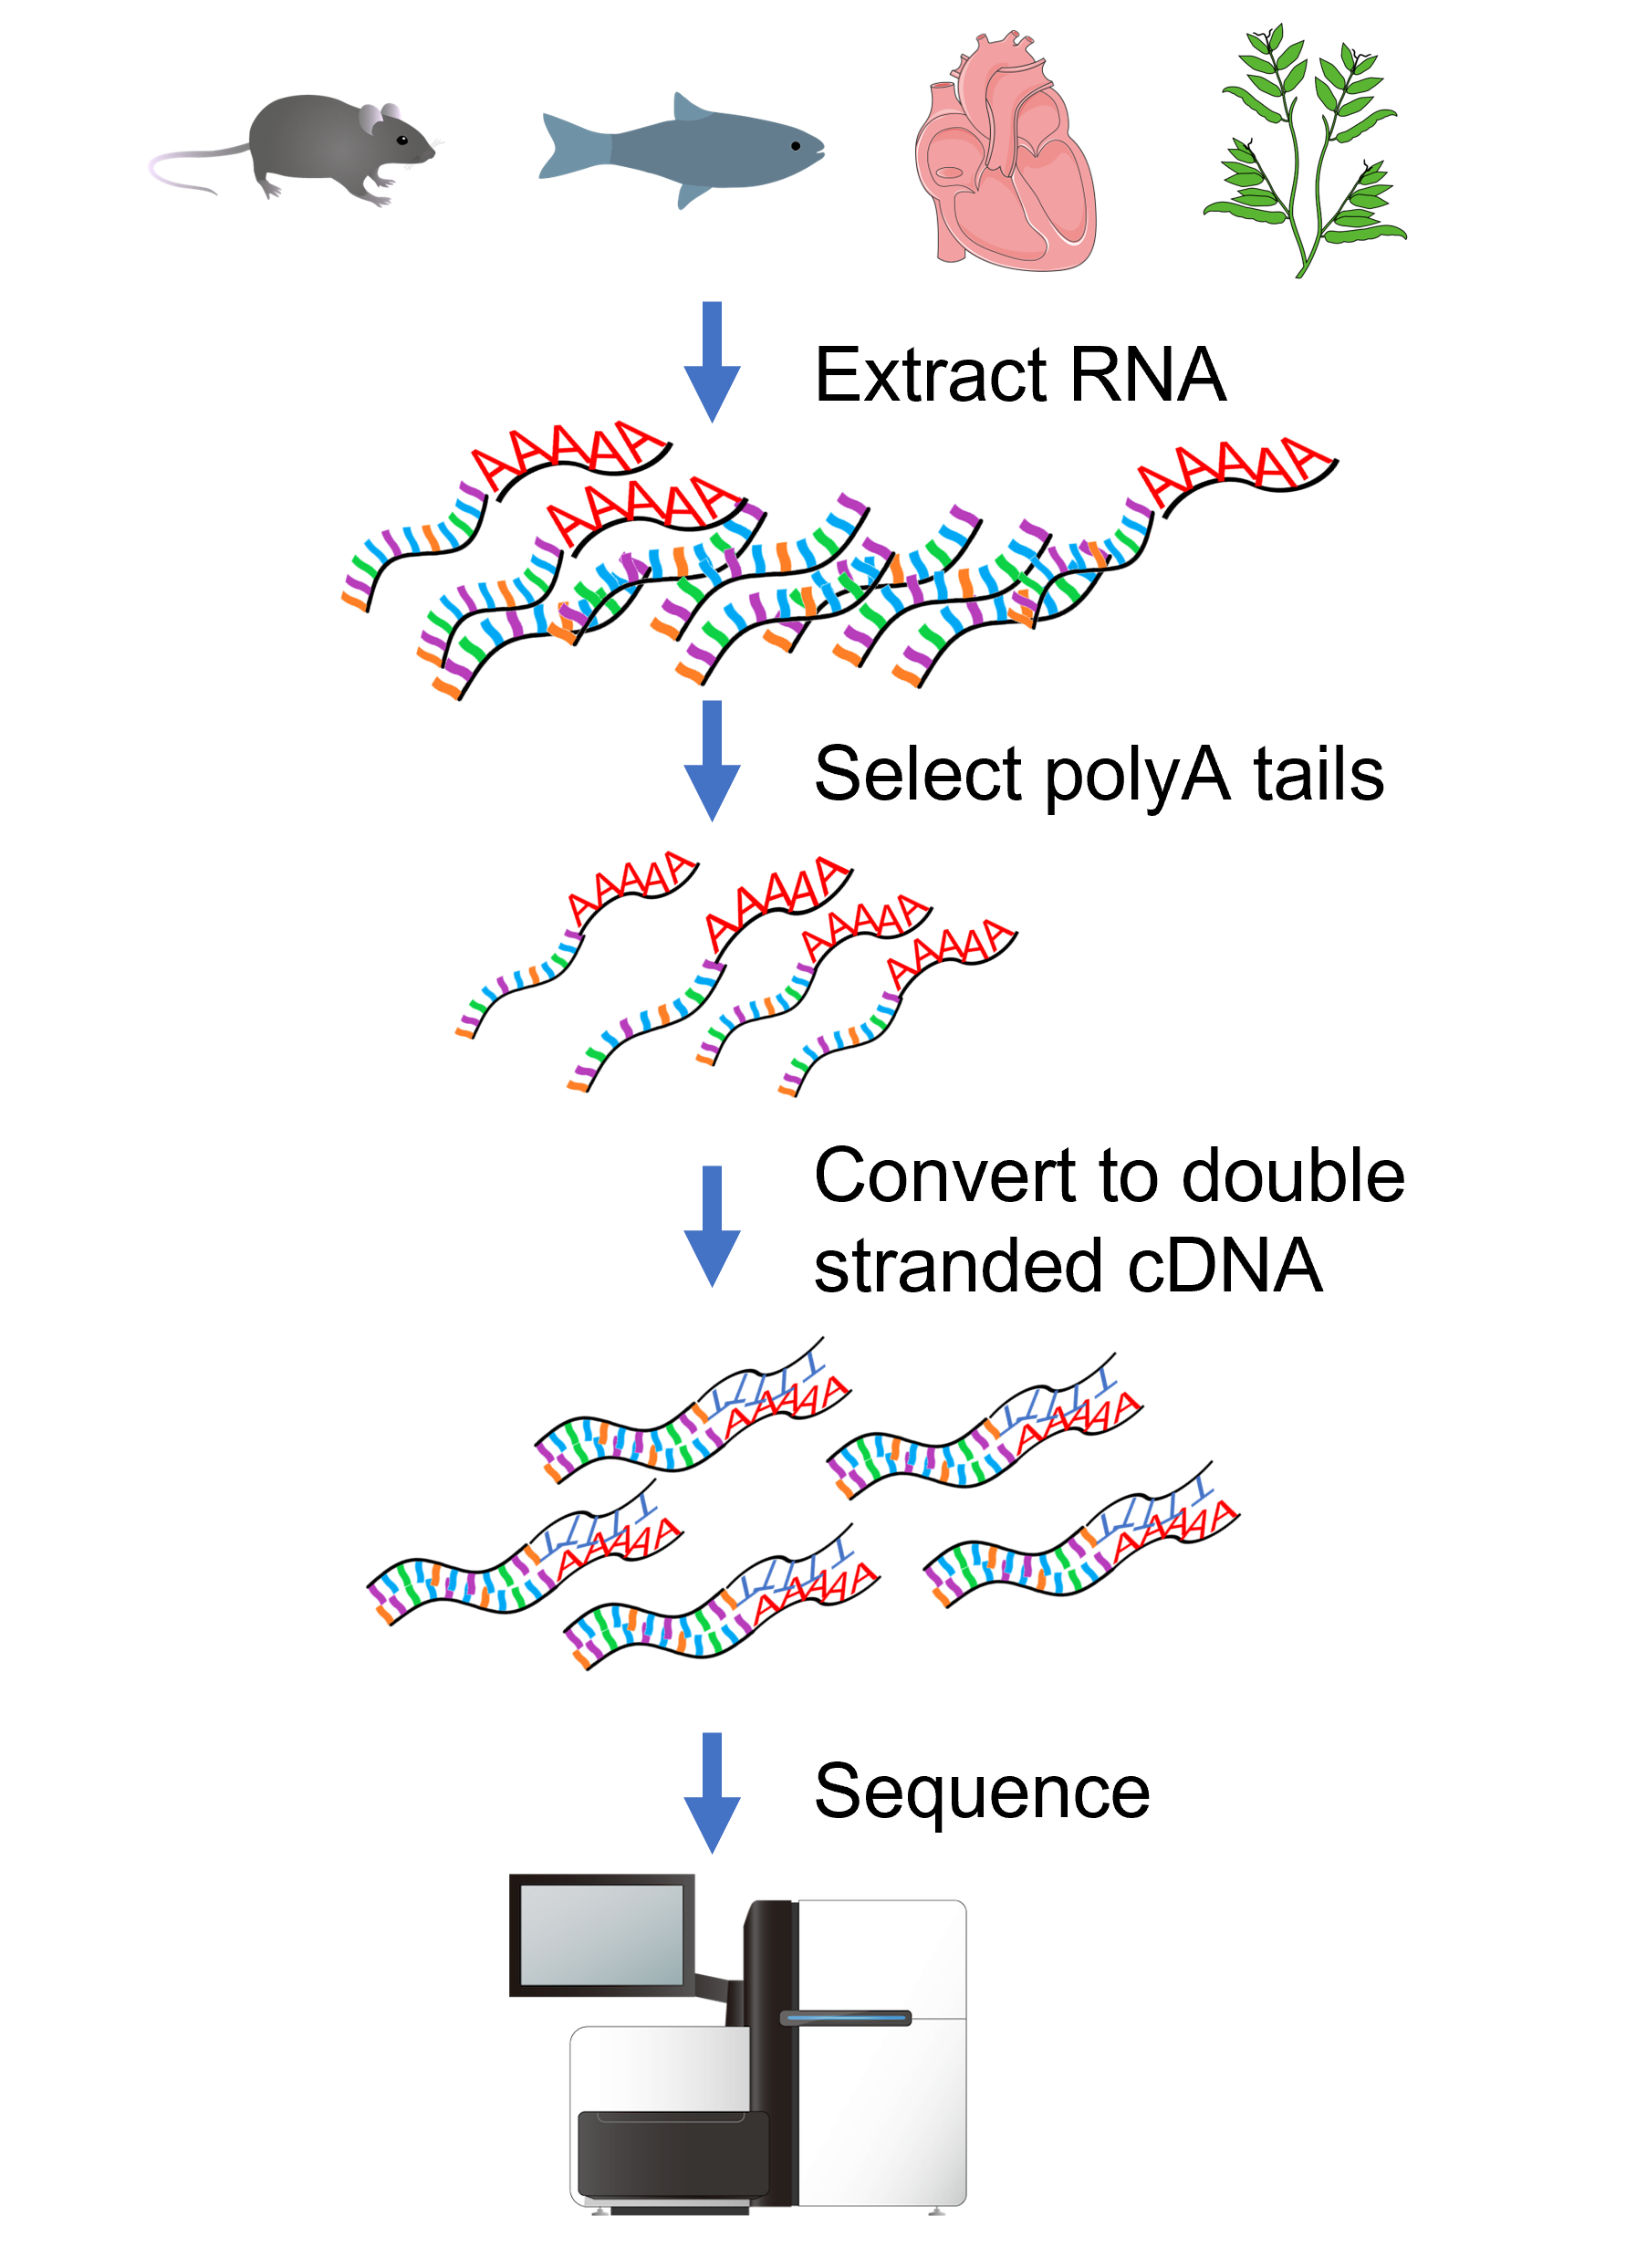
\includegraphics[width=0.4375\linewidth]{files/RNAseq-protocol-5145db85e92cd8e5569c2b42243f6a4e.png}
\caption[]{Standard RNAseq protocol. \newline
Credits: \href{https://creativecommons.org/licenses/by/4.0/}{CC BY 4.0} \cite{own_5_2024} modified/created from \newline
\href{https://creativecommons.org/licenses/by/4.0/}{CC BY 4.0} \cite{RNAseq_seq_2011}, \cite{RNAseq_plant_2023}, \cite{RNAseq_seq_2020}, \href{https://creativecommons.org/licenses/by/3.0}{CC BY 3.0} \cite{RNAseq_mouse_2013}, \cite{RNAseq_heart_2016}, \href{https://creativecommons.org/publicdomain/zero/1.0}{CC0 1.0} \cite{RNAseq_fish_2014}}
\label{RNAseq_protocol}
\end{figure}

The standard protocol of an RNAseq experiment is shown in Figure~\ref{RNAseq_protocol}.
First, all RNA (total RNA) is extracted from a biological sample.
Next, mRNA is selected using a polyT oligo to select RNA with a polyA tail.
The RNA is then converted to stable double stranded cDNA.
The resulting cDNA library is then sequenced, usually as paired end reads of 100-150bp.
A standard sequencing run results in 30 million or more reads per sample.

The read lengths currently used are relatively short and complicated methods
are required to assign reads to exons and isoforms. New developments in this
field are long cDNA conversions that allow sequencing of full-length
transcripts on PacBio and direct sequencing of RNA on Oxford~Nanopore.
This allows the detection of the actual isoforms present in samples.

Next, the reads need to be assigned to their corresponding transcripts. For
this there are two options: mapping of the reads to an existing reference,
which can be either a genome or a transcriptome; or a \textit{de novo} assembly of the
transcripts (similar to assembly of genomes). Once reads have been assigned
to their corresponding transcript or gene, expression is quantified by
counting the number of reads per feature.

The advantage of not using probes (compared to qPCR and microarrays) is that
RNAseq works for species without a reference genome, can identify alternatively spliced
transcripts, SNPs in transcripts, etc. A downside is that usually large
datasets are generated, which require dedicated analysis workflows.


\bigskip
\centerline{\rule{13cm}{0.4pt}}
\bigskip

\subparagraph{Mapping}

In principle, sequenced reads from an RNAseq experiment do not differ from
reads sequenced from genomic DNA in that they can be mapped to a reference
sequence. The same algorithms apply when mapping RNAseq reads to an
assembled transcriptome (a reference sequence that only contains RNA
sequences) or to prokaryotic genomes.

\begin{figure}[!htbp]
\centering
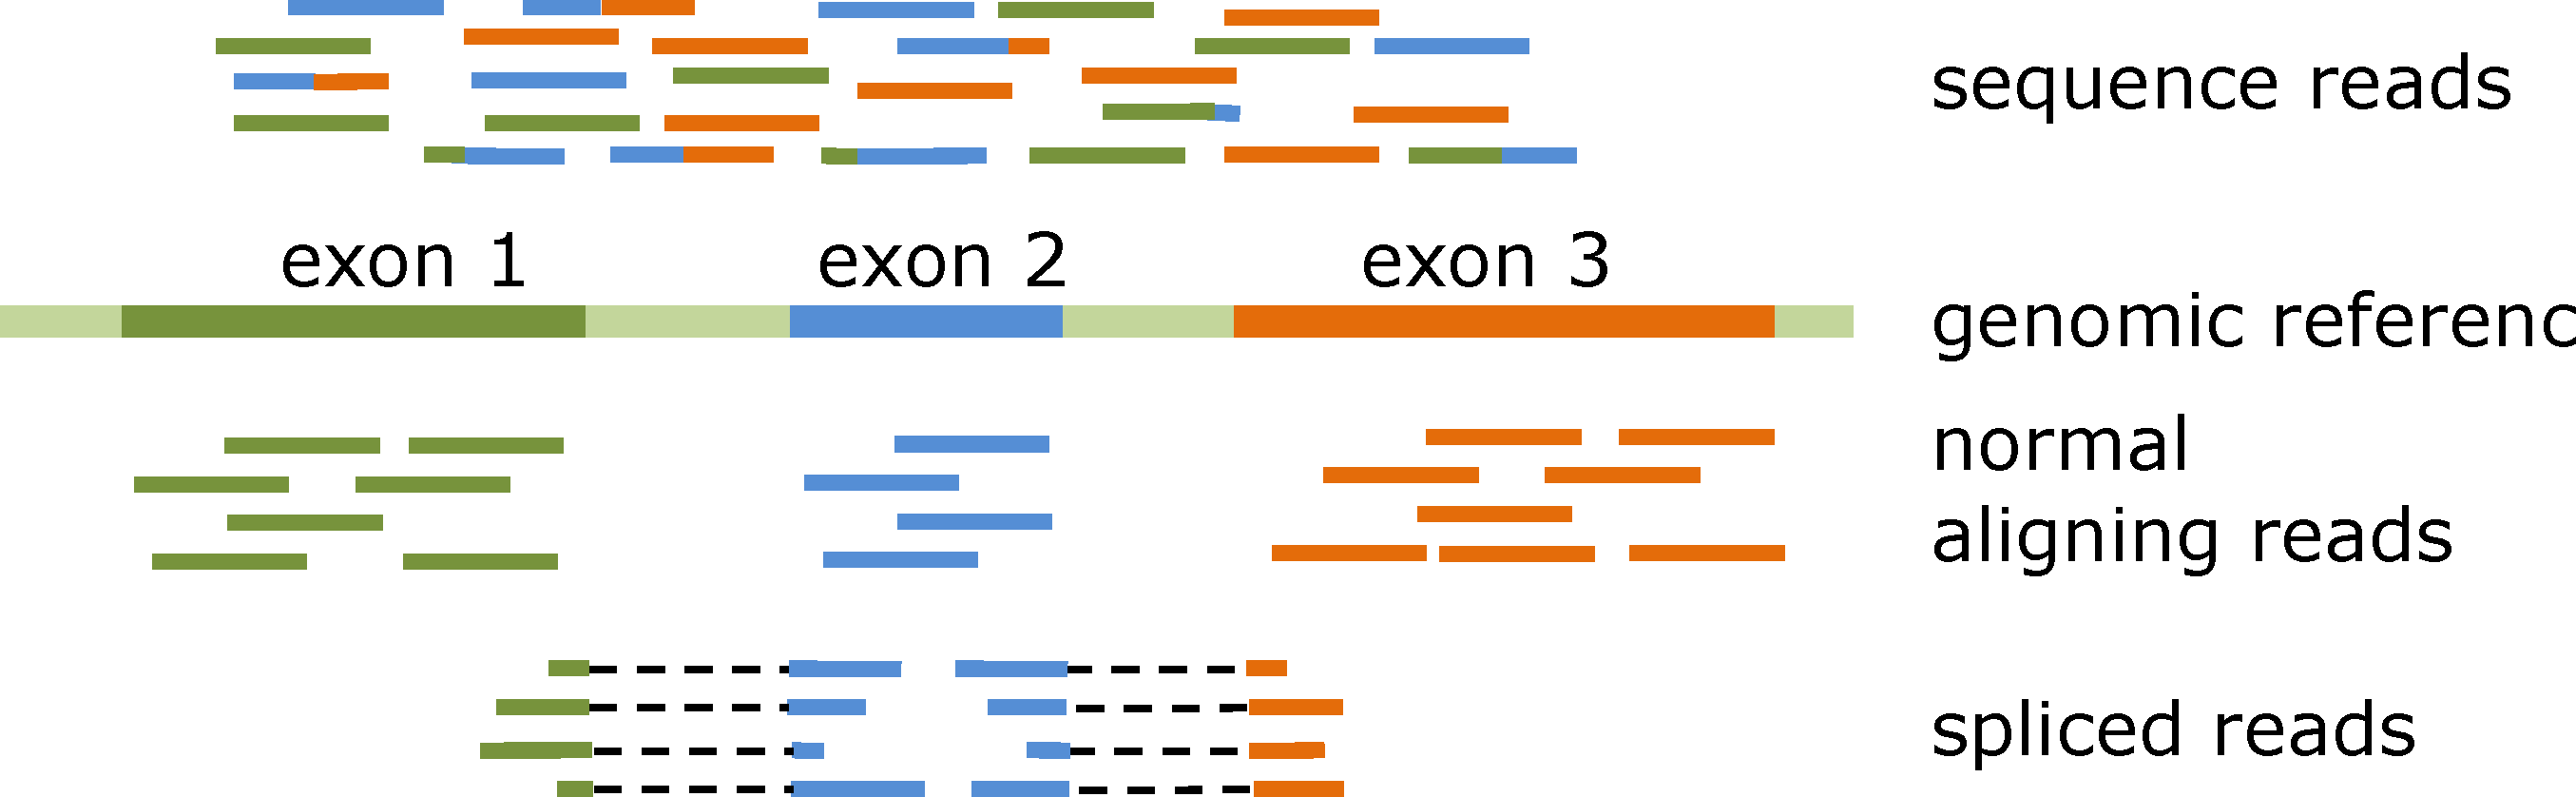
\includegraphics[width=0.7\linewidth]{files/spliced-alignment-1d333f039e966cb4fcf6a3a8946d9099.pdf}
\caption[]{Mapping of mRNA reads to genomic reference with splice aware aligner.
Credits: \href{https://creativecommons.org/licenses/by-nc/4.0/}{CC BY-NC 4.0} \cite{own_5_2024}.}
\label{spliced_alignment}
\end{figure}

Mapping eukaryotic mRNA sequences to a genomic reference is more cumbersome,
as most genes have introns, which are no longer present in the mature mRNA
(Figure~\ref{spliced_alignment}).  This means that reads might contain an
exon-exon junction and should be split along the reference.  Most aligners
will not consider this a valid option.  Special splice-aware aligners have
been developed for this reason, that are able to map normal reads that map
contiguously to the reference sequence as well as reads that are split
across splice sites (Figure~\ref{spliced_alignment}).  They also take into
account known intron-exon boundaries to determine the point within a read
where it has to be split and whether the split alignment is correct.


\bigskip
\centerline{\rule{13cm}{0.4pt}}
\bigskip

\subparagraph{Transcript quantification}

After sequencing and mapping, the next step is to quantify the abundance of
transcripts, i.e., the expression levels. Reads assigned to each feature
(exon or gene) are counted, with the underlying assumption that the number
of reads mapping to a feature is strongly correlated with the abundance of
that feature in the experiment. Comparing abundance of transcripts between
samples, conditions and experiments is not as straight forward as it seems.
Apart from the bullet points above that influence mRNA abundance, there is
variation in each sequencing experiment. The main variation affecting
comparability of read counts between samples is the total number of reads
sequenced in each sample. Also, not all transcripts are the same length,
affecting the number of reads detected per transcript. So, some
normalisation is required to take into account these differences and make
data comparable. The main methods are:

\begin{itemize}
\item \textbf{simple counting}: this is the starting point of every analysis.  We
count the number of reads that map to each exon or gene.


\item \textbf{CPM}: counts per million (reads), a relative measure for
the read counts corrected for the total number of reads of a sample.  It
assigns each read a value that corresponds to the proportion of the total
number of reads that single read represents.  This tiny fraction is then
multiplied by a million to make it more readable.
\end{itemize}

\begin{figure}[!htbp]
\centering
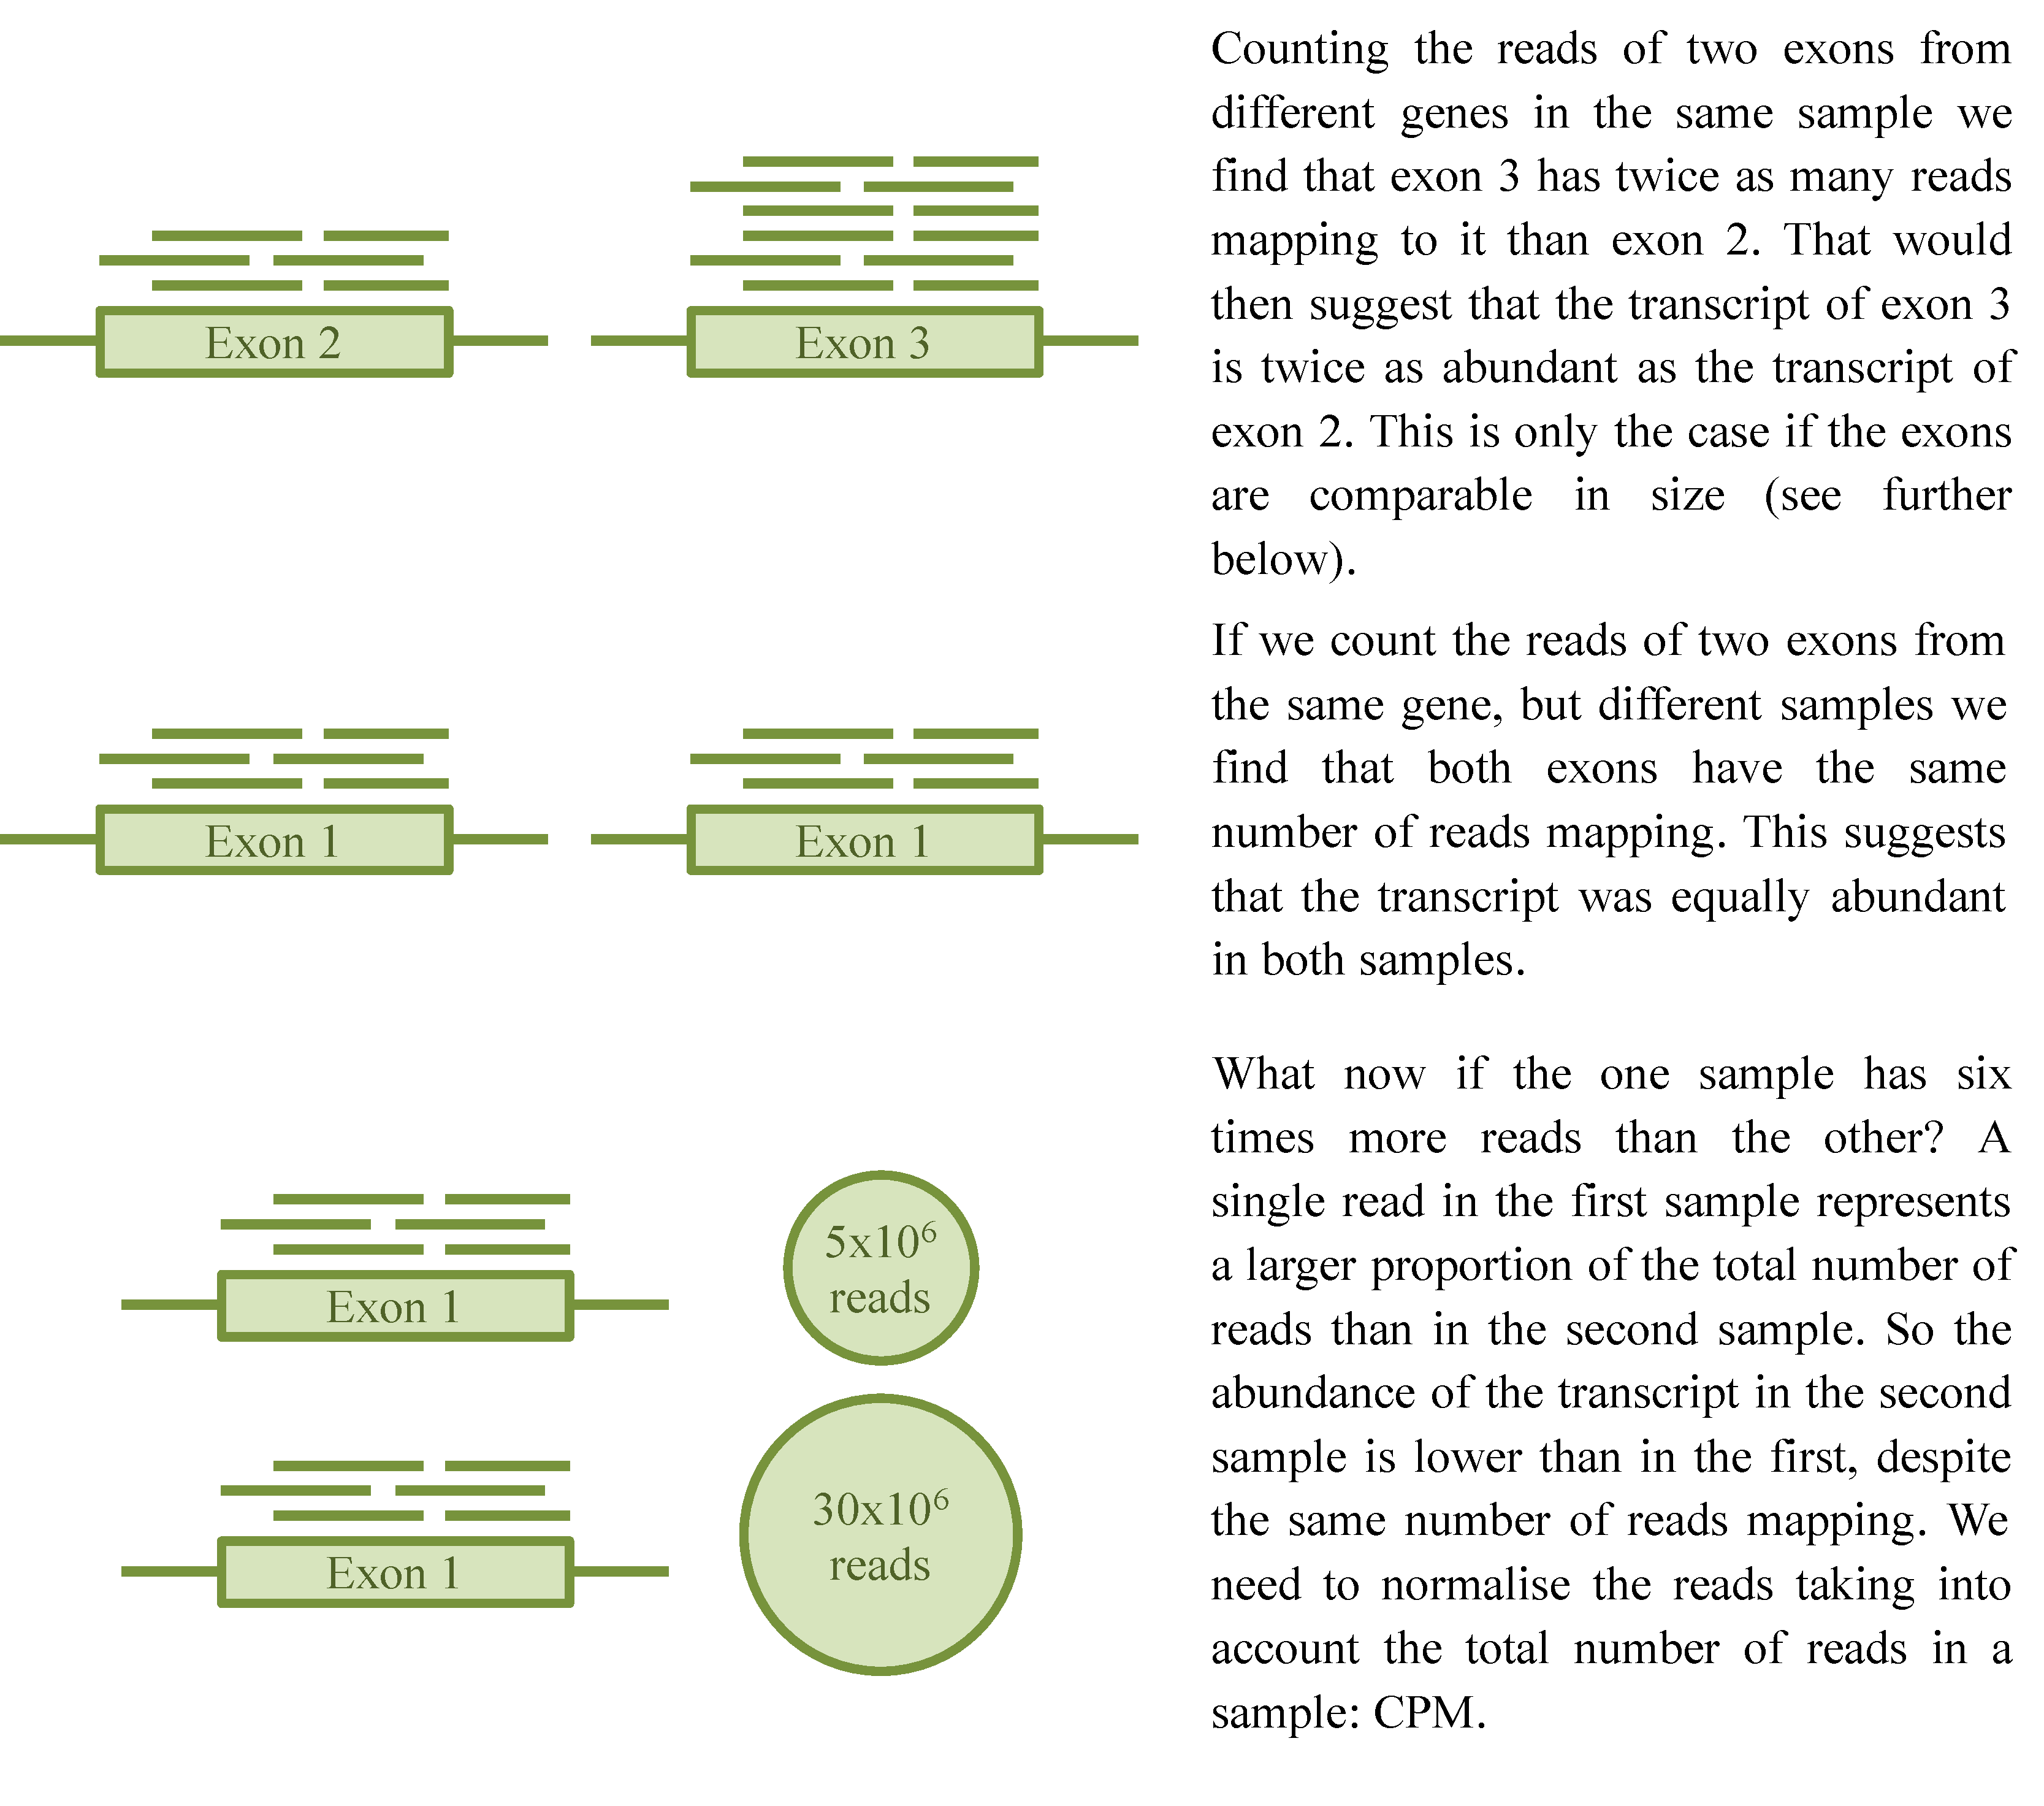
\includegraphics[width=0.7\linewidth]{files/CPM-3324f95a431c80e84eb69a0ecd2711f8.pdf}
\caption[]{Credits: \href{https://creativecommons.org/licenses/by-nc/4.0/}{CC BY-NC 4.0} \cite{own_5_2024}.}
\label{CPM}
\end{figure}

\begin{itemize}
\item \textbf{RPKM, FPKM and TPM}: when comparing expression of two different transcripts, we
also have to take into account the characteristics of the transcripts we
are comparing and normalise accordingly.  RPKM and FPKM (Reads/Fragments
per kilobase transcript per million) normalise the counts per feature
length and the total number of reads.  TPM (transcripts per million
transcripts) normalises per transcript.  TPM uses a calculation to give a
measurement of which proportion of the total number of transcripts in the
original sample is represented by each transcript.
\end{itemize}

\begin{figure}[!htbp]
\centering
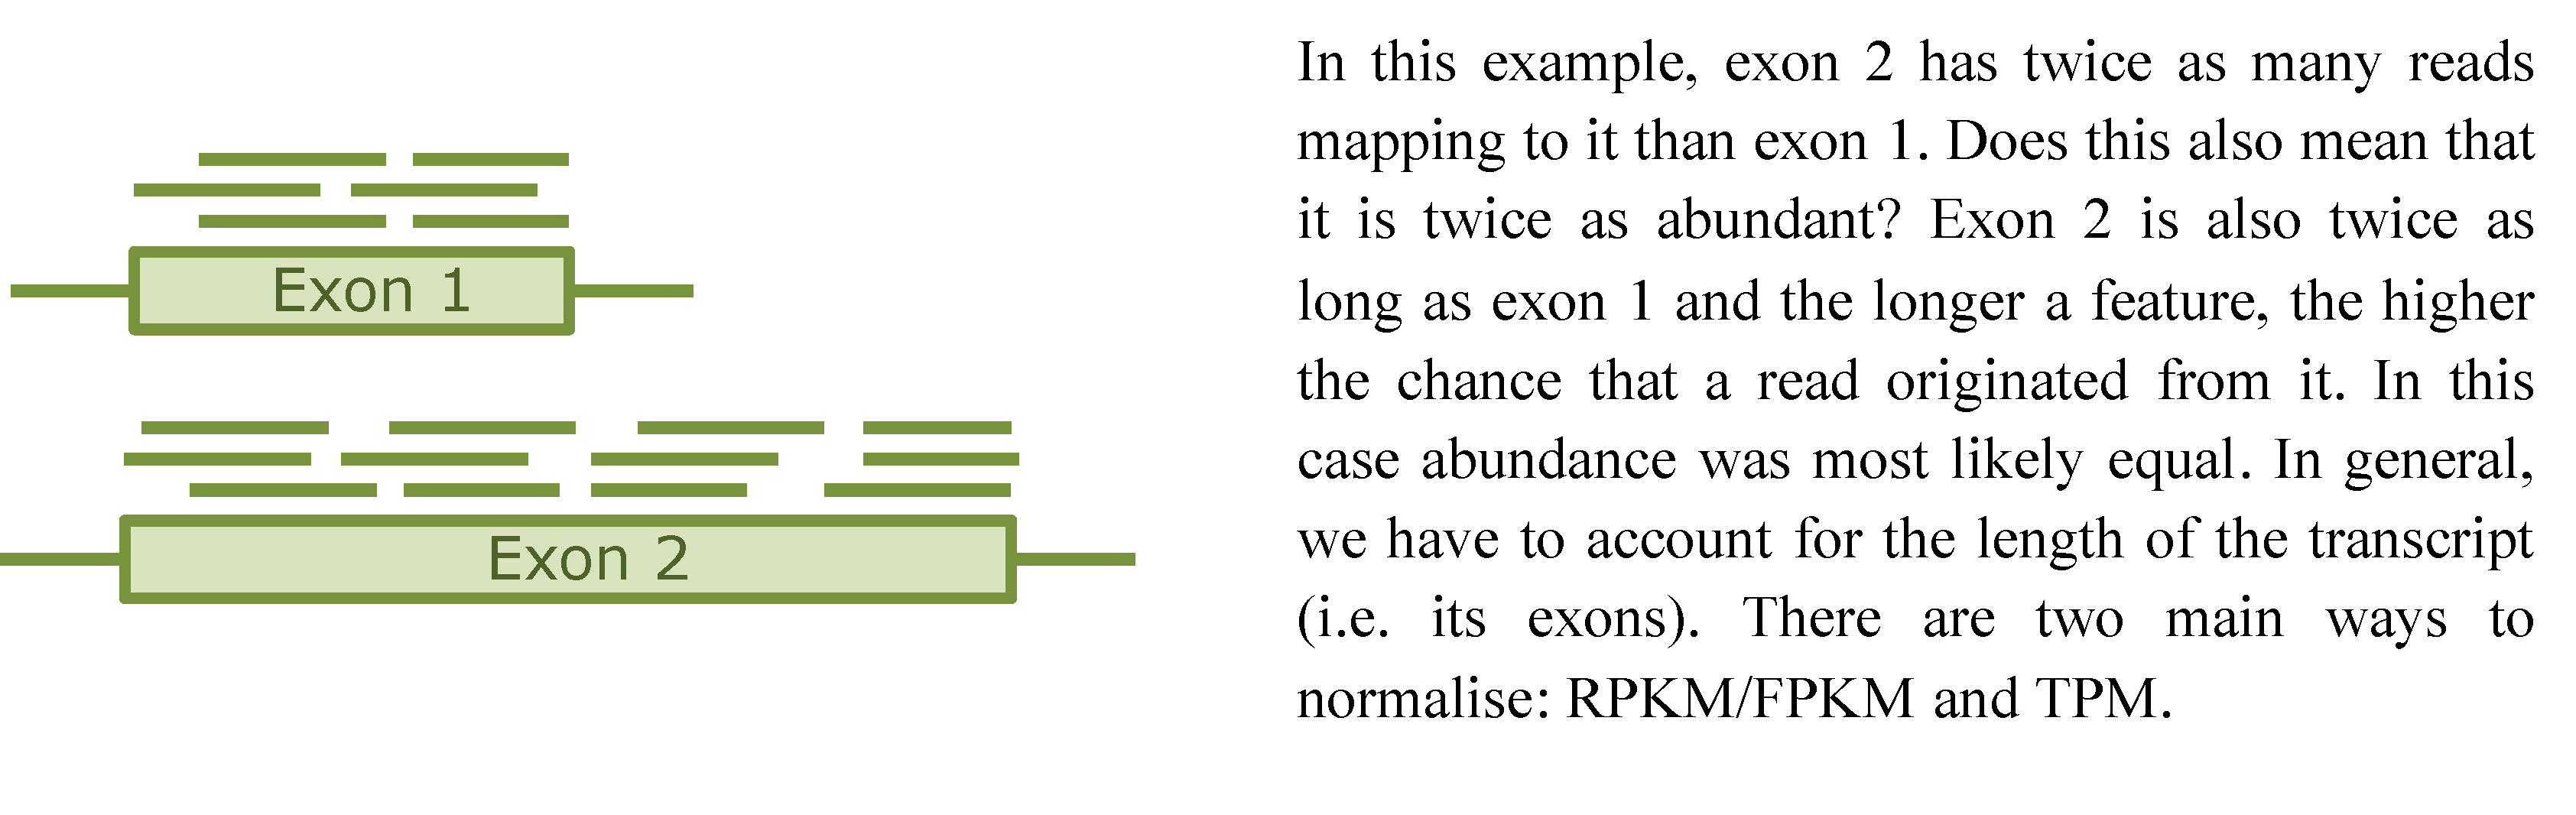
\includegraphics[width=0.7\linewidth]{files/comparing-transcript-2264ff4d41c11a6b0a6f5618c6c83bff.pdf}
\caption[]{Credits: \href{https://creativecommons.org/licenses/by-nc/4.0/}{CC BY-NC 4.0} \cite{own_5_2024}.}
\label{comparing_transcripts}
\end{figure}

There is no clear optimal method, and there is a large debate whether
RPKM/FPKM or TPM are preferred.  CPM can clearly only be used when there is
no difference in transcript length, e.g., when comparing one transcript
between two samples.

\begin{framed}
\textbf{Box 5.13: Ever more detail}\\
Until now, most RNAseq experiments have been performed on groups of cells,
as sequencing devices require large amounts of DNA. This means that cells
of different cell types or different life stages are included in a single
sample. While detection of differentially expressed genes is clearly
possible with this method, weak or more nuanced variation is averaged out
across all cells. Recently, methods have become available that separate
tissues into individual cells and sequence each of these separately. This
does require PCR amplification of RNA to reach the amounts required for
sequencing, as well as sophisticated bioinformatics and statistical methods
to deal with the resulting data. Other recent technology allows to measure
transcription spatially (e.g. in a tissue), at specific locations on a grid.
For a review on single-cell transcriptomics, see this
\cite{Bacher_2016};
a recent review on spatial transcriptomics can be found
\href{https://www.nature.com/articles/s41587-022-01448-2}{here}.
\end{framed}


\bigskip
\centerline{\rule{13cm}{0.4pt}}
\bigskip

% #### ChIPseq and other protocols
% 
% :::{figure} images/chapter5/chip-protocol_alt.jpg
% :alt: ChIPseq protocol
% :align: center
% :name: chip_protocol_alt
% 
% The chromatin immunoprecipitation (ChIP) protocol. Proteins are
% cross-linked to DNA, after which genomic DNA is isolated and sheared. Using
% an antibody, only the protein of interest is selected (the
% immunoprecipitation step), after which the cross-linking is reversed and the
% DNA can be sequenced by PCR (ChIP-PCR) or NGS (ChIPseq). Similar protocols
% are available for protein-RNA and protein-protein interactions, the latter
% using two antibodies.
% Credits: [CC BY 4.0](https://creativecommons.org/licenses/by/4.0/) {cite}`chip_protocol_alt_2015`.
% :::
% 
% RNAseq is a clever protocol that uses the attractive cheap, high-throughput
% DNA sequencing technology to measure something else – in this case, gene
% expression levels. The trick is to first translate the mRNA into DNA,
% measure the DNA, and then reconstruct the desired measurement by transcript
% quantification. Many more such protocols have been developed to measure
% other molecule levels and interactions of interest. Three well-known
% protocols are:
% 
% - ChIPseq, for chromatin immunoprecipitation sequencing: for a given protein
%   – for example, a transcription factor or a histone – this can detect where
%   it binds DNA.
%   {numref}`chip_protocol_alt` illustrates this.
%   After sequencing, the DNA can be mapped against the genome: peaks of mapped
%   reads indicate regions where the protein of interest binds.
% - Hi-C, to study 3D proximity of chromosome parts in the nucleus.
% - Bisulfite sequencing, to assess methylation of DNA.


\bigskip
\centerline{\rule{13cm}{0.4pt}}
\bigskip

\paragraph{Proteomics}\label{chapter5_proteomics}

As mentioned earlier, transcriptomics is widely applied but does not reflect
the overall cellular state accurately. The resulting proteins are the workhorses
of the cell, and knowing their concentrations, modifications and
interactions provides more insight than gene expression can provide.
Unfortunately, while major advances have been made in proteomics
technologies, accurate measurement of proteins is still complex and costly,
for a number of reasons:

\begin{itemize}
\item Obviously, the problem of identifying molecules with 20 building blocks
(amino acids) is harder than that of identifying molecules with 4 building
blocks (nucleotides).
\item Moreover, given alternative splicing, the number of proteins that needs to
be distinguished is higher than the number of genes.
\item Proteins can be modified in a myriad of ways after translation, structurally, as well as
biochemically, by the addition of many different groups on individual amino
acids. For some proteins, it is estimated that many thousands of different
variants can be found in a cell.
\item Most proteins are structured, some form complexes or insert into the
membrane; such structures often have to be removed to allow accurate measurements.
\item Proteins lack properties that make DNA and RNA easy to multiply (PCR) and measure:
replication and binding to complementary strands.
\item The dynamic range of protein abundances is enormous: some protein
concentrations are a million-fold higher than that of others. This would
not be a problem if we had a protocol to make copies of low-abundant
proteins (like PCR for DNA), but such a protocol is not available.
\end{itemize}

Still, a number of methods to measure proteins and their interactions are in
use. We distinguish between quantitative proteomics (measuring
presence/absence and levels of proteins) and functional proteomics
(measuring protein interactions with other molecules).


\bigskip
\centerline{\rule{13cm}{0.4pt}}
\bigskip

\subparagraph{Quantitative proteomics}

\begin{framed}
\textbf{Box 5.14: Mass spectrometry}\\
Mass spectrometry (MS) devices have been in constant development and
improvement since their inception in the late 19\textsuperscript{th} century.  They
differ in specific setup, but all follow three basic steps:

\begin{enumerate}
\item Ionize a molecule.
\item Separate or select molecules based on their mass.
\item Detect time and/or location of arrival at a detector to infer the mass of
each molecule.
\end{enumerate}

To be fully correct, MS measures the mass-over-charge ratio (m/z) rather
than the actual mass, i.e., the mass in relation to the charge number of the
ion.

For each step, different technologies are available which are best suited to
detection of specific mixtures, compounds of interest (proteins, metabolites),
and compound size ranges. Figure~\ref{mass_spectrometry_alt} illustrates a number of widely used
separation steps, i.e., by measuring time-of-flight or susceptibility to
deflection by magnetic fields or by tuning an oscillating electrical field
to allow only specific masses to pass through.

% :::{figure} images/chapter5/mass-spectrometry.png
% :alt: Three mass spectrometry setups
% :align: center
% :name: mass_spectrometry
% 
% Three mass spectrometry setups, (a) time-of-flight,
% (b) sector field and \(c) quadrupole. Credits: {cite}`mass_spectrometry_2003`.
% :::
% #% Unable to use figure mass_spectrometry due to copyright.

\begin{figure}[!htbp]
\centering
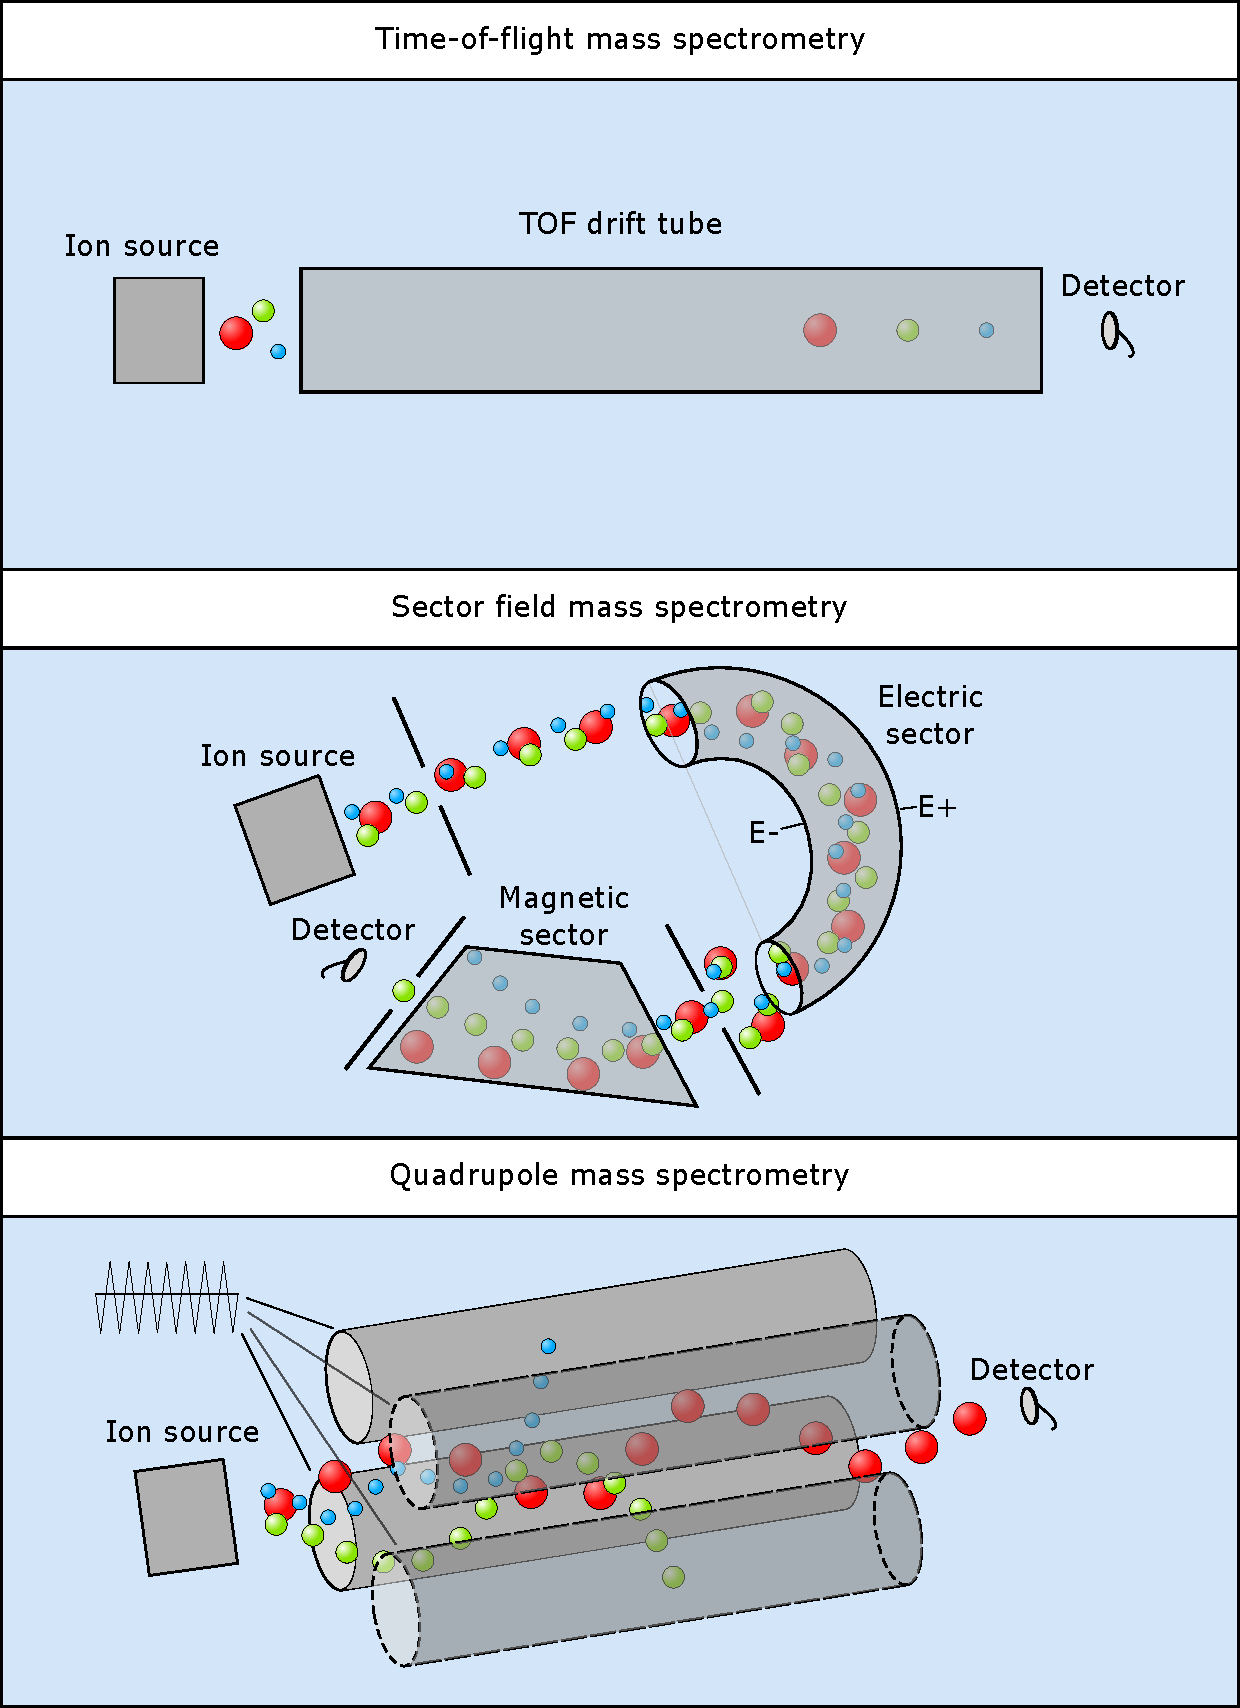
\includegraphics[width=0.7\linewidth]{files/mass-spectrometry_al-ef48fd26c793a2135d7e8d5362597800.pdf}
\caption[]{Three mass spectrometry setups, (top) time-of-flight,
(middle) sector field and (bottom) quadrupole.
Credits: \href{https://creativecommons.org/licenses/by-nc/4.0/}{CC BY-NC 4.0} \cite{own_5_2024}.}
\label{mass_spectrometry_alt}
\end{figure}

\begin{figure}[!htbp]
\centering
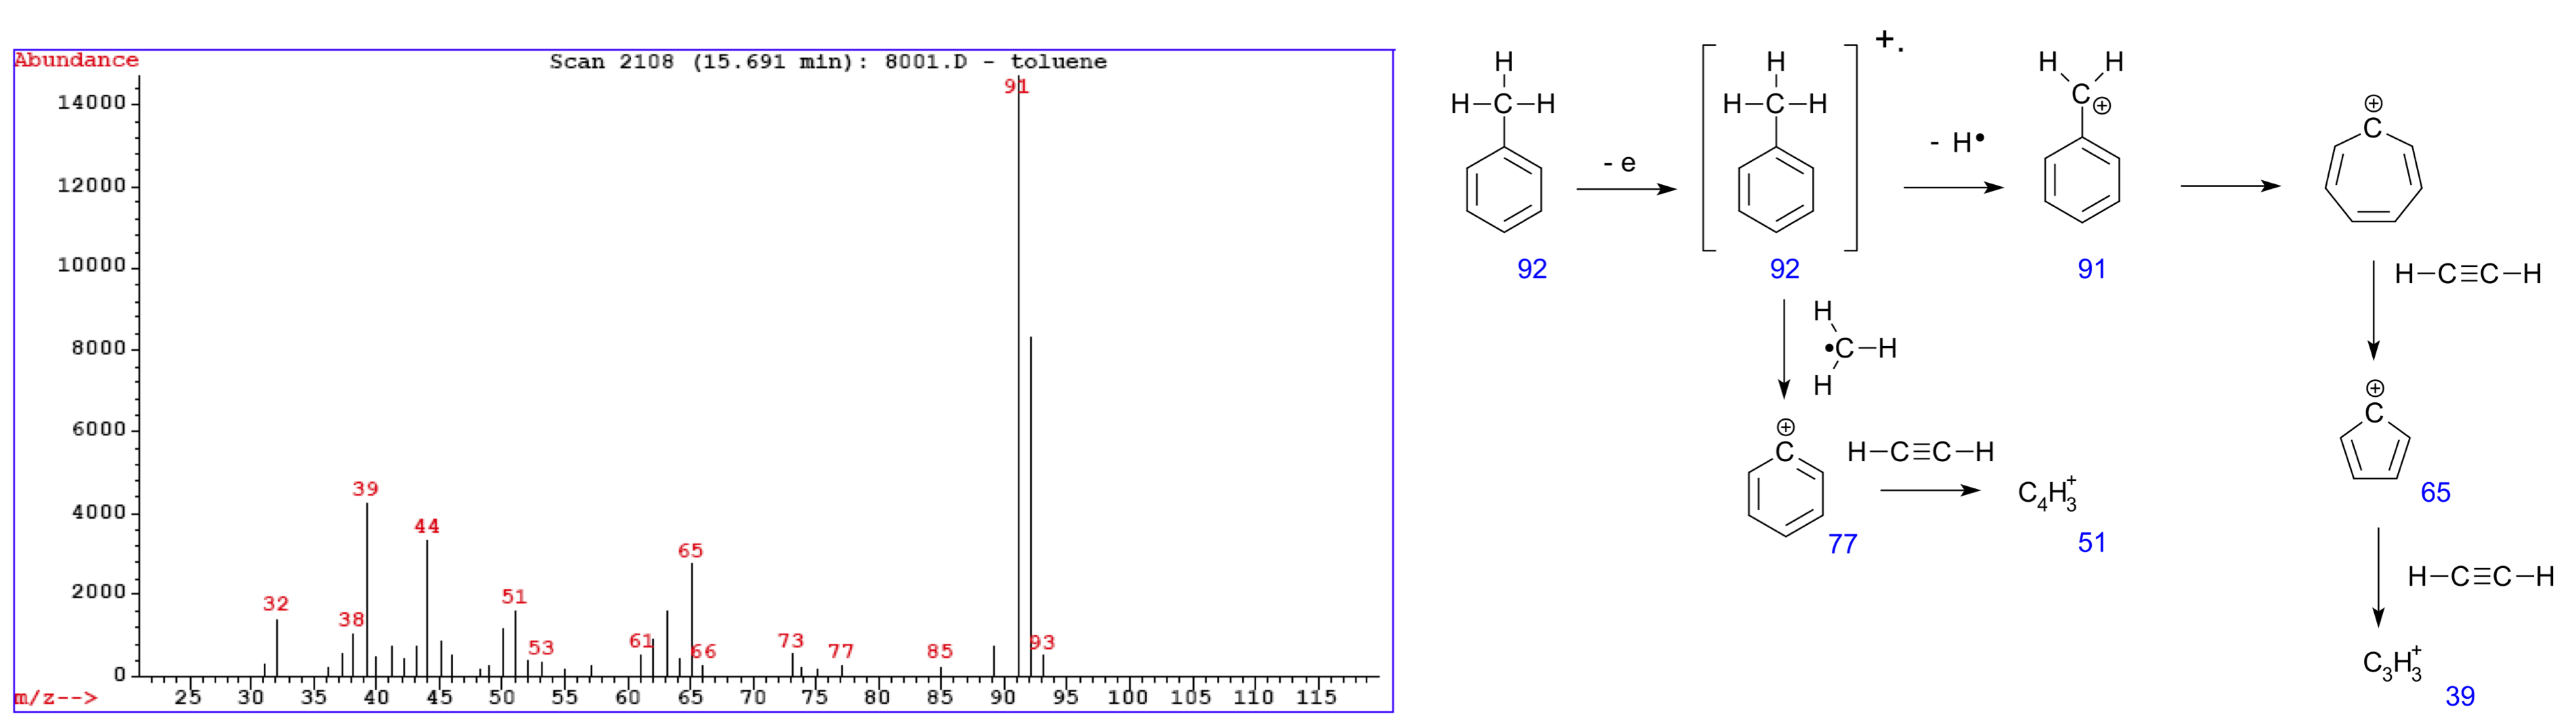
\includegraphics[width=0.7\linewidth]{files/mass-spectrum-38bac03b7ea6e4b7427b61567e2f2ef9.png}
\caption[]{An example mass spectrum measured on toluene (left). The various peaks
correspond to fragments of the original molecule (right).
Credits: modified from (left) \href{https://creativecommons.org/licenses/by-sa/3.0/}{CC BY-SA 3.0} \cite{mass_spectrum_left_2005}, (right) \href{https://creativecommons.org/licenses/by-sa/3.0/}{CC BY-SA 3.0} \cite{mass_spectrum_right_2008}.}
\label{mass_spectrum}
\end{figure}

The output of any MS experiment is a mass spectogram, with m/z
ratios on the x-axis and peaks indicating how many molecules of a certain
mass have been detected (Figure~\ref{mass_spectrum}).
\end{framed}

In theory, if a database of known
molecule structures (e.g., proteins or peptides) and their calculated masses
would be available, one could look up each mass and identify the
corresponding molecule. A major challenge in interpreting such a
spectrum is the limited resolution of MS devices, which means that a
certain peak can still be caused by many different types of molecules. Some
smaller molecules of interest may even have identical masses (e.g.,
isoforms) and so cannot be distinguished, which is particularly hard in
complex mixtures. A number of approaches try to solve this problem:

\begin{itemize}
\item Chromatography: moving the sample through a separation column before entering the MS
device, filled with an inert gas (gas chromatography, GC) or liquid
(liquid chromatography, LC). Different molecules take different times to travel through these
columns, and arrival time at the MS device thus provides extra information.
\item Tandem mass spectrometry or MS/MS: measuring molecules twice, once intact (in a first MS device) and then
again after selection and fragmentation (in a second MS device). This depends on the
predictability of fragmentation: if a molecule falls apart at specific
places, we can get more information from the combination of the overall mass
and the masses of the fragments it breaks into.
\item Shotgun proteomics: specifically for proteins, a protocol in which an enzyme is first used to
cut the protein at specific places (for example, trypsin cleaves the protein
into peptides at arginines and lysines) (Figure~\ref{shotgun_proteomics_alt}). The peptide masses are then
measured and compared to the mass spectra of predicted peptides resulting from a
database of known proteins, to identify the protein likely being measured.
This approach can also be used to measure posttranslation modifications,
as they lead to small (known) shifts in the measured spectra for the modified
peptides.
\end{itemize}

\begin{figure}[!htbp]
\centering
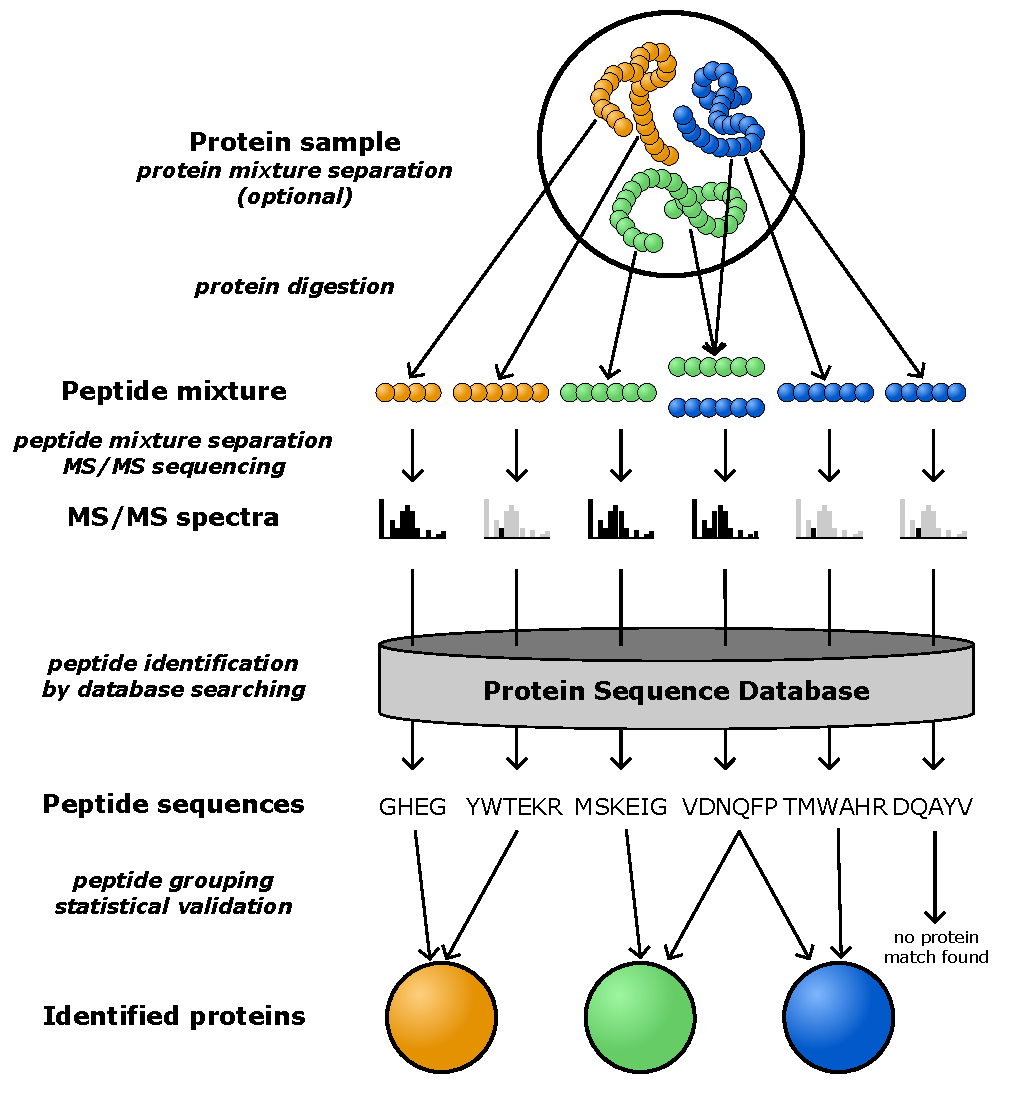
\includegraphics[width=0.7\linewidth]{files/shotgun-proteomics_a-8030910a3755a6cc3057d2e5f5162fc9.pdf}
\caption[]{A schematic overview of shotgun proteomics.
Credits: \href{https://creativecommons.org/licenses/by/4.0/}{CC BY-NC 4.0} \cite{own_5_2024}.}
\label{shotgun_proteomics_alt}
\end{figure}

\subparagraph{Functional proteomics}

Next to protein levels, we are also interested in what proteins do in the
cell: their functions and interactions. Many protocols and analyses have
been developed for this, with most focusing on protein-protein, protein-DNA
and protein-metabolite (enzymatic) interactions. Box~5.14 lists some methods to
measure such interactions. Note that while many of these experiments are
cumbersome, they are essential to advance functional genomics -
(bioinformatics) predictions critically depend on high-quality data and
cannot replace experimental validation.

\begin{framed}
\textbf{Box 5.14: Measuring functional interactions}\\
\begin{figure}[!htbp]
\centering
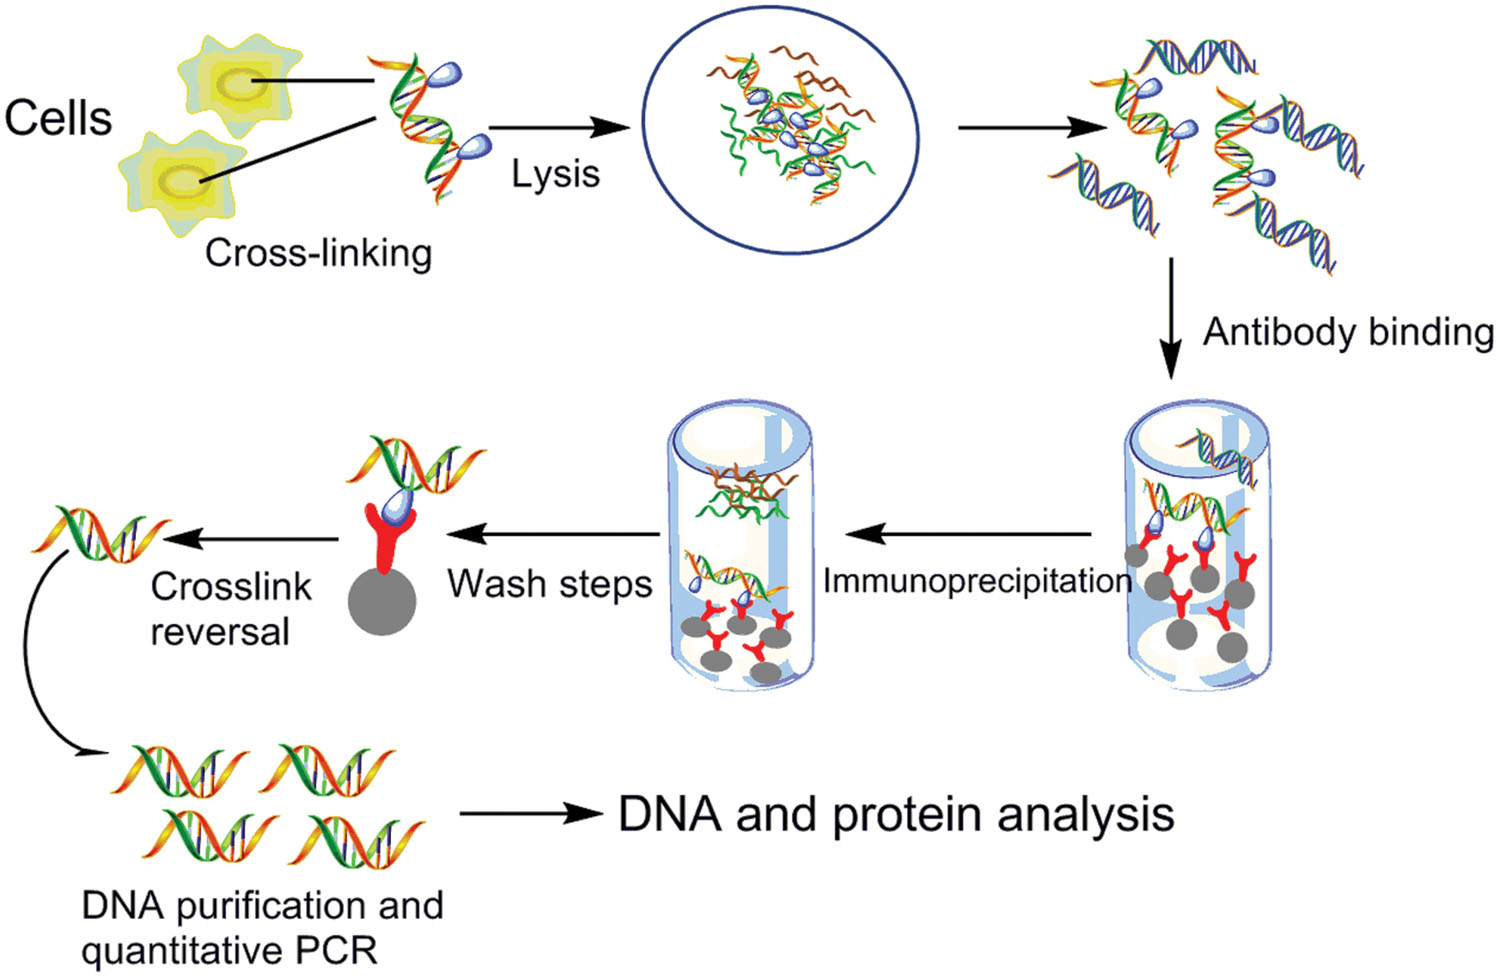
\includegraphics[width=0.7\linewidth]{files/chip-protocol_alt-a399ea3b54d09e8950dfaf488d2396de.jpg}
\caption[]{The chromatin immunoprecipitation (ChIP) protocol. Proteins are
cross-linked to DNA, after which genomic DNA is isolated and sheared. Using
an antibody, only the protein of interest is selected (the
immunoprecipitation step), after which the cross-linking is reversed and the
DNA can be sequenced by PCR (ChIP-PCR) or NGS (ChIPseq). When reads are then
mapped on the genome, peaks indicate where proteins are bound.
Credits: \href{https://creativecommons.org/licenses/by/4.0/}{CC BY 4.0} \cite{chip_protocol_alt_2015}.}
\label{chip_protocol_alt}
\end{figure}

For protein-DNA interaction, the ChIPseq method
(Figure~\ref{chip_protocol_alt}) uses RNAseq to learn how proteins modify DNA,
initiate replication and repair, and regulate expression as transcription
factors or enhancers.

\begin{figure}[!htbp]
\centering
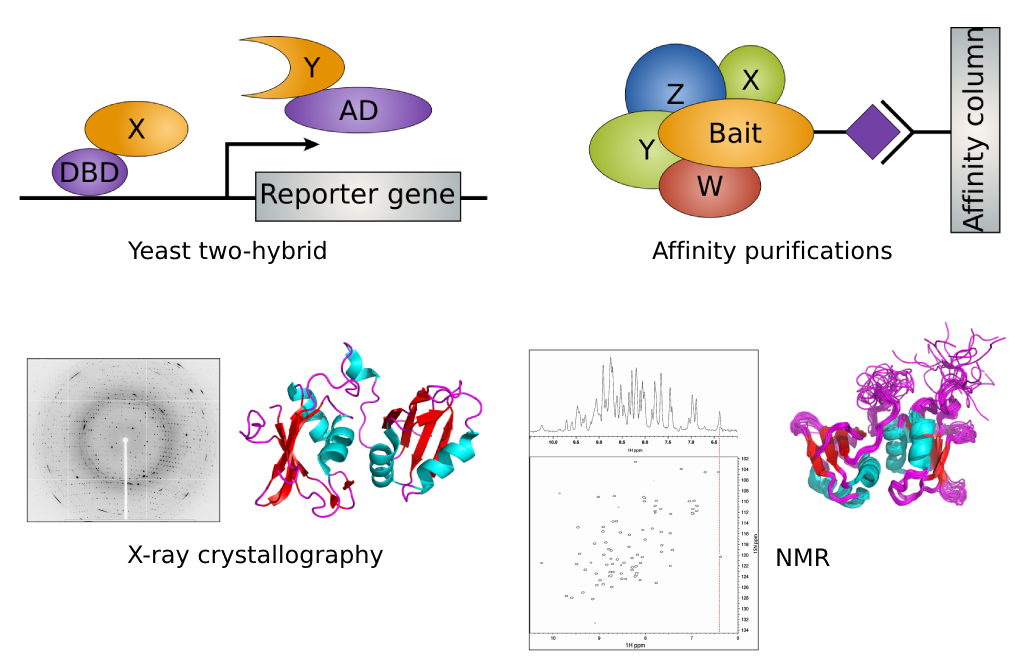
\includegraphics[width=0.7\linewidth]{files/experimental-protein-ac5d5340137b8cc795b520a62aadbf03.png}
\caption[]{Experimental methods to detect proteins. Top: high-throughput, bottom: low-throughput.
Credits: \href{https://creativecommons.org/licenses/by/4.0/}{CC BY-NC 4.0} Top: \cite{own_5_2024}. Bottom: \cite{experimental_protein_methods_bottom_alt_nd}.}
\label{experimental_protein_methods_alt}
\end{figure}

For protein-protein interactions, the main high-throughput protocols
(Figure~\ref{experimental_protein_methods_alt}, top) are:

\begin{itemize}
\item Yeast two-hybrid, in which one of the two proteins is attached to a DNA-binding
domain and the other to an expression activating domain. Only if the two
proteins interact will a reporter gene (e.g., for a fluorescent protein) be
expressed.
\item Tandem affinity purification, in which all proteins interacting with a
``bait'' protein are purified and subsequently measured using MS.
\end{itemize}

These protocols are noisy and have many false positives and negatives, so
further experimental validation using low-throughput methods, essentially
measuring the structure of protein complexes, is often necessary
(Figure~\ref{experimental_protein_methods_alt}, bottom).

Very recently, \href{https://www.nature.com/articles/s41586-024-07487-w}{AlphaFold 3} has been introduced, which promises to predict
interactions between proteins and other proteins, DNA, small molecules etc.
computationally (like AlphaFold 2 predicts protein structure). However, it
still has to be seen whether this tool is reliable enough in practice; the
fact that it is not fully available to the public does not make that very
easy.
\end{framed}

Like transcriptomics data, ``interactomics'' measurements are stored in
databases, such as \href{https://www.ebi.ac.uk/intact/home}{IntAct}, and can be
used to obtain insights into cell-wide protein interaction networks
(Figure~\ref{protein_network}).  Groups of highly connected proteins, i.e.,
with many interactions, can indicate e.g. protein complexes or signalling
pathways within or between cells; protein-DNA relations can be used to
identify gene expression regulation programmes.

Note that the methods mentioned measure \textit{physical} interactions between
proteins, as opposed to \textit{functional} interactions.  Such interactions occur
when two proteins have similar functions - even though they may never
actually physically interact, for example when they are two alternative
transcription factors for the same gene.  Such functional interactions can
be measured to some extent, but are mostly predicted by bioinformatics tools
that combine various pieces of evidence: literature, sequence similarity,
gene co-expression, etc.  \href{https://string-db.org/}{STRING} and
\href{https://genemania.org/}{GeneMania} are the most well-known examples.

\begin{figure}[!htbp]
\centering
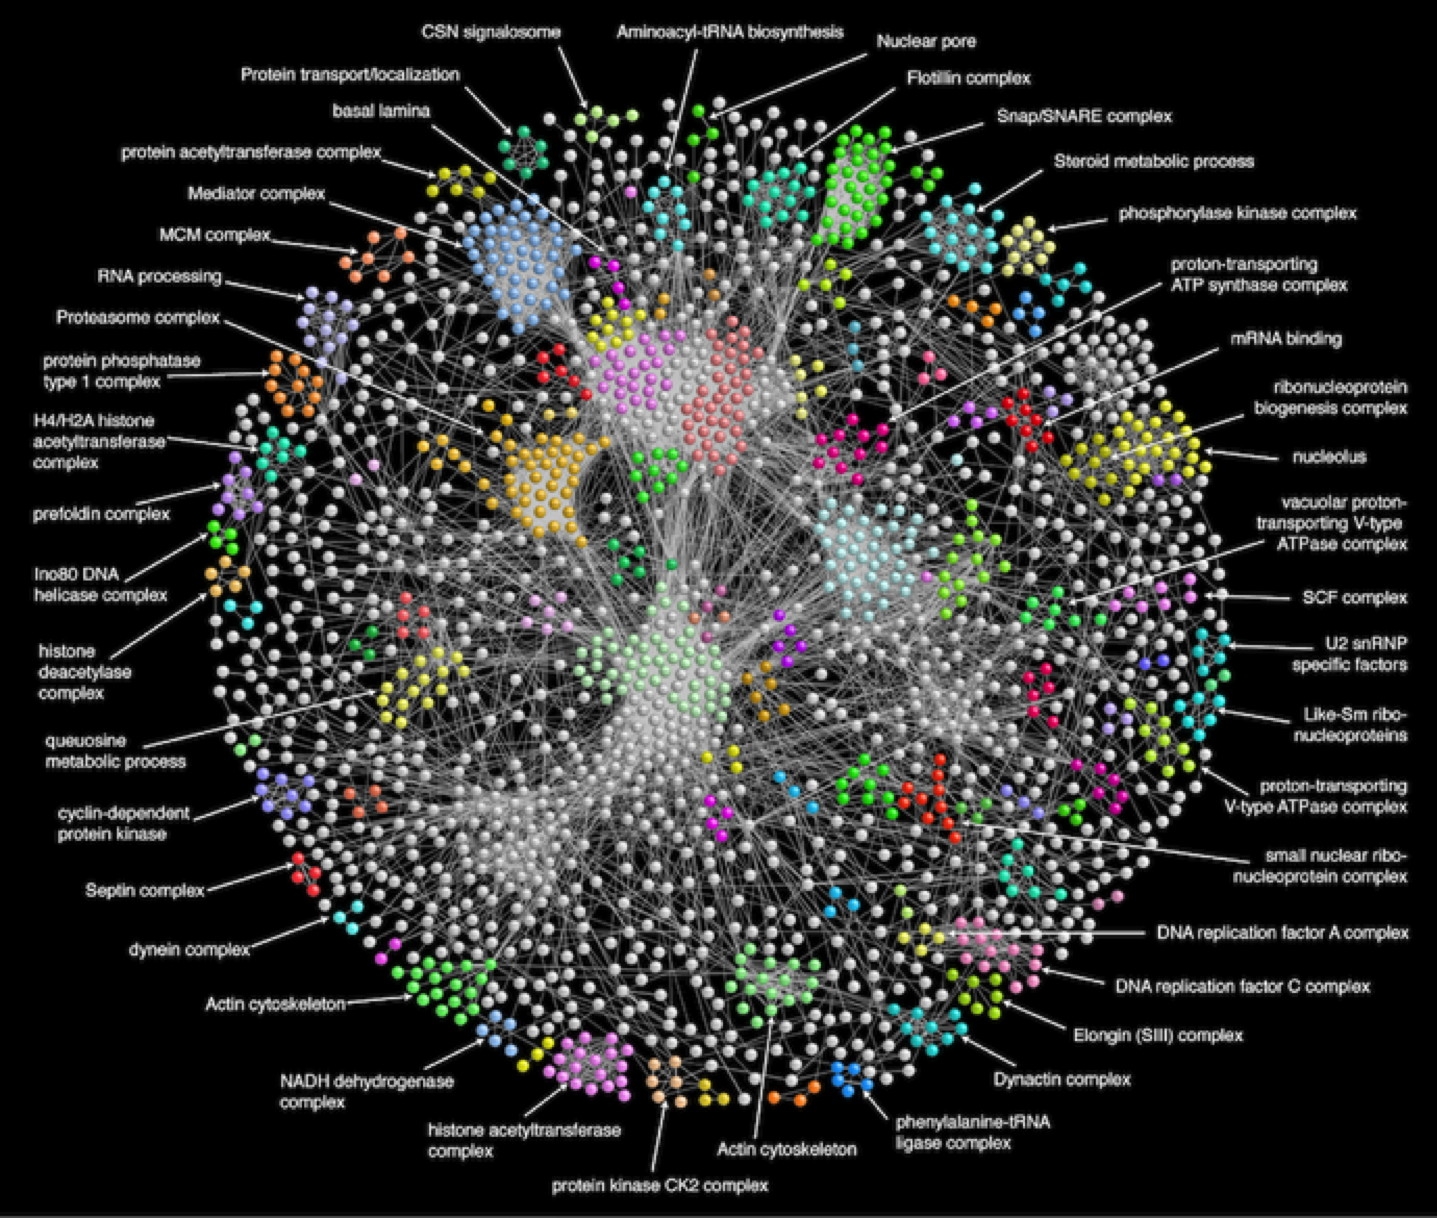
\includegraphics[width=0.7\linewidth]{files/protein-network-c644481d7faaea1cd035f0142131c3bb.jpg}
\caption[]{A protein interaction network (4,927 proteins, 209,912 interactions found by
tandem affinity purification) for \textit{Drosophila melanogaster}, with
clusters corresponding to protein complexes indicated in color.
Credits: modified from \cite{protein_network_2011} under \href{http://www.elsevier.com/open-access/userlicense/1.0/}{Elsevier user license}.}
\label{protein_network}
\end{figure}

% #% Figure protein_network is under open access: Permitted for non-commercial purposes: read, print & download. We should be able to use this image.


\bigskip
\centerline{\rule{13cm}{0.4pt}}
\bigskip

\paragraph{Metabolomics}

\begin{figure}[!htbp]
\centering
\includegraphics[width=0.7\linewidth]{files/metabolic-network-7962579ace4aebf673a1c3d3d185db39.png}
\caption[]{The Roche biochemical pathway chart: global overview of metabolic processes
(left) and a close-up of part of the citrate cycle (right).
Credits: \cite{metabolic_network_2016}.}
\label{metabolic_network}
\end{figure}

Many cells produce a wide range of metabolites - small molecules or compounds that are part of metabolism. Many of
these so-called primary metabolites, serve as building blocks for essential
molecules, such as DNA or proteins, and provide energy for reactions. Other
metabolites, specialized metabolites, function in many organisms for
communication, regulation (hormones), defense (antibiotics), and symbiosis.
Some metabolites also regulate relevant phenotypes. As such, solving the structures of all molecules circulating in cells and measuring the
concentrations of metabolites as so-called ``end points'' of cellular
organization seems highly relevant in studying growth and development of
organisms and communities. Metabolomics is also important in medicine and
pharmacology, in food safety and in uncovering the production repertoire of
microbes in industrial biotechnology.

For measuring metabolites, mostly the MS technologies described above are
employed, in particular GC-MS and LC-MS. As the range of metabolite sizes
and characteristics is large and many metabolites are still unknown,
identifying them from mass spectra is still very challenging. An advantage
is that known metabolic reactions, collected in metabolic networks
(Figure~\ref{metabolic_network}), can
support systems biology approaches, specifically in microbes.


\bigskip
\centerline{\rule{13cm}{0.4pt}}
\bigskip

\paragraph{Phenomics}

The final outcome of cellular regulation is the phenotype, i.e., the
set of observable characteristics or behaviours of a cell or organism at
macro-scale. These phenotypes often depend in complex ways on levels and
interactions of a (large) number of molecules in the cell. Uncovering the
genotype-phenotype relation, i.e., what variation at the genomic level
underlies (disrupted) phenotypes, is one of the most important goals in many
scientific areas, including medicine.

The set of potential phenotypes for different organisms is enormous, and
there is no standardized approach to phenomics as there is for the other
omics levels. Exceptions include structured databases of human diseases such as
\href{https://www.malacards.org/}{MalaCards}, and of genetic disorders such as
\href{https://www.omim.org/}{OMIM}. Similar approaches are starting to find their
way into other areas of biology (ecology, plant development and breeding, and
animal behaviour), with (standardized) repositories for image, video, and tracking
data. Reliable, high-throughput phenomics data will prove indispensable to
make sense of the genetic variation we find.


\bigskip
\centerline{\rule{13cm}{0.4pt}}
\bigskip

\paragraph{-Omics data analysis}\label{chapter5_omics}

Transcriptomics, proteomics and metabolomics (can) all provide quantitative
measurements on molecule levels present. The resulting data can be analysed
in various ways, to answer different questions. The main approaches
are:

\begin{itemize}
\item Visualization, to facilitate inspection of experimental outcomes and
identifying large patterns.
\item Differential abundance, to compare abundance levels between
conditions, cell types or strains.
\item Time series analysis, to follow changes over time (i.e., time series
experiments).
\item Clustering, grouping genes or samples based on similarity in abundance
(e.g., to learn about shared function).
\item Classification, finding which gene(s) are predictive of a certain
phenotype (e.g., a disease).
\item Enrichment, learning which biological functions/processes are most found
in a given set of genes.
\end{itemize}

We will discuss each of these below. Most examples will be provided for
transcriptomics data and we will use the term ``genes'' throughout, but the
approaches can without change be applied to quantitative proteomics
(``proteins'') and metabolomics (``metabolites'') data.

However, remember that all these measurements are noisy, and that care
should be taken to distinguish biological variation of interest from
technical and biological variation that is not relevant. As an example,
RNAseq is often performed as part of an experiment with the aim of finding
genes responding differently to two or more experimental conditions. Such
experiments are set up to exclude as much variation as possible, but there
will still be differences in abundance levels detected that are not the
result of the treatment but rather measurement noise. To distinguish
clearly between real differences and noise, repeated measures of the same
condition are important (Figure~\ref{compare_conditions}). These are called \textit{replicates}.
Underlying the variation in repeated measurements are both biological and
technical variation; in Figure~\ref{error_vs_conditions} this comparison is made for all
transcripts detected in the samples, for two replicates (left) and two
different conditions (middle and right).

\begin{figure}[!htbp]
\centering
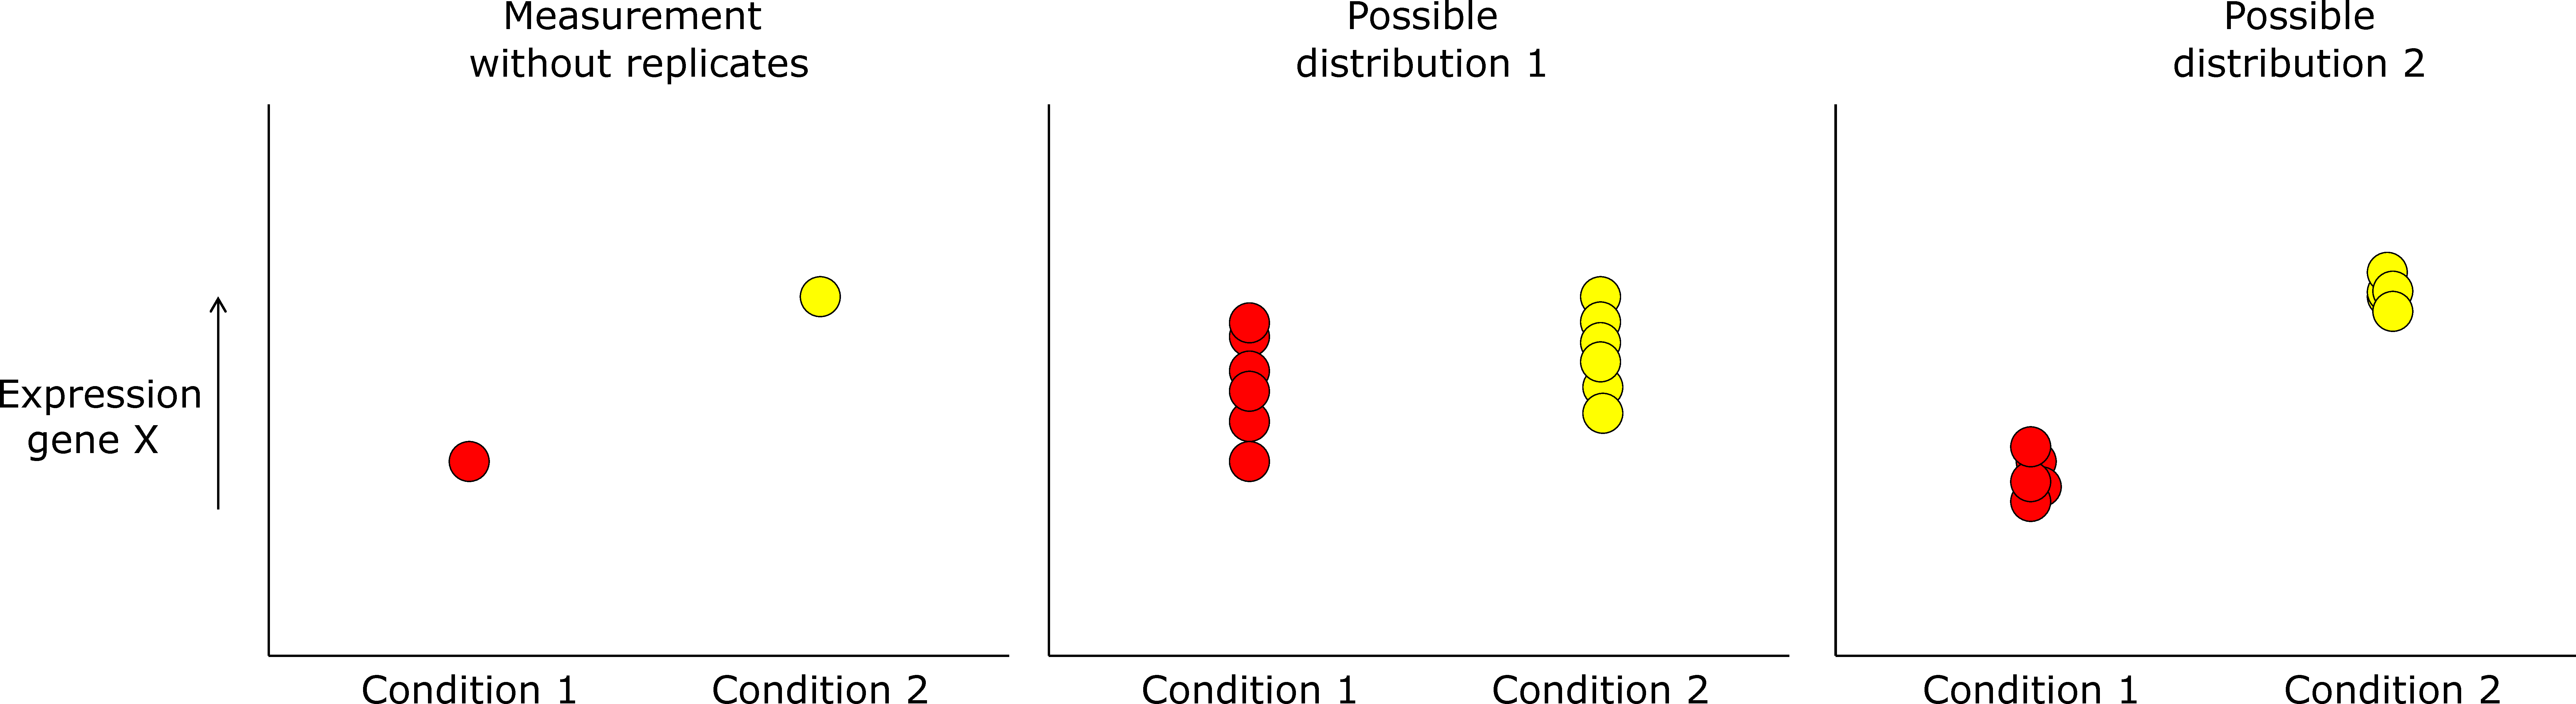
\includegraphics[width=0.7\linewidth]{files/compare-conditions-8407ef978ebe82f1ec8daa7e0e345017.pdf}
\caption[]{Difference in expression of gene X between two conditions measured without replicates and two possible distributions the measurement could have come from.
Credits: \href{https://creativecommons.org/licenses/by-nc/4.0/}{CC BY-NC 4.0} \cite{own_5_2024}.}
\label{compare_conditions}
\end{figure}

\begin{figure}[!htbp]
\centering
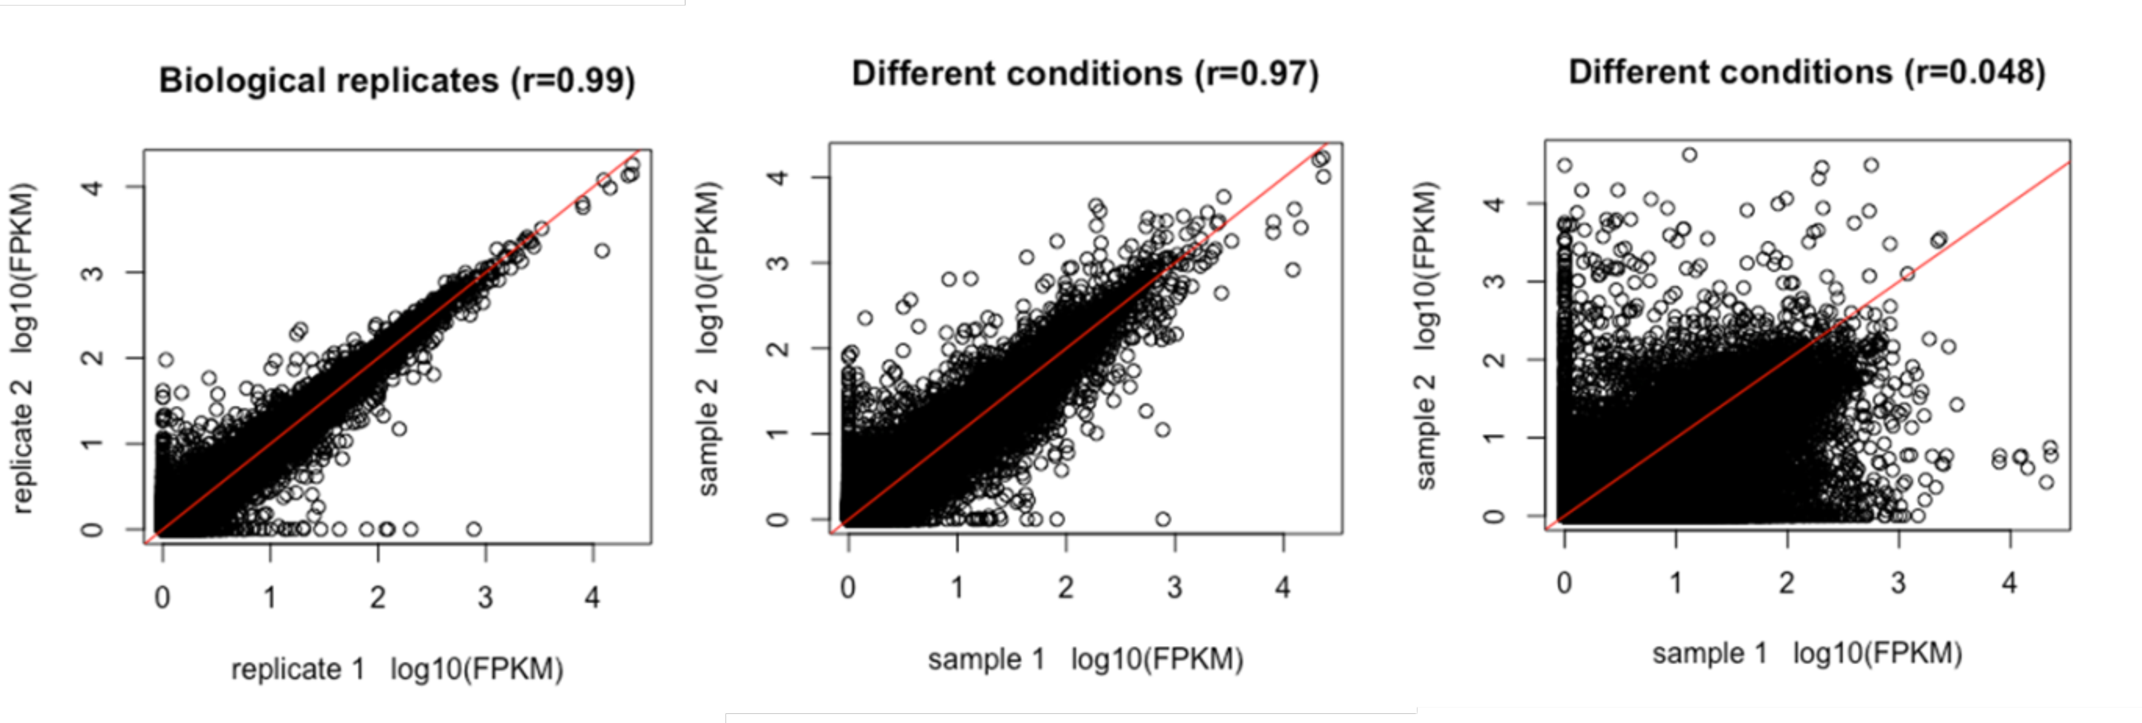
\includegraphics[width=0.7\linewidth]{files/error-vs-conditions-a7676036fef9e2c0267703c8b99477a5.pdf}
\caption[]{Comparison of FPKM values between 2 replicates (left) and two conditions (middle and right).
The correlation between replicates should be very high, the differences between two conditions can be small (middle) or large (right).
Credits: \href{https://creativecommons.org/licenses/by-nc/4.0/}{CC BY-NC 4.0} \cite{own_5_2024}.}
\label{error_vs_conditions}
\end{figure}

% #% Figure error_vs_conditions is saved as an svg but is not actually a vectorized image. Harm does not have the R file anymore.


\bigskip
\centerline{\rule{13cm}{0.4pt}}
\bigskip

\subparagraph{Visualization}

\begin{figure}[!htbp]
\centering
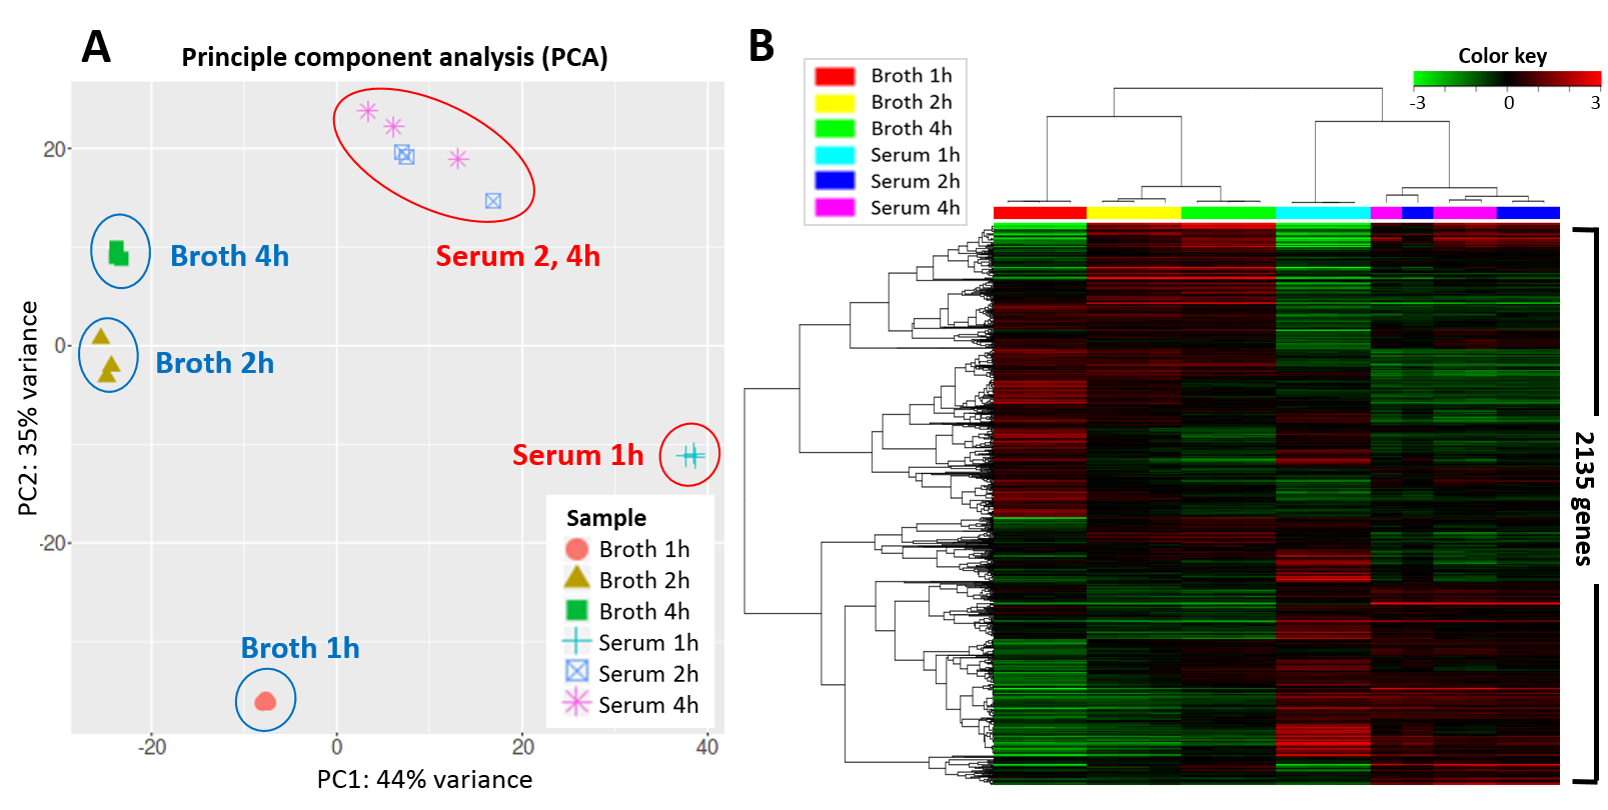
\includegraphics[width=0.7\linewidth]{files/streptococcus-pca-he-c98913885b96facdbea63add0f2be9fb.png}
\caption[]{Visualization of the expression of 2,135 genes in \textit{Streptococcus parauberis}
after 1, 2, and 4 hours of growth in two different media: fish serum and
broth. Each condition has been measured on 3 replicates. Left: a Principal
Component Analysis (PCA) that shows there is a major separation (44\% of the variance)
between the two media and that there is clear progression along time.
Note that there is not much expression difference after 2 and 4 hours of
growth on serum. Right: a heatmap visualizes the entire dataset, with colours
indicating z-score normalized expression values: green is low, black is
medium and red is high expression. Rows are genes, columns indicate growth
condition, both are clustered.
Credits: \href{https://creativecommons.org/licenses/by/4.0/}{CC BY 4.0} \cite{streptococcus_pca_heatmap_2021}.}
\label{streptococcus_pca_heatmap}
\end{figure}

While omics data can be analysed in for example Microsoft Excel, it is very
hard to make sense of a data matrix with tens of thousands of genes and
dozens to hundreds of samples. It is therefore wise to first use methods to
visualize or summarize the data to see whether major patterns or outliers
can already be detected. A widely used visualization is the so-called
heatmap, an image of the matrix (genes-by-samples) where each measurement is represented by a
colour. If the data is clustered along both genes and samples,
interesting patterns may be easy to spot. A second approach often used in
initial data exploration is Principal Component Analysis (PCA), which plots
samples (or genes) along the main axes of variation in the data. If colour or
markers are added, a PCA plot serves very well to detect groups and outliers.
Both visualizations are illustrated in Figure~\ref{streptococcus_pca_heatmap}.


\bigskip
\centerline{\rule{13cm}{0.4pt}}
\bigskip

\subparagraph{Differential abundance}

\begin{figure}[!htbp]
\centering
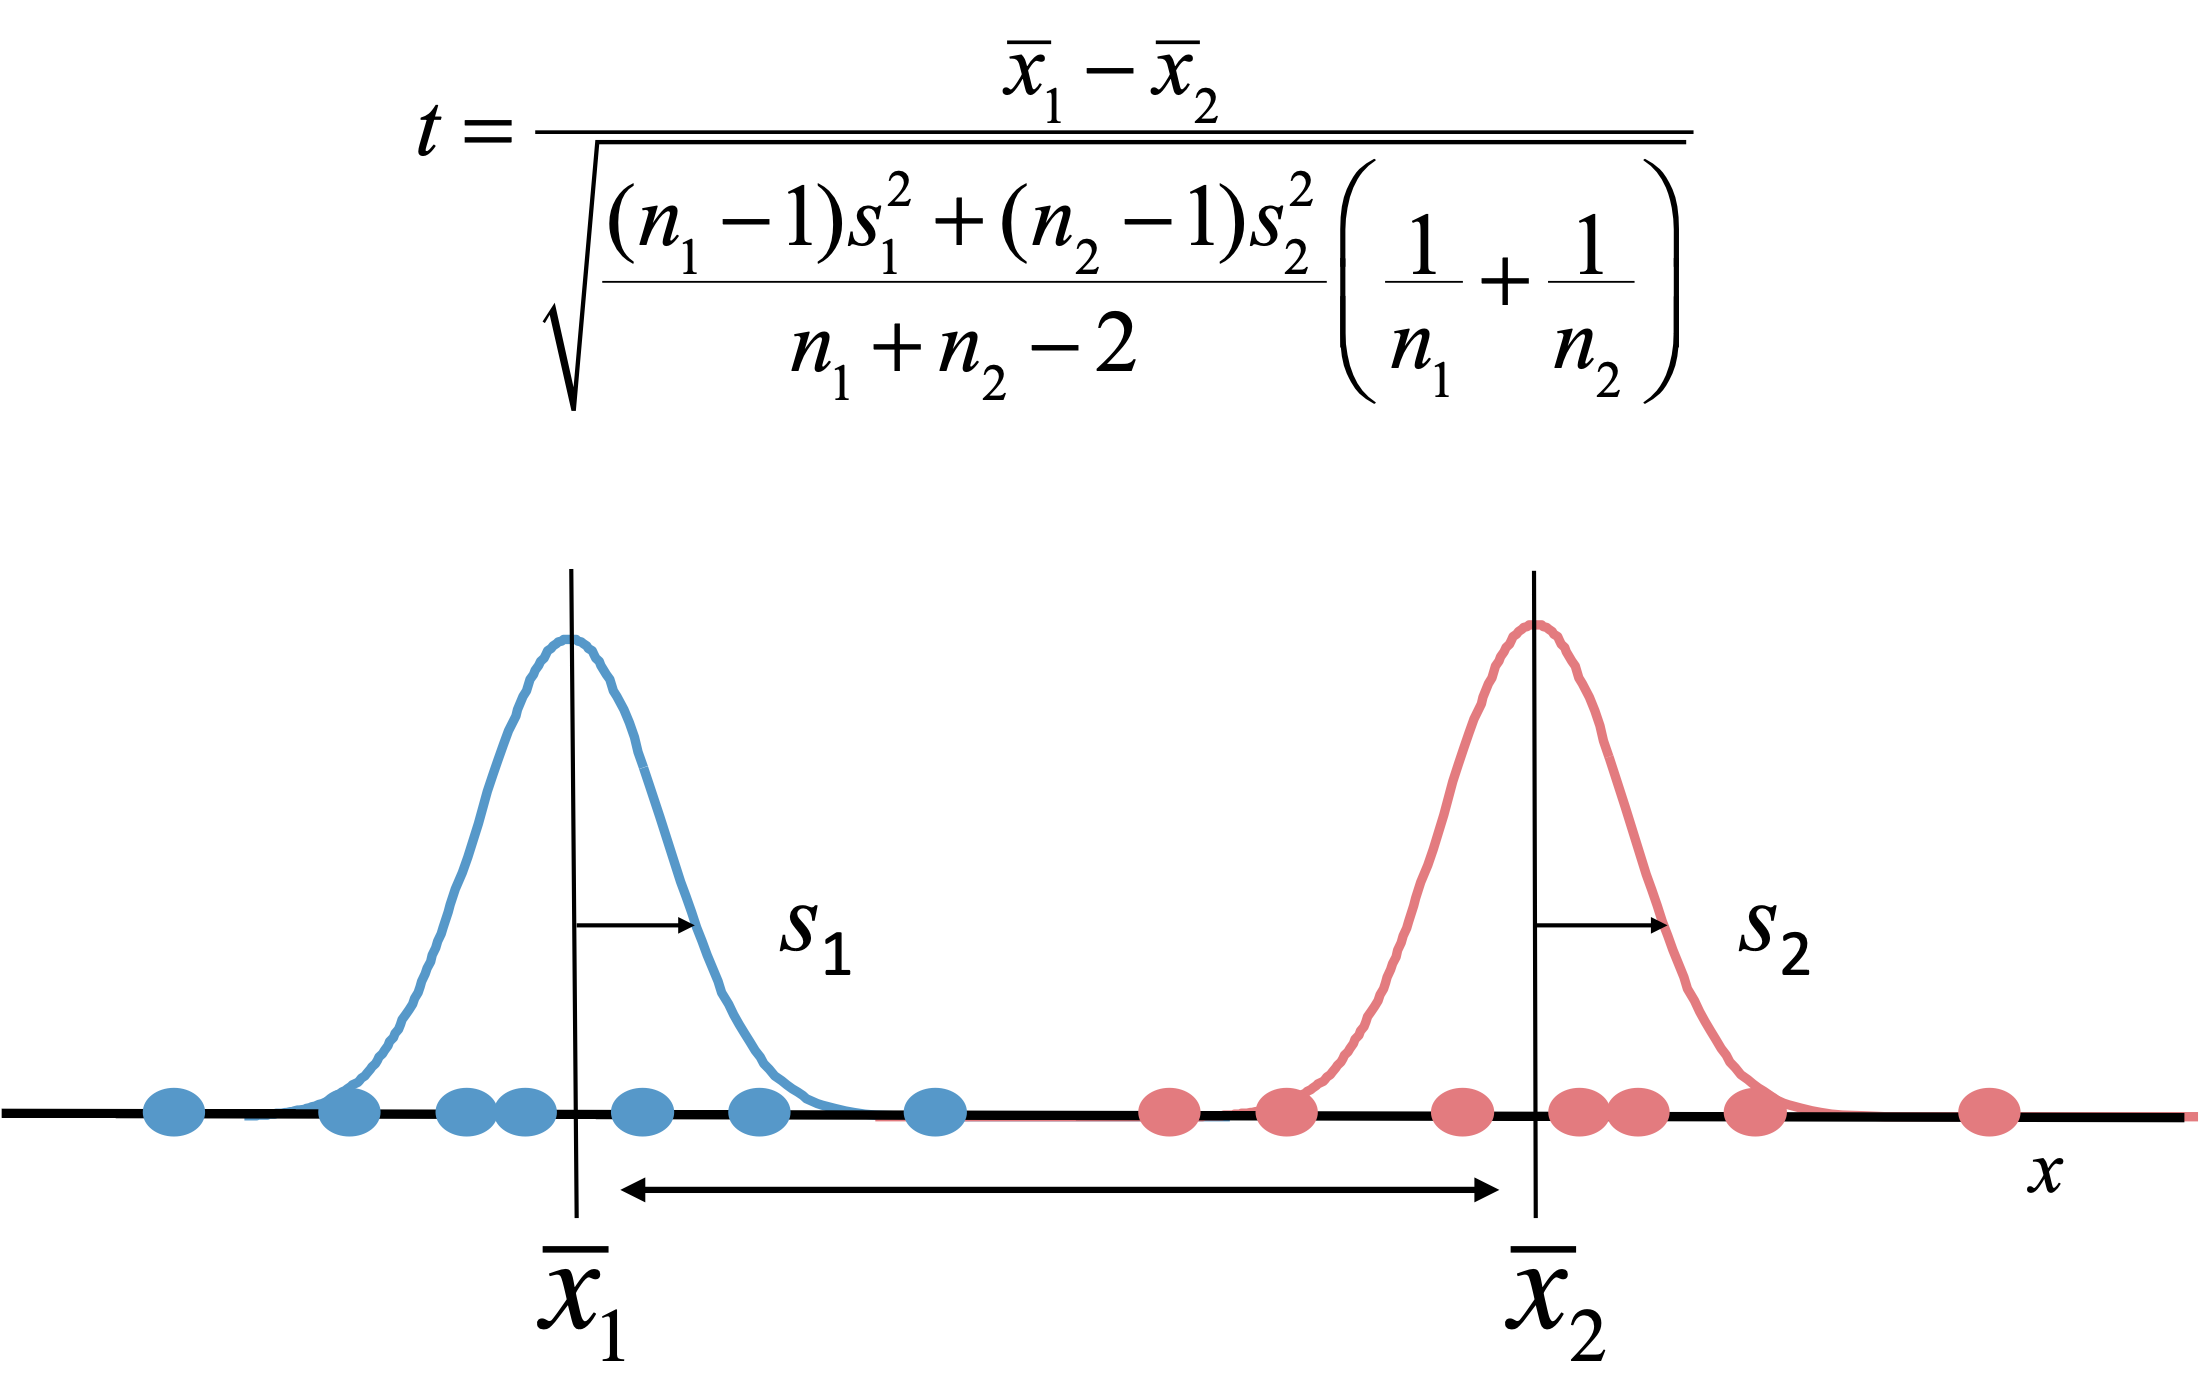
\includegraphics[width=0.7\linewidth]{files/t-test-bee788aad21f28abe4dd4b15ed86671b.png}
\caption[]{The simplest test for differential abundance of a gene between two
conditions is the \textit{t}-test. The \textit{t}-statistic is a measure for the
difference between the means \textit{x} of two distributions, corrected by the
uncertainty expressed in terms of their standard deviation \textit{s}. A \textit{p}-value,
the probability that we find a \textit{t}-statistic as large or larger by chance,
can be calculated using the \textit{t}-distribution.
Credits: \href{https://creativecommons.org/licenses/by-nc/4.0/}{CC BY-NC 4.0} \cite{own_5_2024}.}
\label{t_test}
\end{figure}

Perhaps the most widely used analysis on omics data, the goal here is to
compare abundance levels between two classes, conditions, strains, cell
types, etc. - for example, healthy vs. diseased tissue, with or without a
certain drug, in different growth conditions, etc. The simplest approach is
to collect a number of replicate measurements under both conditions and, for
each gene perform a simple statistical test such as the \textit{t}-test
(Figure~\ref{t_test}). Each test
gives a \textit{p}-value, and genes with a \textit{p}-value below a certain
threshold, say 5\%, could then called significantly differentially expressed.
There are two caveats:

\begin{enumerate}
\item If you perform an individual test for each of thousands of genes, at a
threshold of 5\% you would still incorrectly call many hundreds to thousands
genes differentially expressed. To solve this, \textit{p}-values are generally
\textit{adjusted} for multiple testing, i.e., made larger.
\item If the variation (standard deviation \textit{s} in Figure~\ref{t_test}) is low enough, a
small difference can become significant even if the actual abundance
difference is small. Therefore, in many experiments an additional
requirement to select genes is that the fold change is large enough. Often,
this is expressed as log2(fold change), where +1 means that a gene is 2x
more expressed, +2 means 4x more expressed, -1 means 2x less expressed and
so on.
\end{enumerate}

There are a number of similar, but more sophisticated approaches that better
match with experimental follow-up, but these are out of scope for this
book.


\bigskip
\centerline{\rule{13cm}{0.4pt}}
\bigskip

\subparagraph{Time series analysis}

\begin{figure}[!htbp]
\centering
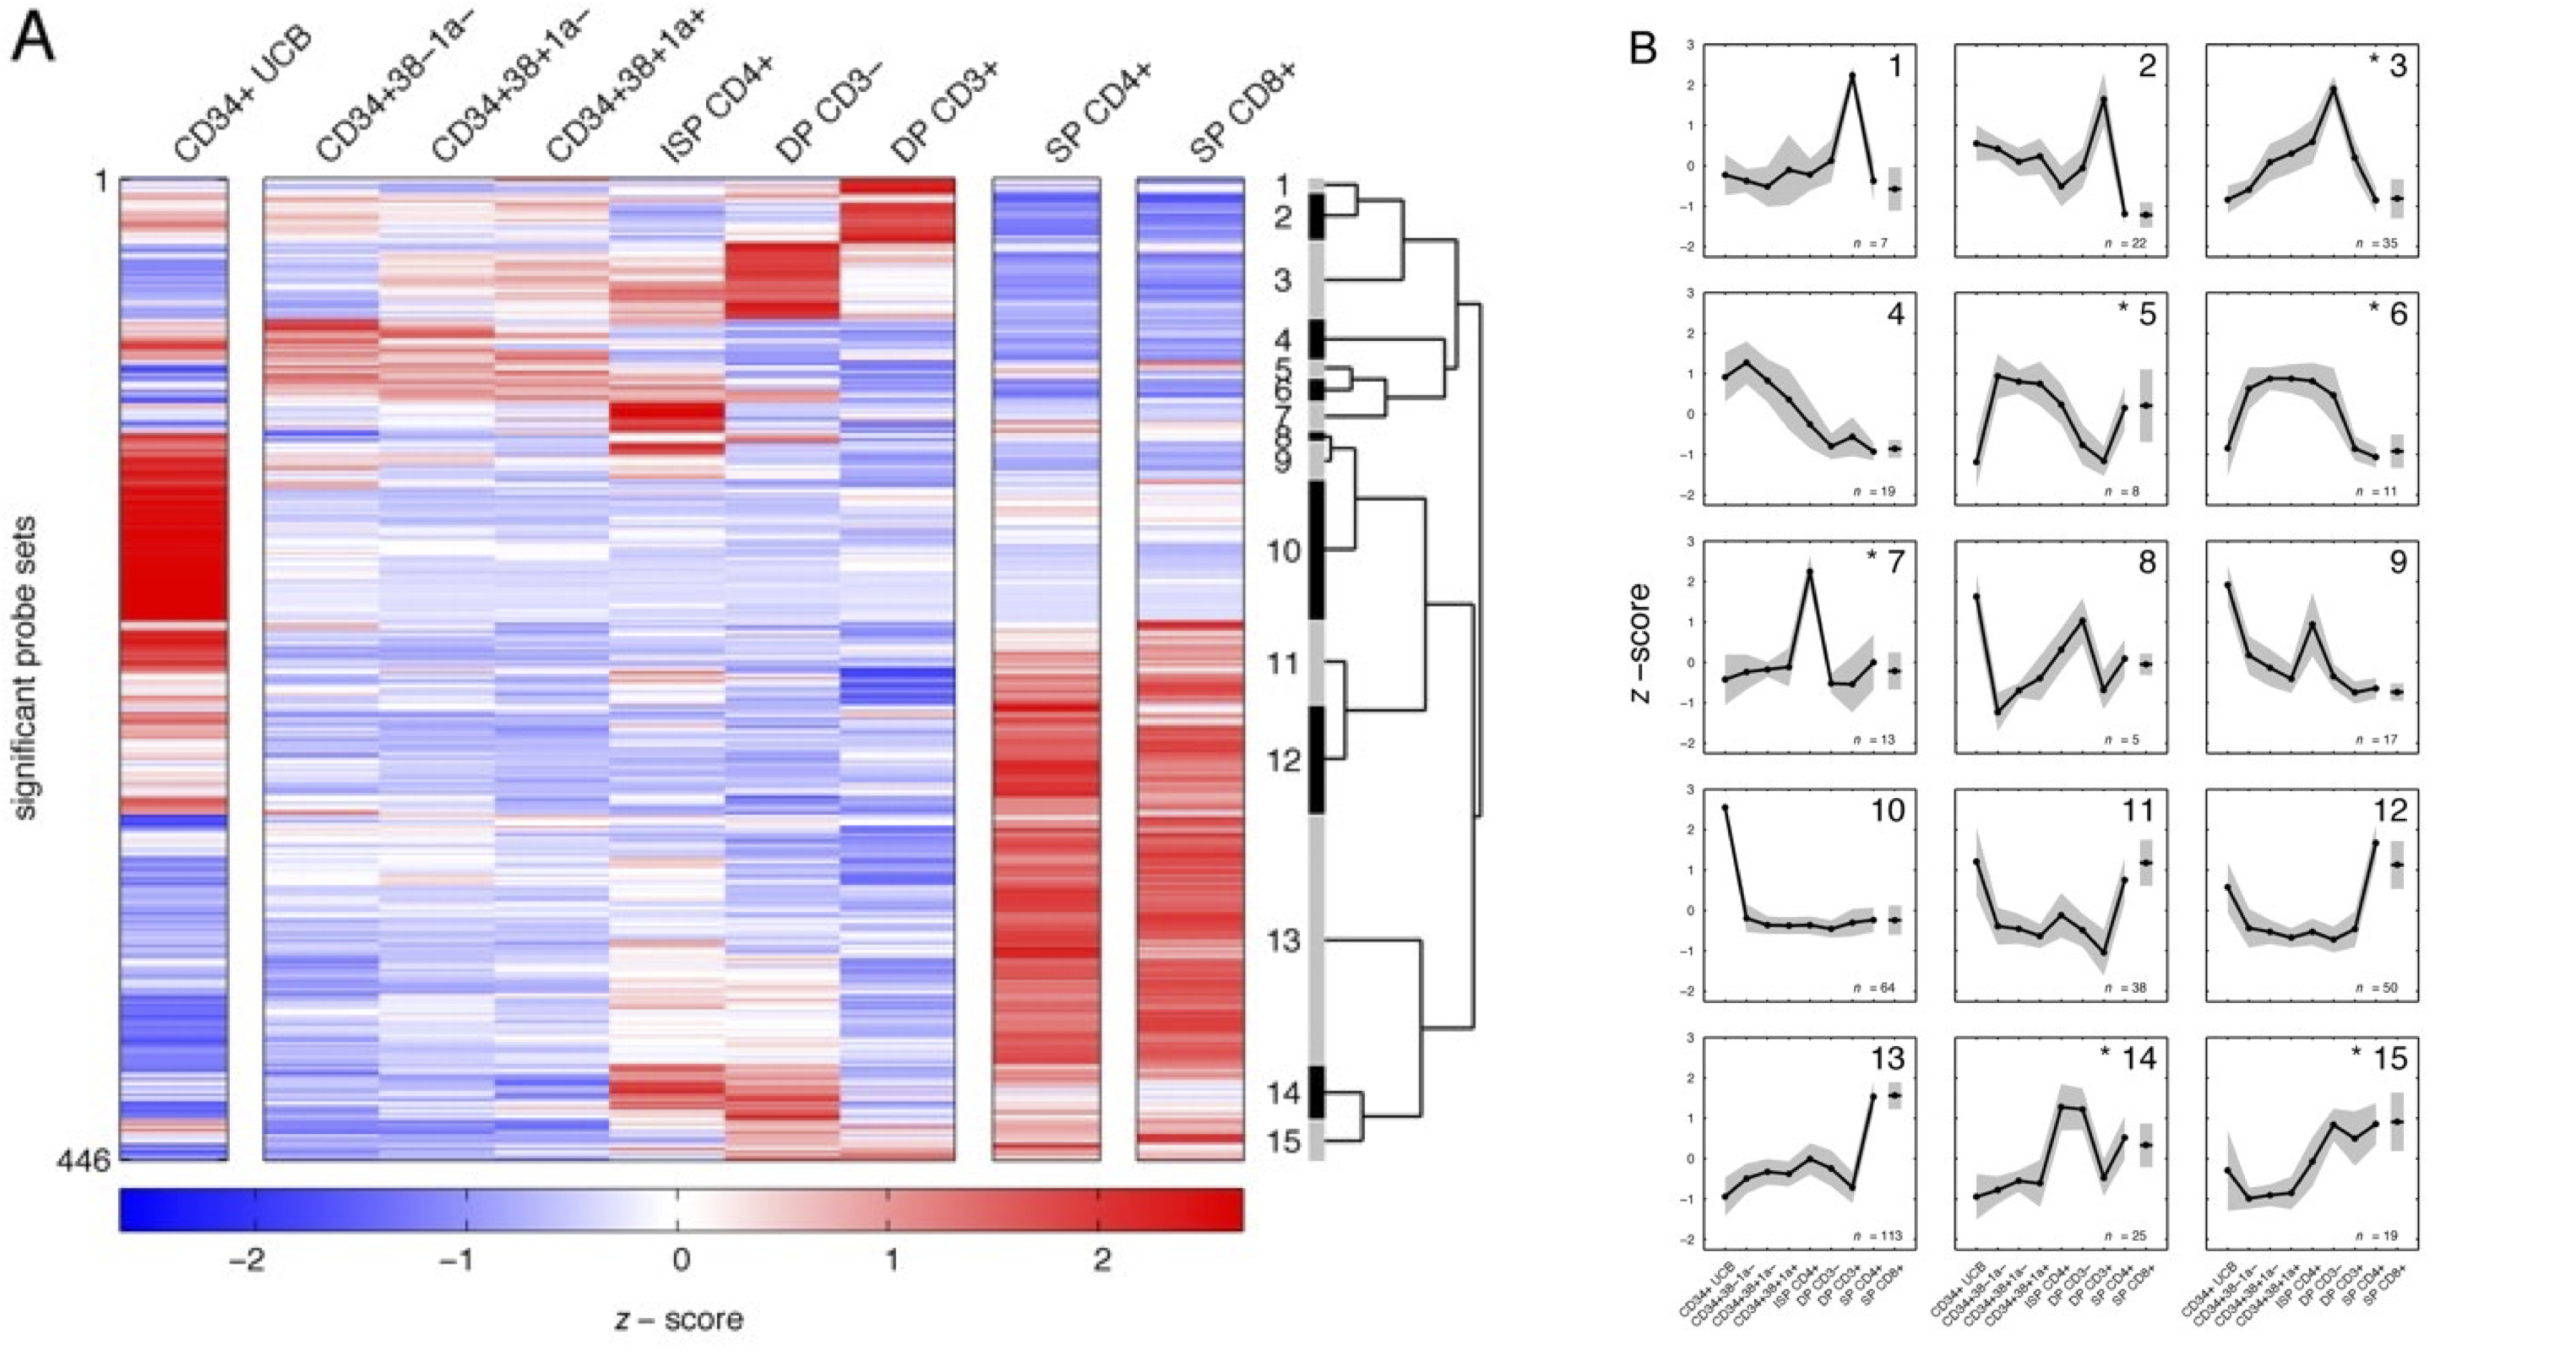
\includegraphics[width=0.7\linewidth]{files/time-series-d0b6bf77170bca1086f7738a98d742ee.png}
\caption[]{Transcriptomics of various stages of T-cell development, i.e., a time
series analysis. Left: heatmap of the 446 genes with most variable gene
expression levels, clustered into 15 clusters. Right: average expression
profiles of each cluster show that different groups of genes peak in
expression in different development stages. These genes may be regulated in
the same way and be active in similar biological processes.
Credits: \href{https://creativecommons.org/licenses/by-nc-sa/4.0/}{CC BY-NC-SA 4.0} \cite{time_series_2005}.}
\label{time_series}
\end{figure}

Often it is more interesting to follow abundance over time rather than
compare it at one specific timepoint, e.g., when tracking the response to a
drug, a change in growth conditions, regulation of organ development, and so
on. Given the cost of omics measurements, a major challenge is to select
optimal time points for sampling, balancing the information obtained with
the investment. Subsequent analyses include clustering to find similarly
regulated genes (see [below \#chapter5\_clustering)) and more advanced methods that try to identify
regulatory interactions by seeing which gene increase/decrease precedes that
of another (set of) gene(s). Figure~\ref{time_series} provides an example.


\bigskip
\centerline{\rule{13cm}{0.4pt}}
\bigskip

\subparagraph{Classification}

Classification is related to differential abundance analysis, in that it
tries to find genes that best explain the difference between conditions.
However, here the goal is actually to predict the condition of a new (additional)
sample based on a limited set of gene expression levels, as accurately as possible.
Applications are mainly found in medicine, such as diagnosis and prognosis,
but are also used to distinguish different cell types, growth stages, etc.


\bigskip
\centerline{\rule{13cm}{0.4pt}}
\bigskip

\subparagraph{Clustering}\label{chapter5_clustering}

Clustering methods attempt to find groups of genes that have similar
abundance profiles over all samples, or (vice versa) samples that have
similar abundance profiles over all genes. We call such genes or samples
co-expressed. Based on the guilt-by-association principle, correlation
can be used to learn about the function of genes - ``if the expression of gene
A is similar to that of gene B with a certain function F, then gene A likely
also has function F''. This can help identify genes involved in similar
processes or pathways: co-expressed genes can be co-regulated, code for
interacting proteins, etc. For samples, it can help identify for example
disease subtypes, different genotypes, etc. that may be helpful to learn
about different outcomes. Clustering is often used to order the rows and
columns of a heatmap (as in Figure~\ref{streptococcus_pca_heatmap} and Figure~\ref{time_series}), after
which obvious clusters should become visible as large colour blocks.


\bigskip
\centerline{\rule{13cm}{0.4pt}}
\bigskip

\subparagraph{Enrichment}

\begin{figure}[!htbp]
\centering
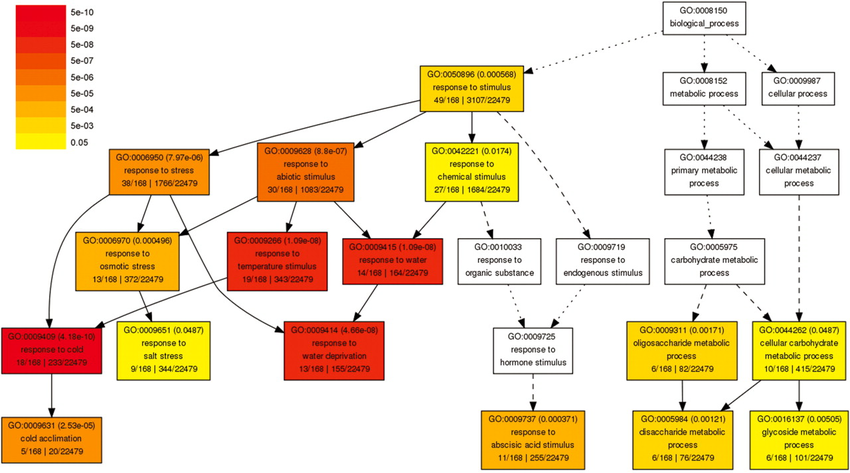
\includegraphics[width=0.7\linewidth]{files/GO-enrichment-bfc30ac36543d5ffd837c9831ca15ddd.png}
\caption[]{An example part of the Gene Ontology (GO), in the biological process category.
Lower-level terms are specific instantiations of the higher-level ones. In
this figure, GO terms are coloured according to the \textit{p}-value in an
enrichment test.
Credits: \href{https://creativecommons.org/licenses/by-nc/4.0/}{CC BY-NC 4.0} \cite{own_5_2024}.}
\label{go_enrichment}
\end{figure}

A final often used analysis is enrichment, in which we use gene functional
annotation to learn about a set of genes, such as a list of differentially
expressed genes or a cluster. The most widely used annotation for genes is
the Gene Ontology, a structured dictionary of terms that describe the
molecular functions of genes and their involvement in biological processes
or cellular components at different levels of detail (Figure~\ref{go_enrichment}). A statistical test
then assesses how significantly often (more than by chance) we find a
certain annotation in our list of genes. Like differential abundance, the
\textit{p}-values produced should be adjusted for multiple testing. The resulting
significant annotations can help interpret the outcome of an experiment at a
higher level than that of individual genes.


\bigskip
\centerline{\rule{13cm}{0.4pt}}
\bigskip

\paragraph{Outlook}

This section on omics data analysis is likely the most prone
to obsolescence. We have only touched upon or even left out recent
developments in single-molecule measurements of DNA, RNA, and proteins, of
single-cell and spatial omics analysis, where molecules are measured in
individual cells or at grid points in tissues, and accompanying developments
in deep learning that promise to provide foundation models to capitalize on
the large volumes of omics data in order to learn the ``language'' of DNA and
proteins and to solve specific tasks. The end
goal, \href{https://www.wholecellviz.org/viz.php\#replication}{a systems biology simulation of the living
cell}, is still far from
reality, but may be reached sooner than we now believe possible.


\bigskip
\centerline{\rule{13cm}{0.4pt}}
\bigskip

\subsubsection{Practical assignments}

This practical contains questions and exercises to help you process the study materials of Chapter 5.
You have 2 mornings to work your way through the exercises.
In a single session you should aim to get about halfway through this guide (i.e., day 1: assignment 1-3, day 2: assignment 4, 5 and project preparation exercise).
Use the time indication to make sure that you do not get stuck in one assignment.
These practical exercises offer you the best preparation for the project.
Especially the \textbf{project preparation exercise} at the end is a good reflection of the level that is required to write a good project report.
Make sure that you develop your practical skills now, in order to apply them during the project.

\textbf{Note, the answers will be published after the practical!}

\begin{framed}
\textbf{Clustering, 30 minutes}\\
If all went well, you found a correlation between the expression of BCL11B and RHOH in some tissues.
It is easier to find such relations by performing clustering, i.e., finding groups of genes and/or groups of samples that have similar expression.
Such clusters can help you learn about functional relations between genes that cluster together, or phenotypic relations between samples that cluster together.
For the CCLE, a nice interactive viewer is available \href{https://maayanlab.github.io/CCLE\_Clustergrammer/}{here}.
Open the page and select the ``Bone'' subset.

\begin{enumerate}
\item In the main figure, the so-called \textbf{heatmap}, what do blue and red pixels correspond to? Note that you can zoom in and scroll around using the mouse; and do read the text below the figure.
\item What is the expression level of BCL11B (use the search box if needed) in sample RDES?
\item On the right and at the bottom, the clusters are indicated by grey bars. How many groups of genes do you see initially? And how many groups of samples? Do you think that is reasonable, given the gene expression values?
\item You can create fewer or more clusters using the ``volume slider buttons'' next to the clusters. Try these. Does it look OK to group the genes into more clusters? And the samples?
\item Zoom in on the gene names on the left. Is BCL11B indeed clustered with RHOH?
\item At the top, additional information on the samples is plotted (tissue, histology, etc.). Does one of the sample clusters correspond to a certain annotation?
\item The top left shows a number of Gene Ontology terms (recall from chapter~1 that occur more often in the set of genes involved in bone tumours than you would expect by chance (i.e., than if a set of genes of similar size were randomly drawn from all genes). We call this a \textbf{GO enrichment analysis}. The heights of the bars correspond to the p-values of this analysis; the higher the bar, the more significant the enrichment. Do the terms make sense?
\end{enumerate}
\end{framed}

\begin{framed}
\textbf{Differential gene expression, 45 minutes}\\
NCBI hosts the Gene Expression Omnibus, a database containing gene expression experiments - both microarrays and RNAseq. You can download and combine these data in various formats and analyse them on your own computer to potentially answer biological questions without performing measurements yourself. This course is too short to teach all the skills you need for reanalysing public data, but we can make use of an online tool called GEO2R to do some simple analyses in a web browser.

After completing this assignment, you should be able to interpret the results of differential expression analyses on quantitative data.

\begin{enumerate}
\item Visit the \href{https://www.ncbi.nlm.nih.gov/geo}{Gene Expression Omnibus}, search for sample series GSE69485 (microarray data) and read the summary and design of the study that produced this series. At the bottom you can find a list of samples. How many are there?
\item What type of microarray is used? You can get more information by searching GEO for GPL90. How many probesets are there (corresponding to the number of rows in the data table)? For how many genes?
\end{enumerate}

You can perform simple analyses on this data in GEO2R.
In this case, we will try to find genes differentially expressed between yeast grown in aerobic and anaerobic conditions, i.e., with oxygen vs. without oxygen.
To get started, return to the page for sample series GSE69485 and press the ``Analyze with GEO2R'' button at the bottom of the page.
You will see a list of all samples, which you can now assign to different groups.
First, click ``Define groups'' (at the top) to create two groups, say ``aerobic'' and ``anaerobic''.
Then select all four samples taken during exponential growth phase (also late/end) under anaerobic conditions and assign them to the anaerobic group, by clicking ``anaerobic'' in the group list.
Do the same for the four aerobic exponential growth phase samples.

\begin{enumerate}[resume]
\item Scroll down and press the ``Analyze'' button. After some processing, a number of graphs are shown that present expression levels, fold changes, differentially expressed genes (blue/red) etc. The ``expression density'' plot contains the overall distributions of the expression values of all genes per sample; if these distributions look very different, for example due to differences in the measurement setup, this may point to problems. Do these arrays look like they can be compared?
\end{enumerate}

Below the figures you should see a list of Affymetrix probe sets (under ``ID''), sorted by (adjusted) \textit{p}-values.
The logFC column indicates the log\textsubscript{2} fold change: 0 for no change, positive for genes more highly expressed under anaerobic conditions and negative for genes more highly expressed under aerobic conditions (or vice versa, depending on which group you created first).

\begin{enumerate}[resume]
\item What is the most significantly differentially expressed gene here (the one with the lowest \textit{p}-value)?
\item You can inspect the underlying expression values by clicking on the corresponding row in the table, this will show a plot with the expression in each sample; the ``Sample values'' button will show the actual measurements. Compare the expression ranges for the top three genes. What do you notice?
\item To learn more about the differentially expressed genes, you can add Gene Ontology (GO) information. To do so, click ``Select columns'' above the table and select ``GO: Function'', ``GO: Process'' and ``GO: Component''. Then press ``Set''. What types of functions do you notice in the top 20 genes?
\end{enumerate}


\bigskip
\centerline{\rule{13cm}{0.4pt}}
\bigskip

\textbf{Optional (20 minutes)}

Ideally, the results obtained are corroborated by additional experiments.
In GEO, another study is available that focused on the effect of engineering amylase genes in yeast, producing series GSE38848.

\begin{enumerate}[resume]
\item Use GEO2R on series GSE38848 to find genes differentially expressed under anaerobic and aerobic conditions in the reference strain (NC) only. Do you find the same genes? The same functions?
\end{enumerate}


\bigskip
\centerline{\rule{13cm}{0.4pt}}
\bigskip

Note that this was just a quick tour of a number of tools to interpret omics data, for some very specific datasets (transcriptomics in human cancer cells and yeast
cells). However, the underlying analyses -- differential expression, clustering,
principal component analysis etc. -- can be widely applied on most quantitative --
omics datasets. If you want to dive deeper, you will need to use more advanced
(statistical) methods which are taught in other courses.
\end{framed}

\begin{framed}
\textbf{\textbf{Project Preparation Exercise}}\\
An assignment focusing on how to write a good project report is available on BrightSpace.
The results will be discussed at the end of the Week 5 recap lecture


\bigskip
\centerline{\rule{13cm}{0.4pt}}
\bigskip

Explore tissue-specific gene expression of ARF5 and IAA5.
For this, you can use some other (plant-specific) resources than the human-centered ones you used above, e.g., \href{https://www.ebi.ac.uk/gxa/}{Expression Atlas} (also accessible through UniProt, under ``Expression'') or \href{https://bar.utoronto.ca/}{BAR}, the Bio-Analytic Resource for Plant Biology.

Describe the following items in a few bullet points each.
You may include up to two figures or tables.

\begin{enumerate}
\item \textbf{Materials \& Methods} What did you do? Which data, databases and tools did you use, and why did you choose these? What important settings did you select?
\item \textbf{Results} What did you find, what are the main results? Report the relevant data, numbers, tables/figures, and clearly describe your observations.
\item \textbf{Discussion \& Conclusion} Do the results make sense? Are they according to your expectation or do you see something surprising? What do the results mean, how can you interpret them? Do different tools agree or not? What can you conclude? Make sure to describe the expectations and assumptions underlying your interpretation.
\end{enumerate}
\end{framed}

\subsubsection{Glossary}

\subsubsection{References}